%implementing document formatting:
\documentclass[a4paper,11pt,fleqn,dvipsnames,oneside,openright,oldfontcommands]{memoir} 	% Openright aabner kapitler paa hoejresider (openany begge)


%%%%%%%%% Indsat random
%makes it possible to refer to the name of a chapter rather than just the number.
\usepackage{nameref}
\usepackage{pdfpages}
\usepackage{marvosym}
\usepackage{setspace}
\usepackage{graphicx} % For at sætte 2 billeder ved siden af hinanden

%package for writing program code in latex
\usepackage{listings}
%%%%%%%%%%%%%%%%%%%%%%

% ¤¤ Oversaettelse og tegnsaetning ¤¤ %
\usepackage[T1]{fontenc}					% Output-indkodning af tegnsaet (T1)
\usepackage[danish]{babel}					% Dokumentets sprog
\usepackage[utf8]{inputenc}					% Input-indkodning af tegnsaet (UTF8)
\usepackage{ragged2e,anyfontsize}			% Justering af elementer
\usepackage{fixltx2e}						% Retter forskellige fejl i LaTeX-kernen							
				
																							
% ¤¤ Figurer og tabeller (floats) ¤¤ %
\usepackage{graphicx} 						% Haandtering af eksterne billeder (JPG, PNG, EPS, PDF)
%\usepackage{eso-pic}						% Tilfoej billedekommandoer paa hver side
%\usepackage{wrapfig}						% Indsaettelse af figurer omsvoebt af tekst. \begin{wrapfigure}{Placering}{Stoerrelse}
\usepackage{multirow}                		% Fletning af raekker og kolonner (\multicolumn og \multirow)
\usepackage{multicol}         	        	% Muliggoer output i spalter
\usepackage{rotating}						% Rotation af tekst med \begin{sideways}...\end{sideways}
\usepackage{colortbl} 						% Farver i tabeller (fx \columncolor og \rowcolor)
\usepackage{xcolor}							% Definer farver med \definecolor. Se mere: http://en.wikibooks.org/wiki/LaTeX/Colors
\usepackage{flafter}						% Soerger for at floats ikke optraeder i teksten foer deres reference
\let\newfloat\relax 						% Justering mellem float-pakken og memoir
\usepackage{float}							% Muliggoer eksakt placering af floats, f.eks. \begin{figure}[H]
\usepackage{array,booktabs,xcolor,longtable} % kan lave \hdashline i tabellertabe
\usepackage{arydshln}
\usepackage{tabu}

	
	
% ¤¤ Matematik mm. ¤¤
\usepackage{amsmath , amsthm , amsfonts , amssymb, float, stmaryrd} 		% Avancerede matematik-udvidelser
%\usepackage{mathtools}						% Andre matematik- og tegnudvidelser
\usepackage{textcomp}                 		% Symbol-udvidelser (f.eks. promille-tegn med \textperthousand )
\usepackage{rsphrase}						% Kemi-pakke til RS-saetninger, f.eks. \rsphrase{R1}
\usepackage[version=3]{mhchem} 				% Kemi-pakke til flot og let notation af formler, f.eks. \ce{Fe2O3}
\usepackage{siunitx}						% Flot og konsistent praesentation af tal og enheder med \si{enhed} og \SI{tal}{enhed}
\sisetup{output-decimal-marker = {,}}		% Opsaetning af \SI (DE for komma som decimalseparator) 

% ¤¤ Referencer og kilder ¤¤ %
\usepackage[danish]{varioref}				% Muliggoer bl.a. krydshenvisninger med sidetal (\vref)
\usepackage[numbers]{natbib}				% Udvidelse med naturvidenskabelige citationsmodeller
%\usepackage{xr}							% Referencer til eksternt dokument med \externaldocument{<NAVN>}
%\usepackage{glossaries}					% Terminologi- eller symbolliste (se mere i Daleifs Latex-bog)
\usepackage{lastpage}					% Gør det mulig at refere til sidste side 

% ¤¤ Misc. ¤¤ %
\usepackage{listings}						% Placer kildekode i dokumentet med \begin{lstlisting}...\end{lstlisting}
\usepackage{lipsum}							% Dummy text \lipsum[..]
\usepackage[shortlabels]{enumitem}			% Muliggoer enkelt konfiguration af lister
\usepackage{pdfpages}						% Goer det muligt at inkludere pdf-dokumenter med kommandoen \includepdf[pages={x-y}]{fil.pdf}	
\pdfoptionpdfminorversion=6					% Muliggoer inkludering af pdf dokumenter, af version 1.6 og hoejere
\pretolerance=2500 							% Justering af afstand mellem ord (hoejt tal, mindre orddeling og mere luft mellem ord)


% Kommentarer og rettelser med \fxnote. Med 'final' i stedet for 'draft' udloeser hver note en error i den faerdige rapport.
\usepackage[footnote,draft,danish,silent,nomargin]{fixme}		


%%%% CUSTOM SETTINGS %%%%

% ¤¤ Marginer ¤¤ %
\setlrmarginsandblock{3.0cm}{2.5cm}{*}		% \setlrmarginsandblock{Indbinding}{Kant}{Ratio}
\setulmarginsandblock{2.5cm}{3.0cm}{*}		% \setulmarginsandblock{Top}{Bund}{Ratio}
\checkandfixthelayout 						% Oversaetter vaerdier til brug for andre pakker

%	¤¤ Afsnitsformatering ¤¤ %
\setlength{\parindent}{6mm}           		% Stoerrelse af indryk
\setlength{\parskip}{0mm}          			% Afstand mellem afsnit ved brug af double Enter
\linespread{1,1}							% Linie afstand



% ¤¤ Indholdsfortegnelse ¤¤ %
\setsecnumdepth{subsection}		 			% Dybden af nummerede overkrifter (part/chapter/section/subsection)
\maxsecnumdepth{subsection}					% Dokumentklassens graense for nummereringsdybde
\settocdepth{section} 					% Dybden af indholdsfortegnelsen

% ¤¤ Lister ¤¤ %
\setlist{
  topsep=0pt,								% Vertikal afstand mellem tekst og listen
  itemsep=-1ex,								% Vertikal afstand mellem items
} 

%hyperlinks in the tabel of contents - comment this out before the report is printed.
\usepackage{hyperref}
\hypersetup{
	bookmarks = true,  % Show 'bookmark'-frame in pdf.
	colorlinks = true, % True = colored links, False = framed links.
	citecolor = black,  % Link color for references.
	linkcolor = black,  % Link color in table of contents.
	urlcolor = black,   % Link color for extern URLs.
}

% ¤¤ Opsaetning af figur- og tabeltekst ¤¤ %
\usepackage{caption}
%\usepackage{subcaption}
\captionnamefont{\small\bfseries\itshape}	% Opsaetning af tekstdelen ('Figur' eller 'Tabel')
\captiontitlefont{\small}					% Opsaetning af nummerering
\captiondelim{. }							% Seperator mellem nummerering og figurtekst
\hangcaption								% Venstrejusterer flere-liniers figurtekst under hinanden
%\captionwidth{0.9\textwidth}					% Bredden af figurteksten
\setlength{\belowcaptionskip}{0pt}			% Afstand under figurteksten
\captionsetup[figure]{labelfont={bf,it},font={it}} % sætter nummer til fed og kursis. Resten til fed + skriften er mindre end resten
\captionsetup[table]{labelfont={bf,it},font={it}} 


% ¤¤ Opsaetning af listings ¤¤ %

\definecolor{commentGreen}{RGB}{34,139,24}
\definecolor{stringPurple}{RGB}{208,76,239}

\lstset{language=Matlab,					% Sprog
	basicstyle=\ttfamily\scriptsize,		% Opsaetning af teksten
	keywords={for,if,while,else,elseif,		% Noegleord at fremhaeve
			  end,break,return,case,
			  switch,function},
	keywordstyle=\color{blue},				% Opsaetning af noegleord
	commentstyle=\color{commentGreen},		% Opsaetning af kommentarer
	stringstyle=\color{stringPurple},		% Opsaetning af strenge
	showstringspaces=false,					% Mellemrum i strenge enten vist eller blanke
	numbers=left, numberstyle=\tiny,		% Linjenumre
	extendedchars=true, 					% Tillader specielle karakterer
	columns=flexible,						% Kolonnejustering
	breaklines, breakatwhitespace=true,		% Bryd lange linjer
}

% ¤¤ Navngivning ¤¤ %
\addto\captionsdanish{
	\renewcommand\appendixname{Bilag}
	\renewcommand\contentsname{Indholdsfortegnelse}	
	\renewcommand\appendixpagename{Bilag}
	\renewcommand\appendixtocname{Bilag}
	\renewcommand\cftchaptername{\chaptername~}				% Skriver "Kapitel" foran kapitlerne i indholdsfortegnelsen
	\renewcommand\cftappendixname{\appendixname~}			% Skriver "Appendiks" foran appendiks i indholdsfortegnelsen
}

% ¤¤ Kapiteludssende ¤¤ %
%\definecolor{numbercolor}{gray}{0.7}		% Definerer en farve til brug til kapiteludseende
%\newif\ifchapternonum

\makechapterstyle{AAU}
{
	% Afstand mellem sidehovedet og kapitel+tal+kapitelnavnet defineres til:
	\setlength{\beforechapskip}{0cm}

	% Afstanden mellem kapitelnavnet og body-teksten defineres til:
	\setlength{\afterchapskip}{2cm}

	% Typografiopsætningen til kapitel+tal defineres til:
	\renewcommand\chapnamefont{\sffamily\bfseries\LARGE\raggedright}
	
	% Typografiopsætningen til kapitel+tal defineres til:
	\renewcommand\chaptitlefont{\sffamily\bfseries\huge\color[cmyk]{1.00,0.38,0.00,0.64}}

	% Forårsager, at der til kapitlet også tilføjes dets respektive tal:
	\renewcommand\chapternamenum{}
	\renewcommand\printchapternum
	{
		\makebox[0pt][l]
		{
			\color[cmyk]{1.00,0.38,0.00,0.64}
			\hspace{0.1cm}
			\resizebox{!}{1cm}{\chapnamefont\bfseries\sffamily\thechapter}
		}
	}
	
	% Definitionen af linjenstykket mellem ``Kapitel #'' samt ``kapitelnavnet'':
			\renewcommand\afterchaptertitle{\par\hspace{1.5cm}\hrule height 1pt\vskip\midchapskip}
}

% Aktivering af selve kapitellayoutet med dét navn, som definerer kapitellayoutet (ses fra tidligere):
\chapterstyle{AAU}

%\makechapterstyle{jenor}{					% Definerer kapiteludseende frem til ...
%  \renewcommand\beforechapskip{0pt}
%  \renewcommand\printchaptername{}
%  \renewcommand\printchapternum{}
% % \renewcommand\printchapternonum{\chapternonumtrue}
%  \renewcommand\chaptitlefont{\fontfamily{pbk}\fontseries{db}\fontshape{n}\fontsize{20}{25}\selectfont\raggedright}
%  \renewcommand\chapnumfont{\fontfamily{pbk}\fontseries{m}\fontshape{n}\fontsize{1in}{0in}\selectfont\color{numbercolor}}
% \renewcommand\printchaptertitle[1]{
%    \noindent
%    \ifchapternum
%     \begin{tabularx}{\textwidth}{XI}
%	{\let\\\newline\chaptitlefont ##1\par}     
%    \end{tabularx}
%    \par\vskip-2.5mm\hrule
%    \else
%    \begin{tabularx}{\textwidth}{X}
%      {\parbox[b]{\linewidth}{\chaptitlefont ##1}} & \raisebox{-15pt}{\chapnumfont \thechapter}
%    \end{tabularx}
%    \par\vskip2mm\hrule
%    \fi
%  }
%}											% ... her
%
%\chapterstyle{jenor}						% Valg af kapiteludseende - Google 'memoir chapter styles' for alternativer

% ¤¤ Sidehoved ¤¤ %

\makepagestyle{AAU}							% Definerer sidehoved og sidefod udseende frem til ...
\makepsmarks{AAU}{%
	\createmark{chapter}{left}{shownumber}{}{. \ }
	\createmark{section}{right}{shownumber}{}{. \ }
	\createplainmark{toc}{both}{\contentsname}
	\createplainmark{lof}{both}{\listfigurename}
	\createplainmark{lot}{both}{\listtablename}
	\createplainmark{bib}{both}{\bibname}
	\createplainmark{index}{both}{\indexname}
	\createplainmark{glossary}{both}{\glossaryname}
}
\nouppercaseheads											% Ingen Caps oenskes

\makeoddhead{AAU}{Gruppe 375}{}{\leftmark}				% Definerer lige siders sidehoved (\makeevenhead{Navn}{Venstre}{Center}{Hoejre})
\makeevenhead{AAU}{\rightmark}{}{Aalborg Universitet}		% Definerer ulige siders sidehoved (\makeoddhead{Navn}{Venstre}{Center}{Hoejre})
\makeevenfoot{AAU}{Side \thepage\ af \pageref{LastPage}}{}{}							% Definerer lige siders sidefod (\makeevenfoot{Navn}{Venstre}{Center}{Hoejre})
\makeoddfoot{AAU}{}{}{Side \thepage\ af \pageref{LastPage}}								% Definerer ulige siders sidefod (\makeoddfoot{Navn}{Venstre}{Center}{Hoejre})
\makeheadrule{AAU}{\textwidth}{0.5pt}						% Tilfoejer en streg under sidehovedets indhold
\makefootrule{AAU}{\textwidth}{0.5pt}{1mm}					% Tilfoejer en streg under sidefodens indhold

\copypagestyle{AAUchap}{AAU}								% Sidehoved for kapitelsider defineres som standardsider, men med blank sidehoved
\makeoddhead{AAUchap}{}{}{}
\makeevenhead{AAUchap}{}{}{}
\makeheadrule{AAUchap}{\textwidth}{0pt}
\aliaspagestyle{chapter}{AAUchap}							% Den ny style vaelges til at gaelde for chapters
															% ... her
															
\pagestyle{AAU}												% Valg af sidehoved og sidefod


%%%% CUSTOM COMMANDS %%%%

% ¤¤ Billede hack ¤¤ %
\newcommand{\figur}[4]{
		\begin{figure}[H] \centering
			\includegraphics[width=#1\textwidth]{billeder/#2}
			\caption{#3}\label{#4}
		\end{figure} 
}

% ¤¤ Specielle tegn ¤¤ %
\newcommand{\decC}{^{\circ}\text{C}}
\newcommand{\dec}{^{\circ}}
\newcommand{\m}{\cdot}


%%%% ORDDELING %%%%

\hyphenation{}

%%%%Fra engelsk til dansk i \autoref{•} %%%%
\renewcommand{\figureautorefname}{figur}
\renewcommand{\sectionautorefname}{afsnit}
\renewcommand{\subsectionautorefname}{afsnit}
\renewcommand{\subsubsectionautorefname}{afsnit}
\renewcommand{\tableautorefname}{tabel}
\renewcommand{\appendixautorefname}{bilag}
\renewcommand{\equationautorefname}{ligning}
\renewcommand{\itemautorefname}{punkt}
\renewcommand{\chapterautorefname}{kapitel}
%Figure references:
\newcommand{\figref}[1]{\textbf{figur \ref{#1}}}

%Figure references after full stop/period:
\newcommand{\Figref}[1]{\textbf{Figur \ref{#1}}}

%Table references:
\newcommand{\tableref}[1]{\textbf{tabel \ref{#1}}}

%Table references after full stop/period:
\newcommand{\Tableref}[1]{\textbf{Tabel \ref{#1}}}

%Units:
%inserting '\omit' before '{\put' prior ot final compile will fix allignment (and generate errors)
\newcommand{\unit}[1]{{\put(300,0){$\hfill\left[\: #1 \:\right]$}}}

%Text:
\newcommand{\tx}[1]{\text{#1}}

%Equation references:
%1 equation:
\renewcommand{\eqref}[1]{\textbf{ligning (\ref{#1})}}
%2 equations:
\newcommand{\eqrefTwo}[2]{\textbf{ligning (\ref{#1})} and \textbf{(\ref{#2})}}
%3 equations:
\newcommand{\eqrefThree}[3]{\textbf{ligning (\ref{#1})}, \textbf{(\ref{#2})} and \textbf{(\ref{#3})}}
%4 equations:
\newcommand{\eqrefFour}[4]{\textbf{ligning (\ref{#1})}, \textbf{(\ref{#2})}, \textbf{(\ref{#3})} and \textbf{(\ref{#4})}}
%5 equations:
\newcommand{\eqrefFive}[5]{\textbf{ligning (\ref{#1})}, \textbf{(\ref{#2})}, \textbf{(\ref{#3})}, \textbf{(\ref{#4})} and \textbf{(\ref{#5})}}
%5 equations:
\newcommand{\eqrefSix}[6]{\textbf{ligning (\ref{#1})}, \textbf{(\ref{#2})}, \textbf{(\ref{#3})}, \textbf{(\ref{#4})}, \textbf{(\ref{#5})} and \textbf{(\ref{#6})}}
%5 equations:
\newcommand{\eqrefSeven}[7]{\textbf{ligning (\ref{#1})}, \textbf{(\ref{#2})}, \textbf{(\ref{#3})}, \textbf{(\ref{#4})}, \textbf{(\ref{#5})}, \textbf{(\ref{#6})} and \textbf{(\ref{#7})}}

%Equation references after full stop/period:
%1 equation:
\newcommand{\Eqref}[1]{\textbf{Ligning (\ref{#1})}}
%2 equations:
\newcommand{\EqrefTwo}[2]{\textbf{Ligning (\ref{#1})} and \textbf{(\ref{#2})}}
%3 equations:
\newcommand{\EqrefThree}[3]{\textbf{Ligning (\ref{#1})}, \textbf{(\ref{#2})} and \textbf{(\ref{#3})}}
%4 equations:
\newcommand{\EqrefFour}[4]{\textbf{Ligning (\ref{#1})}, \textbf{(\ref{#2})}, \textbf{(\ref{#3})} and \textbf{(\ref{#4})}}
%5 equations:
\newcommand{\EqrefFive}[5]{\textbf{Ligning (\ref{#1})}, \textbf{(\ref{#2})}, \textbf{(\ref{#3})}, \textbf{(\ref{#4})} and \textbf{(\ref{#5})}}
%5 equations:
\newcommand{\EqrefSix}[6]{\textbf{Ligning (\ref{#1})}, \textbf{(\ref{#2})}, \textbf{(\ref{#3})}, \textbf{(\ref{#4})}, \textbf{(\ref{#5})} and \textbf{(\ref{#6})}}
%5 equations:
\newcommand{\EqrefSeven}[7]{\textbf{Ligning (\ref{#1})}, \textbf{(\ref{#2})}, \textbf{(\ref{#3})}, \textbf{(\ref{#4})}, \textbf{(\ref{#5})}, \textbf{(\ref{#6})} and \textbf{(\ref{#7})}}
\raggedbottom % Soerger for at LaTeX ikke "straekker" teksten

\begin{document}

\frontmatter	 % Forindhold - nummereres med romertal
\clearpage
\thispagestyle{empty}

%\begin{figure}[H]
%	\raggedleft
%		\includegraphics[width=0.2\textwidth]{figures/aaulogo-da.png}
%\end{figure}


%\vspace*{\fill} 
%\begin{center}	
%	\begin{Huge}
%		P3 Projektrapport - efterår 2015\\
%		\vspace{5 mm}
%		\textbf{System til detektering af kropsbalance}\\
%		\vspace{3 mm}
%		Gruppe 375
%	\end{Huge}
%\end{center}
%\vspace*{\fill}

\begin{center}
\vspace*{\baselineskip}
\rule{\textwidth}{1.6pt}\vspace*{-\baselineskip}\vspace*{2pt} % Thick horizontal line
\rule{\textwidth}{0.4pt}\\[\baselineskip] % Thin horizontal line

{\huge XXXXXXXXX\\[0.3\baselineskip] \LARGE Projektrapport 4. semester}\\[0.2\baselineskip] % Title

\rule{\textwidth}{0.4pt}\vspace*{-\baselineskip}\vspace{3.2pt} % Thin horizontal line
\rule{\textwidth}{1.6pt}\\[\baselineskip] % Thick horizontal line
\vspace*{3\baselineskip}

<<<<<<< HEAD
%\scshape % Small caps
%Aalborg universitet,  01/02/16 - XX/XX/16\par % Location and year
=======
\scshape % Small caps
Aalborg universitet,  01/02/16 - 27/05/16\par % Location and year
>>>>>>> origin/master

%\vspace*{2\baselineskip} % Whitespace between location/year and editors

Skrevet af \\
{\Large Gruppe 16gr4405\par}
\end{center} % Center all text
{\color{white}X \\ X \\ X \\}
\begin{figure}[H]
	\centering
	\begin{minipage}[b]{1\textwidth}
		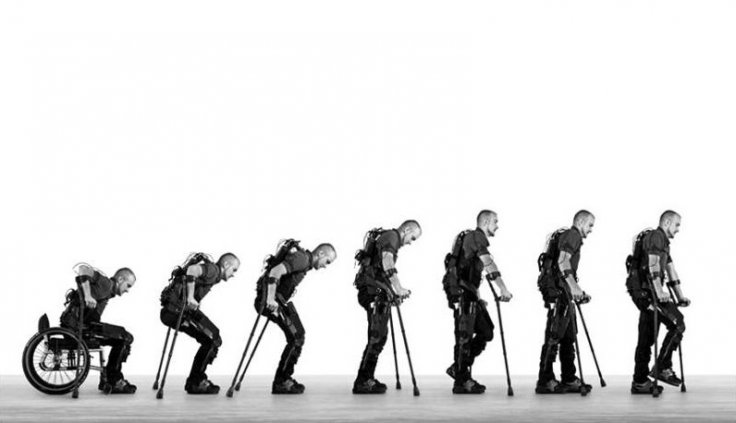
\includegraphics[width=\textwidth]{figures/Forside}
	\end{minipage}
	\hfill
\end{figure}

%\vspace*{\fill}
%\begin{center}
%	\textit{Gruppemedlemmer:}\\
%	Linette Helena Poulsen, Mads Kristensen, Maria Kaalund Kroustrup \\
%	Nirusha Jeevanandan \& Signe Hejgaard Kristoffersen
%\end{center}
\begin{center}
\line(1,0){400}
\end{center}

% Dette er LaTeX-versionen af titelbladet for TNB studenterrapporter
% Filen kræver:
% Universitetets logo:  AAU-logo-stud-UK eller AAU-logo-stud-DK
% Synopsis: En fil ved navn synopsis.tex

% Udarbejdet af: Jesper Nørgaard (jesper@noergaard.eu) 10. april 2012

\phantomsection
\pdfbookmark[0]{Titelblad}{titelblad}
\thispagestyle{empty}

\begin{minipage}[t]{0.48\textwidth}
\vspace*{-25pt}			%\vspace*{-9pt}

\includegraphics[height=4cm]{figures/AAU-logo-stud-DK-RGB}
\end{minipage}
\hfill
\begin{minipage}[t]{0.48\textwidth}
{\small 
\textbf{School of Medicine and Health}\\
Sundhedsteknologi \\
Fredrik Bajersvej 7A \\
9000 Aalborg \\
http://www.smh.aau.dk}
\end{minipage}

\vspace*{1cm}

\begin{minipage}[t]{0.48\textwidth}
\textbf{Titel} \\[5pt]\hspace*{2ex} 
Udvikling af et EMG-baseret \\\hspace*{2ex}
kontrolsystem til body \\\bigskip\hspace*{2ex}
augmentation-systemer 

\textbf{Projekt} \\[5pt]\bigskip\hspace*{2ex}
Behandling af fysiologiske signaler%\\\bigskip\hspace*{2ex} 

\textbf{Projektperiode} \\[5pt]\bigskip\hspace{2ex}
01-02-2016 - 27-05-2016

\textbf{Projektgruppe} \\[5pt]\bigskip\hspace{2ex}
16gr4405

\textbf{Gruppemedlemmer} \\[5pt]\hspace*{2ex}
Linette Helena Poulsen \\\hspace*{2ex}
Mads Kristensen \\\hspace*{2ex}
Maria Kaalund Kroustrup \\\hspace*{2ex}
Nirusha Jeevanandan \\\bigskip\hspace*{2ex}
Signe Hejgaard Kristoffersen %\\\bigskip\hspace{2ex}


\textbf{Vejleder} \\[5pt]\bigskip\hspace*{2ex}
Steffen Frahm %\\\bigskip\hspace{2ex}


\vspace*{1cm}

%\textbf{Oplagstal: } \\
\textbf{Antal sider: ???} \\
\textbf{Antal bilag: ???} \\ 
\textbf{Afleveret: 27-05-2016}

\end{minipage}
\hfill
\begin{minipage}[t]{0.483\textwidth}
\textbf{Synopsis} \\[5pt]
\fbox{\parbox{8cm}{\bigskip%Introduktion
The purpose of this project is to examine the possibility to control an exoskeleton during a squat exercise to support amyothrophic lateral sclerosis patients' muscles. This study consists of measurements from the muscle, rectus femoris, and two accelerometers. The muscle activity shows the patients movement during a squat. The inputs signals from the accelerometers are calculated to show the knee's angle. A digital has system has been designed, implemented and tested to evaluate the system. The study is based on grey literature, articles, books and tests which has been analyzed and interpreted. It is not possible to use the system to help the patients currently since the prototype has not been developed. The test of the system shows that it possible to detect whether the user is moving upwards or downwards during a squat exercise, when the angle of the knee is between $90^{\circ}$ og $180^{\circ}$, by analysing the input signals from the rectus femoris and the accelerometres. \bigskip}}
\end{minipage}

\vfill

{\footnotesize\itshape \noindent Rapportens indhold er frit tilgængeligt, men offentliggørelse (med kildeangivelse) må kun ske efter aftale med forfatterne.}

% Rapportens indhold er frit tilgængeligt, men offentliggørelse (med kildeangivelse) må kun ske efter aftale med forfatterne.
% The content of the report is freely available, but publication (with source reference) may only take place in agreement with the authors.

\chapter*{Forord}
Dette projekt er udarbejdet af gruppe 16gr4405, 4. semesters-studerende på Sundhedsteknologi, Aalborg Universitet. Projektet er udarbejdet i perioden mellem den 1. februar og den 27. maj 2016 og tager udgangspunkt i semestrets tema \textit{Behandling af fysiologiske signaler}. Yderligere er projektet udarbejdet på baggrund af projektforslaget \textit{Udvikling af et EMG-baseret kontrolsystem til body-augmentation systemer}. Ifølge studieordningen for Sundhedsteknologi på 4. semester har projektet følgende formål: \textit{"Med udgangspunkt i opnået viden, færdigheder og kompetencer på 3. semester arbejdes der med teori og metoder til opsamling og præsentation af signaler fra kroppen, men nu med fokus på digital signalbehandling og datakommunikation"}. \citep{aalborguniversitet2014}

Der rettes tak til vejleder Steffen Frahm for god vejledning og et godt samarbejde. Herudover rettes der tak til John Hansen for hjælp til datakommunikation samt programmering. 
\section*{Læsevejledning}
Projektrapporten er opdelt i 7 kapitler samt tilhørende bilag. Det første kapitel indeholder en indledning til projektet samt den initierende problemstilling. Andet kapitel består af problemanalysen, der er udarbejdet på baggrund af den initierende problemstilling. Problemanalysen leder op til en projektafgrænsning samt problemformulering. Fra tredje til sjette kapitel beskrives problemløsningen, der består af systemudvikling, løsningsstrategi, teori og design, implementering samt test af de enkelte blokke og det samlede system. Det syvende og sidste kapitel består af syntese, der indeholder en diskussion, konklusion samt perspektivering af projektet. Dette efterfølges af bilag samt litteraturlisten. 

I dette projekt anvendes Vancouver-metoden til refereringen af kilder. Kilderne referes som tal, der er omgivet af kantede parenteser. I litteraturlisten ses kilderne, der eksempelvis er angivet med forfatter, titel og årstal. Hvis kilden er angivet før et punktum, er der referet til den forrige sætning. Hvis kilden er angivet efter punktum, er der refereret til hele afsnittet. Forkortelser i rapporten er skrevet i en parentes første gang, hvorefter forkortelsen bliver anvendt i den resterende del af rapporten.
 
Denne projektrapport er udarbejdet i LaTex. Herudover er der anvendt MATLAB  til at visualisere diverse grafer. Yderligere er PSoC Creator anvendt til behandling af data samt programmering af systemet.  


\subsection*{Flowdiagram håndtering} \label{sec:flowhaandtering}
For at kunne forstå og læse flowdiagrammerne, som anvendes i projektet, forklares betydningen af de forskellige former. De forskellige former fremgår af \autoref{fig:flow}.

\begin{figure}[H]
\centering
\includegraphics[width=0.3\textwidth]{figures/flow}
\caption{Illustration af de anvendte former i flowcharts.}
\label{fig:flow}
\end{figure}

\noindent
Cirklen indikerer start og stop af funktion. Firkanten indikerer en beslutning. Diamant formen indikerer en midtvejs proces.
\clearpage

%%%% Indholdsfortegnelse (TOC) %%%%
\phantomsection													% Kunstigt afsnit, som hyperlinks kan 'holde fast i'
\pdfbookmark[0]{Indholdsfortegnelse}{indhold}					% Tildeler en klikbar bookmark til den endelige PDF
\tableofcontents*												% Indholdsfortegnelsen (kaldet ToC) 
%\clearpage
%\addtocontents{toc}{\protect\newpage}							% Fremtvinger sideskift i ToC hvis noedvendig (der hvor koden placeres)

\mainmatter

%Introduktion--------------------------------
%\chapter{Indledning}\label{Indledning}
% !TeX spellcheck = da_DK
\subsection{Indledning}
heuhkehhorho
\input{rapportAfsnit/bInitierende/initierende_spg}

%-----------------------Problemanalyse---------------------------
\chapter{Problemanalyse}
\section{Amyotrofisk lateral sklerose} \label{sec:ALS}
ALS er en neurodegenerativ sygdom, der påvirker motorneuronerne i hjernen, hjernestammen og rygsøjlen i takt med sygdommens fremskriden, hvilket resulterer i muskelsvaghed \citep{henschke2012}. 
En illustration af, hvordan ALS påvirker motorneuroner, illustreres på \autoref{fig:affectedneuron}. 
De første symptomer på sygdommen er kramper, svaghed samt stive muskler, hvilket kan opstå som muskelsvaghed i arme eller ben, talebesvær eller svaghed i de muskler, som styrer respirationen \citep{nationalinstitute2016}. 
Symptomer og følger af ALS varierer fra patient til patient, hvorved nogle patienter først oplever muskelsvaghed i deres ben, mens andre oplever muskelsvaghed i deres hænder og arme eller besvær ved tale- eller synkebesvær \citep{nationalinstitute2016, miller2005}.

\begin{figure}[H]
\centering
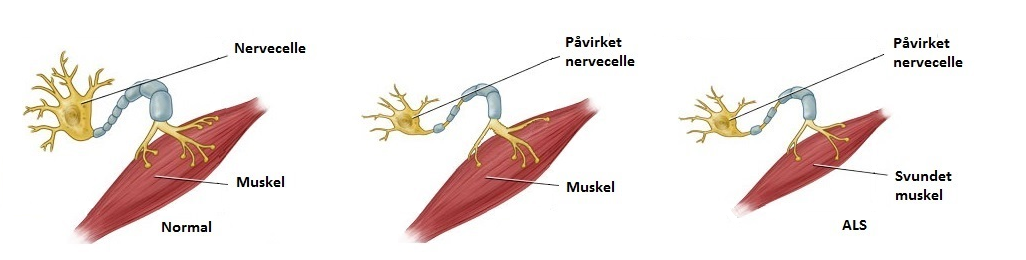
\includegraphics[width=1\textwidth]{figures/affectedneuron}
\caption{Nervecelle og muskel påvirket af ALS. Til venstre ses en normal motorneuron samt en upåvirket muskel. I midten fremgår motorneuronet påvirket af ALS, dog ses musklen endvidere upåvirket. Til højre ses motorneuronet påvirket, samt at musklen er svundet ind. Svindet skyldes en manglende stimulering af musklen som følge af den påvirkede motorneuron \citep{drake2015}.}
\label{fig:affectedneuron}
\end{figure}
 
\noindent
Muskelsvagheden skyldes abnormiteter i de nedre motorneuroner. De nedre motorneuroner er de nerveceller, der videregiver information fra rygmarven til musklerne. 
Symptomer på abnormiteter i de nedre motorneuroner ses som muskelsvaghed samt muskelkramper og atrofi.
Ligeledes kan de øvre motorneuroner påvirkes. Disse motorneuroner sørger for kommunikationen mellem hjernen og de nedre motorneuroner i rygmarven. 
Ved abnormitet, opstår komplikationer ved vidersendelse af beskeder til det givne sted. 
Dette ses som spasticitet samt overdrevne reflekser \citep{nationalinstitute2016}. Opdelingen af de nedre samt øvre motorneuroner ses på \autoref{fig:motorneuroner}.

\begin{figure}[H]
\centering
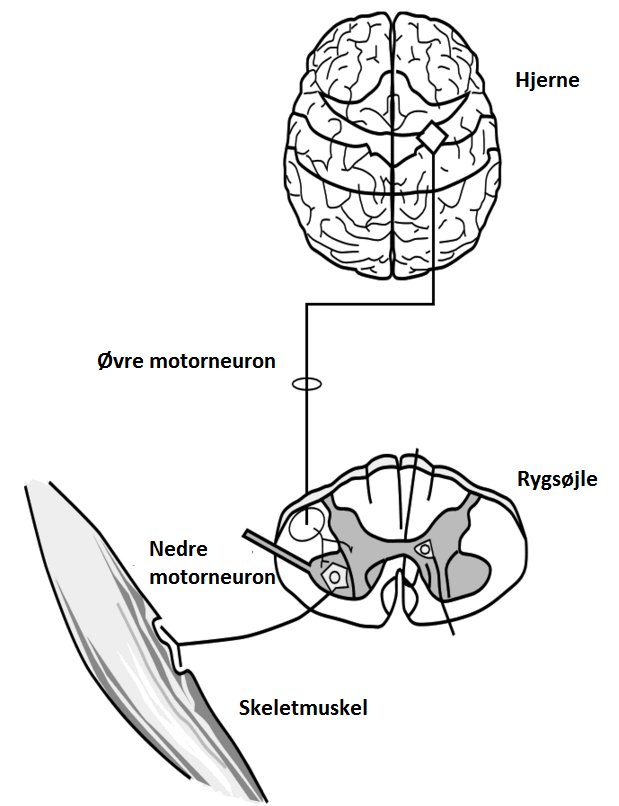
\includegraphics[width=0.6\textwidth]{figures/motorneuroner.png}
\caption{Illustrerer opdelingen af de nedre samt øvre motorneuroner i forhold til hjernen, rygsøjlen og skeletmuskulaturen \citep{miller2005}.}
\label{fig:motorneuroner}
\end{figure}

\noindent
Årsagen til ALS' opståen er oftest ukendt, dog ses en arvelighed i $5 - 10~\%$ af tilfældene. Heraf anslås, at $20~\%$ har det muterede Superocide dismutase 1-gen (SOD-1), hvilket resulterer i tab af motorneuroner \citep{miller2005}.

På trods af, at ALS opleves individuelt både i forhold til sygdomsprogressionen samt, hvilke komplikationer de oplever, kan sygdommen inddeles i tre stadier: et tidligt, midt og endeligt stadie. Et diagram af de tre stadier fremgår af \autoref{fig:stadier}.

\begin{figure}[H]
\centering
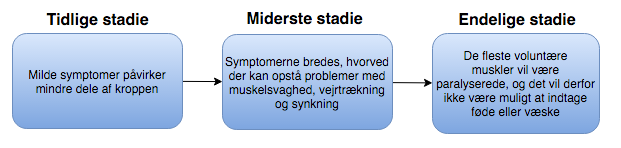
\includegraphics[width=1\textwidth]{figures/stadier.png}
\caption{Tre stadier for udviklingen af ALS samt de tilhørende symptomer.}
\label{fig:stadier}
\end{figure}

\noindent
I det tidlige stadie kan patienter overse symptomer på ALS, da disse er milde og kun påvirker mindre dele af kroppen \citep{themusculardystrophyassociation2016}. 
Ved det midterste stadie vil symptomerne udbrede sig, og nogle muskler paralyseres. Andre muskler vil blive svagere med tiden, hvilket blandt andet kan medføre problemer med synkning og vejrtrækningen \citep{themusculardystrophyassociation2016}. I det endelige stadie vil de fleste voluntære muskler være paralyserede, og det vil derfor forringe muligheden for selv at indtage føde eller væske. 
Herudover vil patienter oftest i dette stadie miste evnen til selv at trække vejret, og de bliver derfor afhængige af ventilationsstøtte \citep{themusculardystrophyassociation2016}.
Den mest almindelige dødsårsag er respirationssvigt, hvilket oftest sker inden for tre til fem år efter diagnosen er stillet \citep{morris2015}. $25~\%$ af patienterne har en overlevelsesrate på fem år, og kun $10~\%$ lever længere end ti år efter diagnosen er stillet \citep{grehl2011, miller2005}.


%Til at starte med kan mindre symptomer som besvær ved at gå op ad trapper opstå. Ligeledes kan patienterne være påvirket af dropfod, når de går. Herefter vil musklerne gradvist blive svagere, og med tiden vil patienterne ikke længere være i stand til at gå.\citep{tidy2015} 
%\section{Følger}

ALS er en individuel sygdom og sygdommens forløb vil ligeledes variere fra patient til patient. Dog kan der være fællestræk for sygdommens progression, men med undtagelse af nogle patienter. Man kan inddele sygdommen i 3 stadier, et tidligt stadie, et mellem stadie og et sent stadie. I de tidligste stadier er der mulighed for, at patienterne kan ignorere symptomerne og diagnosticeres oftest efter dette stadie. [1] Disse symptomer kan være milde og kun påvirke mindre dele af kroppen, hvor musklerne eksempelvis kan være svage eller stive. Dette vil ligeledes have påvirkning på patientens balance. I det midterste stadie vil symptomerne begynde at udbrede sig. Nogle muskler kan være paralyserede, hvor andre eksempelvis kan være upåvirkede. Andre muskler vil blive svagere med tiden og dette vil blandt andet medføre problemer med synkning og vejrtrækningen. I de senere stadier vil de fleste voluntære muskler vil være paralyserede og det vil måske ikke være muligt at indtage føde eller væske. Herudover vil det for oftest i dette stadie ikke være muligt at trække vejret grundet respirationssvigt. [1] 

Symptomerne behøver nødvendigvis ikke at ramme begge ben samtidig. Til at starte med at mindre symptomer som besvær ved at gå op ad trapper. Ligeledes kan det være patienterne vil begynde at være nødsaget til at trække benet for at kunne gå. Herefter vil det musklerne gradvist blive svagere og med tiden vil de ikke længere være i stand til at gå. [2]



1: https://www.mda.org/disease/amyotrophic-lateral-sclerosis/signs-and-symptoms/stages-of-als 
2: http://patient.info/health/motor-neurone-disease-leaflet 
 Denne skal ikke være med i master dokumentet. 
\subsection{Livskvalitet hos ALS-patienter}
% mere konkret omkring deres livskvalitet og familieforhold
% tilføj tabel 2 fra ilse2015
Livskvaliteten hos patienter med ALS undersøges for at vurdere, hvilken påvirkning sygdommen samt dens progression har på patienten. Der er ingen behandling for at stoppe sygdomsprogressionen, men der eksisterer forskellige palliatative behandlinger. Det er fordelagtigt at kende patienternes livskvalitet for at vurdere den optimale palliative behandling. \citep{neudert2004,ilse2015}

Livskvalitet defineres ud fra en persons fysiske sundhed, psykologiske tilstand, grad af selvstændighed, sociale relationer og personlig tro. \citep{pagnini2013}

Der kan fremhæves to forskellige typer af livskvalitetsvurderinger: en overordnet liskvalitet og en sundhedshedsrelateret livskvalitet. 
Den overordnede livskvalitet relaterer til patienternes samlede livskvalitet, og den sundhedsrelaterede livskvalitet dækker over de fysiologiske og mentale aspekter ved sygdommen. \citep{ilse2015, nuebert2004} Da ALS påvirker patienters fysiske formåen, ses der et fald i denne type livskvalitet, som sygdommen fremskrider. \citep{ilse2015} Dette fremgår også af \autoref{livskvalitet}, som viser en forringet livskvalitet hos ALS-patienter når der sammenlignes med resten af befolkningen. Livskvaliteten vurderes ud fra mobilitet, selvpleje, udførelse af normale aktiviteter, oplevelse af smerte eller ubehag samt diagnoser som angst og depression, hvor næsten 3 gange så mange ALS-patienter lever med disse problemer sammenlignet med den resterende befolkning.

\begin{table}[H]
\centering
\label{livskvalitet}
\begin{tabular}{l| l| l}
\multicolumn{3}{c}{\textbf{Moderate eller alvorlige problemer målt ud fra europæisk livskvalitetsvurdering}}
   \\
                                                                         & ALS-patienter                                    & Normativ tysk population                                   \\
Mobilitet                                                                & 83,7 \%                                          & 16,6 \%                                                    \\
Selvpleje                                                                & 77, 6 \%                                         & 2,9 \%                                                     \\
Normale aktiviteter                                                      & 85,7 \%                                          & 10,2 \%                                                    \\
Smerte eller ubehag                                                      & 61,2 \%                                          & 27,9 \%                                                    \\
Angst eller depression                                                   & 67,4 \%                                          & 4,4 \%                                                    \\
\end{tabular}
\caption{sammenligner livskvaliteten for ALS-patienter med livskvaliteten for den tyske population. Det ses heraf at ALS-patienter har en forringet livskvalitet i forhold til den resterende tyske befolkning.\citep{ilse2015} (Revideret)}
\end{table}

\noindent
Til trods for, at der sker et fald i den sundhedsrelaterede livskvalitet, er der tidligere vist, at den overordnede livskvalitet forbliver stabil \citep{ilse2015, nuebert2004}. Dette kan forklares ved et "response shift" eller "frame shift", der er en måde at håndtere sin sygdom, hvor social støtte under sygdomsforløbet vægtes højere end normalt i bestemmelsen af livskvalitet. \citep{ilse2015} Af denne grund foreslås det, at faldet i sundhedsrelateret livskvalitet i forhold til mobilitet og selvhjælp afhjælpes ved teknologiske hjælpemidler. På denne måde vil ALS-patienternes sociale interaktioner kunne have fokus på deres sociale netværk, da disse sociale interaktioner er begrænsede på baggrund af ALS. \citep{ilse2015,tramonti2012}







% Jeg ved ikke, om dette er nok. Men jeg tænker, at vinklingen er mere som den, vi snakkede om. Der kan sandsynligvis sagtens tilføjes noget hertil - evt. tænker jeg, om man vil kunne tilføje (noget af?) tabel 2 fra ilse2015 for at få nogle tal på bordet. 
% Mads: Det er min hensigt at lave en form for afgrænsning til de fysiske mangler ved at tage udgangspunkt i den sundhedsrelateret livskvalitet og det med at den forringes i takt med at de oplever større svaghed i musklerne. 
%Tænker det er en afgrænsning vi bliver nød til at fortages os, for jeg synes ikke at kunne finde litteratur der giver den nødvendige relation mellem det at jeg skal fokusere på besværligheden i at gå.
% !TeX spellcheck = da_DK
\subsection{Nuværende teknologier/hjælpemidler}
% Da der ikke er nogen bevis kur for ALS er teknologierne er pallialiv, dvs. at den er lindrende. 
Som tidligere nævnt er ALS en livstruende sygdom, hvor følgerne sker gradvist, hvilket gør at patienternes funktionelle evner svækkes over sigt, hvorfor der er behov for en række hjælpemidler som helt eller delvist kan være en hjælp i hverdagen. Nogle af hjælpemidlerne er i starten af sygdommen for at patienterne kan klare sig selvstændigt, hvor der senere er behov for andre hjælpemidler samt helt eller delvist hjælp fra en ægtefælde eller plejepersonale. Der anvendes på nuværende tidspunkt teknologiske og personlige hjælpemidler. [2]

\subsubsection{Teknologiske og personlige hjælpemidler}
De mest anvendte hjælpemidler for patienter med ALS er teknologiske som f.eks.  kørestole, toiletstole og stokke. Hjælpemidlerne er alle redskaber som støtter og aflaster patienten. Derudover anvendes der mere personlige hjælpemidler som i stedet er tilpasset patienterne individuelt. Patienterne har på denne måde et særligt behov for hjælpemidler som f.eks. tilpasset kørestole, tilpasset fodtøj og høreapparat. [2]

\subsubsection{Udfordringer og muligheder}
\fxnote{På nuværende tidspunkt har det være svært at finde nogle kilder i forhold til muskelsvind og det at gå, men mine tanker er noget med at koble det sammen ift. det der står under livskvalitet og de nuværende teknologier der er hvor lidt selvstændighed det giver i hverdagen og så senere koble det til at kunne anvendes exoskelet........}
Der er ingen af de nuværende teknologier som giver patienten mulighed for at gå, men hvis patienterne har gangbesvær vil de kunne anvende hjælpemidler som stok og rollator, ellers vil de være nødsaget til at anvende en kørestol for at kunne komme fra A til B. hvilket i forhold til livskvalitet bla..bla..blaa.. er patienterne gerne vil gå.


\subsubsection{Løsning}
Exoskelet som har til opgave at......




Det er her udover påvist at flere af disse metoder ud fra patienternes vurdering medvirker til en forbedret livskvalitet [1]

%[1] http://www.tandfonline.com.zorac.aub.aau.dk/doi/pdf/10.1080/00222895.2014.891970
%[2] https://books.google.dk/books?id=ha23lFiOGX8C&printsec=frontcover&hl=da&source=gbs_vpt_buy#v=onepage&q&f=false Grundbog om hjælpemidler - til personer med funktionsnedsættelse Åse brandt og lilly Jensen  
% !TeX spellcheck = da_DK
\section{Gangfunktion}
Efterhånden som ALS-patienter mister muskelkraft, vil bevægeligheden i deres led nedsættes. Af denne grund opstår der kontrakturer i led, og muskelstramninger i de omkringliggende muskler.

Ved gang anvendes knæ-, hofte- og ankelleddet, hvilket fremgår af \autoref{fig:knaet}, hvis disse led ikke akviteres, opstår der muskelstramninger i benene \citep{instforms2008}.

\begin{figure} [H]
\centering
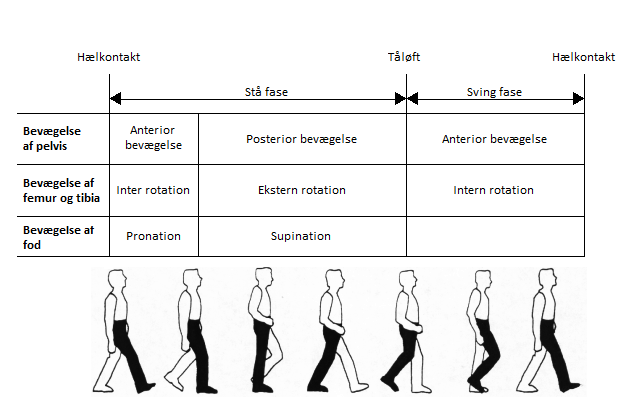
\includegraphics[width=0.9\textwidth]{figures/knaet}
\caption{Viser bevægelse af pelvis, femur og tibia samt foden ved forskellige faser under gang \citep{orthopedics2016}.}
\label{fig:knaet}
\end{figure} 

\noindent
Knæleddet vælges som udgangspunkt for et muligt body augmentation-system i form af et exoskelet, da knæleddet er et hængselled og derfor har et begrænset antal frihedsgrader. Knæleddet har én frihedsgrad, modsat andre mere komplekse led, hvilket gør, at leddet kun kan bevæge sig i én akse \citep{martini2012}. 
Det antages derfor, at knæleddet er et af de led, som er simplest at opbygge et system omkring. 
Hvis der kan laves et exoskelet omkring knæleddet, vil det kunne antages, at samme princip kan muliggøres ved henholdsvis hofte- og ankelleddet, hvorved gangfunktionen kan opretholdes.

\subsection{Knæets opbygning}
Knæet består af tre separate ledforbindelser. To, der er forbundet mellem femur og tibia, samt en mellem patella og femur, hvilket fremgår af \autoref{fig:knae_anatomi}. 

\begin{figure}[H]
\centering
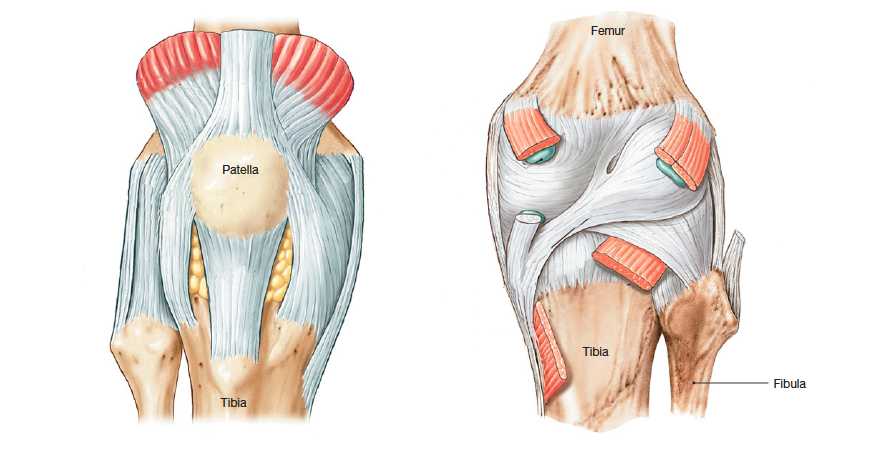
\includegraphics[width=0.8\textwidth]{figures/knae_anatomi}
\caption{Knæets anatomiske opbygning samt knæets forreste og bagerste korsbånd. \citep{aaos2014}.}
\label{fig:knae_anatomi}
\end{figure} 

\noindent
Ud over de tre separate ledforbindelser stabiliseres knæet af syv ledbånd. Ét af de syv ledbånd er patellarsenen, som er ansvarlig under extension af knæet. Derudover strækker to ledbånd sig mellem femur, tibia og fibia, hvilket er med til at styrke knæleddets overflade posteriort. 
Inde i ledkapslen befinder det forreste korsbånd, Anterior Cruciate Ligament (ACL), og det bagerste korsbånd, Posteior cruciate ligament (PCL), sig. Disse har til opgave at fastgøre indre knoglefremspring af tibia til knoglefremspringet på femur. 
Korsbåndene har til opgave at begrænse anteriore og posteriore bevægelser af femur og er med til at opretholde retningen af knoglefremspringene. 
Det tibiale kollaterale ligament forstærker den mediale flade af knæleddet, og det fibulære kollaterale ligament forstærker sidefladen. Disse ligamenter anvendes kun ved fuld ekstension af knæleddet \citep{martini2012}.

\subsection{Knæets funktion}
Ved gang aktiveres quadricepsmusklerne, der sidder anteriort på femur, og hasemusklerne, der sidder poseriort på femur. Nogle af disse muskler fremgår af \autoref{fig:laarmuskler}. Quadricepsmusklerne består af rectus femoris, vastus intermedius, vastus medialis og vastus lateralis. 
Hasemusklerne består af biceps femoris, semitendinosus og semimembranosus. 
Ved bevægelse foretager quadriceps- eller hasemusklerne ekstension eller fleksion, hvorved de fungerer som hinandens agonister eller antagonister under bevægelse \citep{martini2012}. 

\begin{figure} [H]
\centering
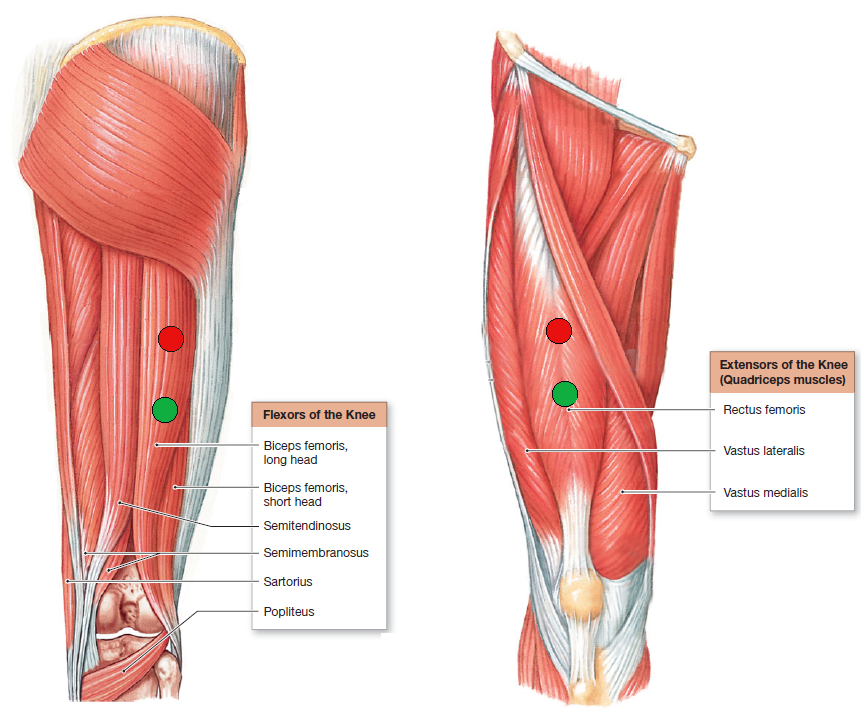
\includegraphics[width=0.9\textwidth]{figures/laarmuskler}
\caption{Viser rectus femoris, vastus lateris, biceps femoris, semimembranosus og patella  \citep{martini2012}.}
\label{fig:knaet}
\end{figure} 


Som tidligere nævnt anvendes hofte, knæ og ankler under gang. Udover disse led er kropsposituren og sving af leddene afgørende for gangfunktionen. Det fremgår af \autoref{fig:knaet}, hvordan de forskellige led udfører fleksion, ekstension og ændres fra ekstension til neutral bevægelse under gang \citep{martini2012}.

\subsubsection{Knæets funktion under en squat-øvelse} \label{sec:knaeled_squat}
% mere om, at det kun er lårets muskulatur, der benyttes under squat
Den dynamiske squat-øvelse er en udbredt træningsøvelse, som kræver styrke i flere muskelregioner. Squat aktiverer primært hofte-, lår- og rygmuskulaturen, som alle er primære muskler under gang, løb, spring og løft. Herudover anvendes squat som et redskab til rehabilitering af knæet, hvilket skyldes den måde, som knæet belastes under squat \citep{escamilla2001}. 

Knæets funktion for bøjningen af benet kan dermed ses ved udførelse af en squat-øvelse. En squat-øvelse udføres ved at stå i en oprejst position med knæ og hofte fuldt udstrakt. Herefter udføres en squat-øvelse i en kontinuerlig bevægelse, indtil den ønskede dybde nåes, hvorefter der udføres en kontinuerlig bevægelse tilbage til oprejst position \citep{escamilla2001}. En illustation af en squat-øvelse ses på \autoref{fig:squat}.

\begin{figure}[H]
\centering
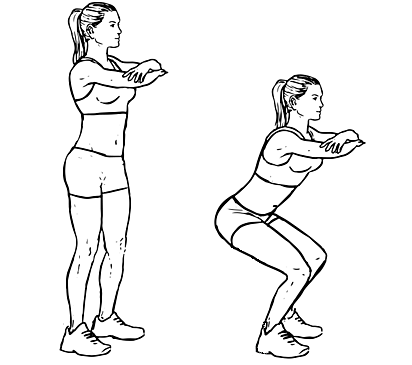
\includegraphics[width=0.5\textwidth]{figures/squat.png}
\caption{En illustration af udførelse af en halv squat-øvelse. Til venstre ses udgangspositionen, og til højre ses en halv squat-øvelse \citep{squat2015}.}
\label{fig:squat}
\end{figure}

\noindent 
Squat-øvelser kan udføres med varierende fleksion af knæet. De mest anvendte varianter af øvelsen er halv eller fuld squat. En halv squat-øvelse udføres indtil lårene er parallelle med jorden, hvilket svarer til en fleksion af knæet fra omkring $90-180^{\circ}$. En fuld squat-øvelse udføres indtil det posteriore del af låret og læggen kommer i kontakt med hinanden. Den fulde squat-øvelse anbefales mere trænede personer, hvorfor den halve squat-øvelse typisk er foretrukket til genoptræning af knæet \citep{escamilla2001}.

Ved udførelse af en squat-øvelse aktiveres blandt andet musklen rectus femoris. Aktiviteten i rectus femoris, og de resterende quadricepsmuskler, er størst ved $90-100^{\circ}$ vinkel af knæleddet \citep{schoenfeld2010}. 
Fra udgangspositionen for squat-øvelsen, der illustreres på \autoref{fig:squat}, befinder personen i en oprejst posistion med en vinkel på $180^{\circ}$ over knæet. Ved udførelse af en squat-øvelse vil muskelaktiviteten i rectus femoris være progressivt stigende indtil en vinkel over knæet på $90-100^{\circ}$ opnås. Idet der returneres til udgangspositionen, vil muskelaktiviteten være progressivt faldende \citep{escamilla2001}. 

%Biceps femoris aktiveres ved en $45^{\circ}$ fleksion af knæleddet, mens rectus femoris aktiveres ved en $80-90^{\circ}$ fleksion, hvorefter aktiviteten i musklerne er konsistent \citep{schoenfeld2010}. 


%Under en squat-øvelse aktiveres vastus intermedius, vastus medialis samt vastus lateris mere, da disse muskler er én ledmuskel, end rectus femoris der er en to-ledsmuskel \fxnote{hvorfor aktiveres én-ledsmuskler mere end to-ledsmuskler - jeg kan ikke finde det med hasemusklerne i den kilde der står til afsnittet?}.
%der er forbundet mellem femur, tibia og patella. Knæet har fire ledbånd. To af disse er side-ligamenterne, der sidder omkring knæleddet. De resterende to er korsbåndene, der sidder på skrå inden i knæet.
%Knæet fire ledbånd sikrer stabilisering af knæet og sørger for at knoglerne bevæger sig rigtigt.  Det er knæleddet, der gør det muligt for kroppen at kunne udføre aktiviteter som at kunne gå, løbe, og eksempelvis squatte. Ved gang aktiveres både quadriceps musklerne (rectus femoris, vastus intermedius, vastus medialis, vastus lateralis) der sidder anteriort for låret samt hamstring musklerne (biceps femoris, semitendinosus, Semimembranosus), der sidder posteriort for låret og kontraherer med quadriceps musklerne. 


% !TeX spellcheck = da_DK
\subsection{Problemafgrænsning}
I dette projekt fokuseres der på ALS patienter samt muligheden for opretholdelse af kropsfunktioner ved benyttelse af body augmentations hjælpemidler. 

Da ALS patienter oplever progressiv svind af deres muskler, har dette indflydelse på deres selvstændighed, da de bl.a. gradvist mister kontrollen over deres legemesdele. Da der kun eksisterer palliative behandlinger til ALS patienter fokuseres der på at afhjælpe deres fysiske mangel ved brug af et exoskelet som aflastning. Dette system kræver minimal fysisk indstat at anvende, hvilket er passende til den typiske ALS patient. 
Ved opretholdes af de fysiske funktioner vil dette ligeledes have en positiv effekt på den sundhedsrelateret livskvalitet, da dette vil kunne resultere i en større selvstændighed. Der er dog igen garanti på at det vil gavne den overordnede livskvalitet hos ALS patienten.  

Idet ALS vil resultere i, at patienten mister evnen til at kunne gå, fokuseres der på at opretholde denne funktion. Til dette er det fremhævet, at knæet er det vigtigste led i forhold til at kunne gå. Dertil vælges der at tages udgangspunkt i knæleddet, hvor musklerne omkringliggende knæet afhjælpes ved anvendelse af et exoskelet.

\subsection{Problemformulering}
Hvordan kan et exoskelet anvendes over et knæled, med henblik på, at ALS patienter skal opretholde deres evne til at gå 

%%-----------------------System udvikling-------------------------
\chapter{Systemudvikling} 
\section{Systembeskrivelse}
Der ønskes, som tidligere nævnt, at udvikle et system, der har til formål at aflaste musklerne omkring knæleddet under udførelse af en statisk squat-bevægelse ved brug af et exoskelet. Dette gøres for at aflaste patienterne med henblik på at kunne undgå kørestol i tidlige stadier af ALS. Systemet skal kunne opsamle signaler fra lårmusklerne; quadriceps og hamstring. Disse signaler skal behandles og omsættes til aktivitet i en prototype af et exoskelet, som skal udføre en tilsvarende bevægelse, men også have mulighed for forstærkning af signalet, så mindre muskelkraft også vil kunne udløse denne bevægelse. Ud over aktiviteten i musklerne skal exoskelettet kunne begrænse bevægelse i visse retninger, så det herved er muligt at rette leddets position, hvis dette bevæger sig uønsket\fxnote{har vi snakket om dette?}. Af denne grund skal systemet være i stand til at måle muskelaktivitet i quadriceps og hamstring samt den aktuelle vinkel i knæleddet. Derudover skal systemet være brugervenligt ved at være kompakt, mobilt og ikke generende over for brugeren.

\subsection{Krav til systemet} 
\begin{itemize}
\item Systemet skal registrere muskelaktivitet og ledvinkler
\item Systemet skal kunne overføre data trådløst til en computer
\item Systemet skal kunne udmundes(bedre ord?) i en prototype af et exoskelet
\item Systemet skal være batteridrevet
\item Systemet skal være sikkert og ikke til gene for brugeren
\item Systemet skal kunne indikere, hvis der ikke er strøm nok til at virke optimalt \fxnote{er dette et vigtigt punkt?}
\item Systemet skal kunne give feedback og derved sørge for, at brugeren befinder sig inden for følgende specifikationer:\fxnote{igen: har vi snakket om dette?}
\begin{itemize}
\item XX antal grader?
\item XX antal grader?
\end{itemize}
\end{itemize}

\fxnote{Punkterne står virkelig tæt på teksten - kan vi ændre på det?}

\subsection{Blokdiagram}\fxnote{ændr feedback til prototype, tilføj måske patienten}
\begin{figure}[H]
\centering
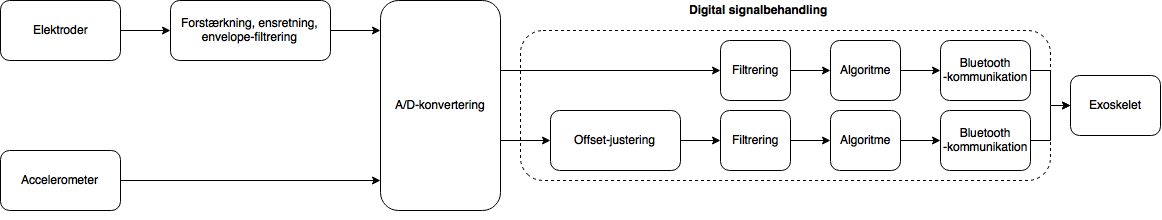
\includegraphics[width=0.4\textwidth]{figures/blokdiagram.png}
\caption{Systemets opbygning.}
\label{fig:blokdiagram}
\end{figure}

%I dette projekt er der valgt at udarbejde en prototype, som har til formål at sørge for at knæledddet forbliver inden for en bestemt position. 
I dette projekt er der valgt at udarbejde en prototype, som har til formål at bøje knæleddet, når lårets muskler kontraherer. Opbygningen af systemet fremgår af \autoref{fig:blokdiagram}. Der anvendes to sensorer, EMG og accelerometer, til at opsamle biologiske signaler, For at registrere muskelaktivitet anvendes en EMG-sensor og en EMG-forstærker, der har til formål at forstærke den muskelaktivitet, der opsamles. Accelerometeret anvendes for at give systemet et input om, knæleddet vinkles  under udøvelsen af en statisk squat. Det opsamlede signal sendes herefter videre til den digitale del af systemet, hvilket er bestående af et Bluetooth Low Energy Pioneer kit (CY8CKIT-042-BLE), som opfanger de biologiske signaler og overfører dem trådløst til en CySmartUSB BLE Dongle sat i en computer, som kan kommunikere med prototypen af exoskelettet i LEGO Mindstorms. 



%%\subsection{Elektromyografi}
%EMG er en målemetode, som måler elektrisk aktivitet genereret af musklerne \citep{chowdhury2013}. 
%En EMG-måling dækker over et samlet antal potentialer fra måleområdet, idet der aktiveres mange muskelfibre \citep{keenan2012}. \fxnote{Ved ikke, om der skal skrives noget om, at muskelfiberne inaverers af motorneuroner, og at mængden af muskelfibre pr. motorneuron afhænger af musklen og dens funktion = det ville være godt, inddrag lidt ALS - KOMMENTAR: lige nu syntes vi ikke at der er relevant}

%Der kan anvendes to forskellige typer af EMG-målinger. Den ene er en ikke-invasiv metode, der kaldes overflade-EMG, og den anden er en invasiv metode, intramuskulær EMG \citep{chowdhury2013, keenan2012}. Hertil anvendes sidstnævnte i dette projekt. 
%Ved generel anvendelse af EMG-målinger, benyttes frekvensområdet ved $10-500~Hz$, hvorfor signaler uden for dette frekvensområde kan betegnes som støj \citep{morre2003, keenan2012}.  

%Denne metode kan påvirkes af flere artefakter, som bevægelsespåvirkning og støjpåvirkning fra elnettet ($50~Hz$) \citep{keenan2012}.
%Ligeledes kan der ved EMG-målinger fremkomme elektrisk støjpåvirkning fra omkringliggende muskler i forhold til området, der måles på. Dette betegnes som crosstalk \citep{keenan2012}. 

\subsection{Elektromyografi}
Til behandling af EMG-signalet, anvendes Muscle Sensor V3, der fremover refereres som 'EMG-forstærker'. Denne komponent måler en differens af de elektriske potentialer der måles gennem elektroderne. EMG-forstærkeren overholder de opstillede krav, og kan anvendes direkte med mikrokontrolleren. EMG-forstærkeren består af en intrumenteringsforstærker, et passivt højpasfilter, en full-wave rectifier, et aktivt lavpass filter og en justerbar forstærker \citep{advancertech2013}. 

En illustration af, hvordan EMG-forstærkeren behandler et inputsignal fremgår af \autoref{fig:sinussignal}.
\begin{figure}[H]
\centering
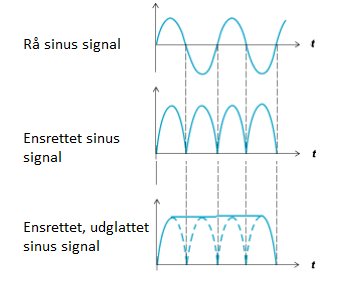
\includegraphics[width=0.6\textwidth]{figures/sinussignal.png}
\caption{Tre sinussignaler. Henholdsvis et råt, ensrettet og ensrettet samt udglattet. \citep{advancertech2013}.}
\label{fig:sinussignal}
\end{figure}

Med udgangspunkt i \autoref{fig:sinussignal} ses signalet som sinuskurven. Hertil passerer det højpasfilteret der dæmper DC støjen og dermed offsettet i signalet. Dette ses som signalet sinuskurven der svinger omkring 0, og er nødvendig for at ensretningen viker efter hensigten. Dernæst ensrettes signalet, således de negative værdier inverteres, og at der kun er svingninger i positiv retning. Herefter fortages et envalope, hvilket ses som det udglattede signal, hvortil der er beregnet en knækfrekvens på $1,94~Hz$, ud fra \autoref{eq:lavcutfre}. 

\begin{equation}\label{eq:lavcutfre}
f_c = \frac{1}{2 \pi C R} = \frac{1}{2 \pi \dot 1 \dot 10^{-6}F \dot 80,6 \dot 10^3\Omega} = 1,94~Hz
\end{equation}

EMG-forstærkeren har en minimum spændingsforsyning på $\pm 3~V$ samt en maksimal spændingsforsyning på $\pm 30~V$. Herudover er der mulighed for at justere gain med en faktor fra 0,002 til 20,700. \citep{advancertech2013}. 





%Synes ikke det passer ind her? Er det ikke meningen dette skal være mere overordnet, og så specificerer vi os senere til hvordan vi vil måle, sådan til vores forsøg?
%Den ene elektrode placeres over enten rectus femoris eller vastus intermedius (sidder under rectus femoris) og den anden elektrode placeres over biceps femoris. Reference elektroden placeres ved??.. 


%Støj kan reduceres ved at placere en 0.1 mikro f capacitor i nærheden, det er dog nødvendigt at tilføje mere, hvis der er 50 KHz støj, da det vil kunne resultere i fejl i accelerations målingen. Støjens tæthed vil forminskes i takt med at forsyningsspændingen forøges.
%Fase sensitiv demodulation teknikker er anvendt for at bestemme magnituden samt accelerationens retning. Demodulator outputtet er forstærket og bragt igennem en 32 k ohm modstand. – noget med det forebygger aliasing 
%  - Jeg ser dette som 'ligegyldigt' nu, da det handler om kondensator og støj. Kan ikke se hvorfor det skal bruges (endnu) måske skal det bruges efter vi har lavet pilotforsøg, hvis der viser sig meget støj






%\subsection{Accelerometer}
Et accelerometer er en elektromekanisk enhed, som både kan måle statisk og dynamisk accerleration. Den statiske acceleration kan være tyngdekraften, hvortil det er muligt at bestemme orienteringen af accelerometeret i forhold til jorden. De dynamiske kræfter såsom bevægelse, stød og vibrationer, gør det muligt at analysere accelerometeres bevægelse samt hastighed. 

I dette projekt anvendes accelerometeret ADXL335Z, som har pin konfigurationen, som kan ses på \autoref{fig:acc_pin}. Accelerometeret er en 3-aksialt sensor, som har et arbejdsområde på minimum $\pm$ $3~g$, og et output som spænding. Det analoge output signal er proportionelle med accelerationen \citep{analogdevices2010}. 


\begin{figure}[H]
\centering
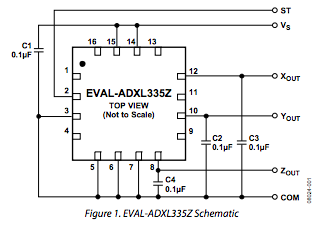
\includegraphics[width=0.6\textwidth]{figures/acc_pin.png}
\caption{Pin konfiguration af accelerometer ADXL335}
\label{fig:acc_pin}
\end{figure}

\noindent
Accelerometeret har en single-supply spændingsforsyning, som ligger mellem $1,8 - 3,6~V$, denne er reguleret til $XX~V$ via tilkobling af en regulator \fxnote{afhænger af hvad Jan sætter regulatoren til}. Offsettet er afhængig efter spændingsforsyningen, men ligger ved $XX~V$ på $XX~V$, denne beregnes som det halve af spændingsforsyningen. Båndbredden og støjen varierer for akserne. For x og y-aksen ligger båndbredden mellem $0,5 - 1.600~Hz$ og støjen normalt på $150~\mu g/\sqrt{Hz}$ RMS, mens båndbredden for z-aksen ligger mellem $0,5 - 550~Hz$ og støjen normalt på $300~\mu g/\sqrt{Hz}$ RMS. \fxnote{Den spektrale effekttæthed måles i $\mu g/$ og dividere dette med kvadratroden for båndbredden for signalet $\sqrt{Hz}$, hvilket giver RMS af accelerationsstøjen ved en temperatur på $25^\circ$C}. 

Da accelerometeret er ratiometrisk, hvilket vil sige at outputtet er direkte propotienelt med input, afhænger sensitiviteten ligesom offsettet af spændingsforsyningen. Ved $XX~V$ spændingsforsyning, ligger forsyningen på $XX~mV/g$ med en tolerance på $XX~\%$, hvor outputimpedansen er $XX~K\omega$ med en afvigelse på $XX~\%$. 

\begin{figure}[H]
\centering
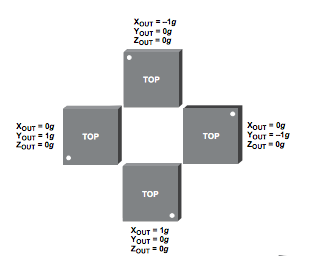
\includegraphics[width=0.8\textwidth]{figures/acc.png}
\caption{Accelerometeret, ADXL335Z, påvirkning i de forskellige akser}
\label{fig:acc}
\end{figure}

\noindent
Ved hældning af accelerometeret vil der ske en acceleration i forhold til tyngdekraften, afhængig af planet samt retningen som det hældes i. Dette fremgår af \autoref{fig:acc}. Herved vil der ske en ændring i spændingen fra referencepunkt ved en hældning på $0^{\circ}$\fxnote{Jeg forstår ikke den her sætning}. Hvis accelerometeret eksempelvis befinder sig i den øverste situation på \autoref{fig:acc}, påvirkes x-aksen med $-1~g$. Denne sammenhæng og derved patientens hældning kan udtrykkes ved følgende ligning:

\begin{equation}
	V_{out} = V_{offset} + sensitiviteten \cdot \sin(vinklen) \\
\end{equation}


%Støj kan reduceres ved at placere en 0.1 mikro f capacitor i nærheden, det er dog nødvendigt at tilføje mere, hvis der er 50 KHz støj, da det vil kunne resultere i fejl i accelerations målingen. Støjens tæthed vil forminskes i takt med at forsyningsspændingen forøges.
%Fase sensitiv demodulation teknikker er anvendt for at bestemme magnituden samt accelerationens retning. Demodulator outputtet er forstærket og bragt igennem en 32 k ohm modstand. – noget med det forebygger aliasing 
%  - Jeg ser dette som 'ligegyldigt' nu, da det handler om kondensator og støj. Kan ikke se hvorfor det skal bruges (endnu) måske skal det bruges efter vi har lavet pilotforsøg, hvis der viser sig meget støj
\section{Løsningsstrategi}
%Intro til hvad der skal være hjernen i systemet.
Til dette system benyttes komponenter fra Cypress's CY8CKIT-042-BLE udviklingssæt. 
Ud fra dette sæt er der udvalgt de nødvendige komponenter, så der kan fortages analog til digital konvertering af de signaler, der måles via sensorerne i \autoref{sec:sensorer}. Yderligere skal systemet være i stand til at kommunikere trådløst med andre enheder.   

\begin{figure}[H]
\centering
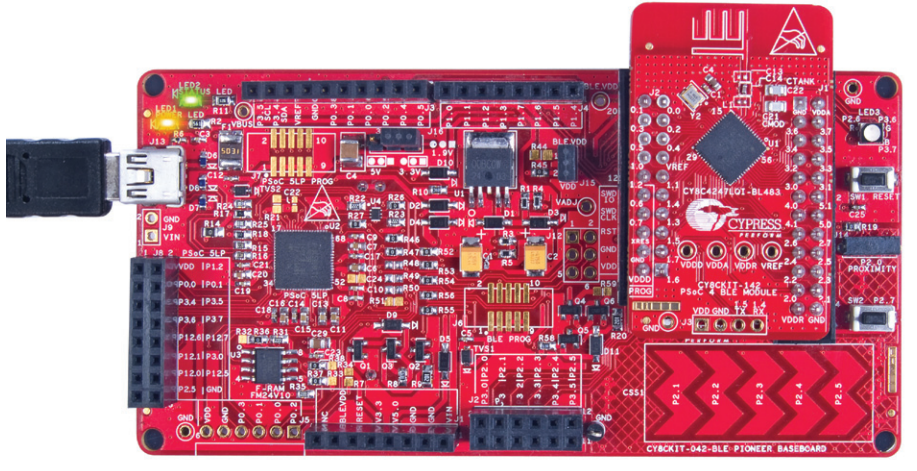
\includegraphics[width=0.5\textwidth]{figures/CY8CKIT-042.png}
\caption{CY8CKIT-042 BLE Pioneer baseboard, samt CY8CKIT-142 PSoC 4 BLE modulet \citep{cypresspsoc2015}.}
\label{fig:CY8CKIT-042}
\end{figure}

I \autoref{fig:CY8CKIT-042}, ses de valgte komponenter, der består af et CY8CKIT-042 BLE Pioneer baseboard og et CY8CKIT-142 PSoC 4 BLE modul. Baseboardet er platformen, hvorpå sensorerne vil blive tilkoblet, og hvor de analoge signaler konverteres til digitale signaler. Baseboardet har mulighed for tilkobling af en spændingsforsyning, bestående af et $3~V$ knapcelle batteri, eller via mikro USB tilslutningen \citep{cypressguide2014}. Der er mulighed for udvidelse af baseboardet, ved anvendelse af moduler fra Cypress, samt Arduino shields eller 6-pins Digilent Pmod udvidelseskort \citep{cypressguide2014}. 
\\


\subsection{Analog til digital konvertering}


\subsection{Trådløs kommunikation}
For at kunne kommunikere trådløst benyttes CY8CKIT-142 PSoC 4 BLE, der et Cypress BLE modul. Kommunikationstypen er Bluetooth Low Energy (BLE) \citep{cypressguide2014}, der er en power-effektiv (dansk ord for power???) form for Bluetooth-teknologi. Bluetooth er en standard for kortdistance trådløs teknologi, som muliggør kommunikation mellem flere enheder gennem radiobølger. Dette betyder, at systemet benytter mindre batteri på Bluetooth-kommunikationen, end almindelig Bluetooth gør. Af denne grund kan der benyttes små batterier, uden det bliver nødvendigt at skifte dem ofte \citep{gupta2013}. 
CY8CKIT-142 PSoC 4 BLE har en operationsfrekvens på $2,4~GHz$ \citep{cypressguide2014}. 
\\

Ud over de to mikrocontrollere til det endelige system, benyttes en BLE-dongle, der giver mulighed for at en computer kan kommunikere trådløst med systemet. Dette tillader således trådløs test og debugging af systemet. BLE-donglen forsynes via USB-porten på den givne computer med $5~V$ \citep{cypressguide2014}. 
\\

Til at programmere og debugge mikrokontrollerne, benyttes det tilhørende Cypress software, PSoC Creator 3.3. 

\fxnote{C programmering - programmering}

%Systemet vil består af et baseboard, hvortil signalet fra de forskellige sensorer vil blive tilsluttet. De anvendte sensorer i dette system kan læses i afsnit ??. Systemet har yderligere mulighed for at blive udvidet med arduinu shields og 6-pins Digilent Pmod udvidelses kort \citep{cypressguide2014}. Baseboardet kan forsynes via et 3 V kanpcelle batteri, eller via USB forbindelse. 

%OPerationsspændinger 1,9 V, 3 V, 3,3 V, eller 5 V \citep{cypress2014}. 
%En enhed der benyttes i systemet er Baseboard'et er den primære komponent i dette system, da denne er ansvarlig for databehandling. Baseboard'et kan tilsluttes andre moduler fra Cypress, samt komponenter som for eksempel arduino shields og 6-pins Digilent Pmod udvidelses kort \citep{cypress2014}. Yderligere vil diverse sensorer, anvendt i systemet, blive tilsluttet til baseboard'et, hvortil vil ske en analog-digital konvertering af signalet. Strømforsyningen til baseboard'et består af et 9 V knapcelle batteri, eller ved tilslutning af USB forbindelse.  

%I dette projekt vil baseboardet blive suppleret med et CY8CKIT-142 PSoC \fixme{PSoC: Programmable System-on-Chip} 4 BLE modul til formål at tillade trådløs kommunikation. Kommunikationens typen kaldes for Bluetooth SMART også kendt som Bluetooth Low Energy (BLE) \citep{cypressguide2014}.
%2,4 GHz radio.


%BLE dongle kan tilsluttes en computer, og har en PRoC BLE enhed til kommunikation. Forsynes med 5 V via USB. Dette tilader computeren at kommunikere med systemet, og at teste og debugge systemet.

%Programmerings- og debug værktøjet til det valgte hardware er PSoC Creator 3.3



%%-----------------------Teori-------------------------
\chapter{Teori og design}
%%\section{Analog del}
\section{Opsamling} \label{sec:sensorer}
I systemet benyttes sensorer til at opsamle flere typer data, hvorfra systemet skal agere. Systemet skal være i stand til at opsamle EMG-signaler, hvor der ønskes en repræsentation af energimængden i signalet. For at dette opnås skal systemet envelopefiltreres. Yderligere ønskes at kunne justere forstærkningen, for at kune tilpasse amplituden af EMG-signalet, og dermed gøre systemet mere alsidigt, så det kan benyttes til flere personer. Den justerebare forstærkning vil muliggøre, at ALS-patienter kan benytte systemet i takt med det progressive muskelsvind.
Systemet skal også være i stand til at opsamle signal fra accelerometre, så accelerationen fra to accelerometre kan omregnes til knæets vinkel. 
\subsection{Opsamling af accelerometer-signaler}
Et accelerometer er en elektromekanisk enhed, som både kan måle statisk og dynamisk accereleration. Den statiske acceleration er på $1~g$, hvilket svarer til tyngdekraften. Alt efter hvilken retning accelerometeret holdes i, ændres aksen, hvor der måles $1~g$-påvirkning i.
Ud fra dette er det muligt at bestemme orienteringen af accelerometeret i forhold til jorden. De dynamiske kræfter såsom bevægelse, stød og vibrationer, gør det muligt at analysere accelerometeres bevægelse samt hastighed. Ved bevægelse udsættes accelerometeret både for dynamisk og statisk acceleration. Studier har vist, at den højest mulige acceleration ved bevægelse af en arm går fra 0,5 til 2,0 g-påvirkning. Herved forventes dette ligeledes for et ben under en squat-øvelse \citep{bernmarka2002}. I dette projekt måles vinkelen af knæet under en squat-øvelse, derfor vil det være mest hensigtsmæssigt at placere accelerometeret, så det måler i enten X- eller Y-asken. På baggrund af dette vælges Y-aksen.

\vspace{3mm}

\textbf{Krav:}
\begin{itemize}
\item Skal måle på minimum Y-aksen
\item Skal forsynes med en spænding på $3,3~V$
\item Skal måle accelerationer i $\pm2~g$
%\item Skal give output i form af spænding
%\item Skal forsynes af mikrokontrolleren
\end{itemize}
\subsection{Opsamling af EMG-signaler} \label{sec:EMG_krav}
EMG er en målemetode, som måler elektrisk aktivitet genereret af muskler \citep{chowdhury2013}. 
Som tidligere nævnt i \autoref{sec:ALS} er ALS en neurodegenerativ sygdom, hvor musklen svinder ind med tiden, hvilket resulterer i mindsket muskelaktivitet. Dette påvirker EMG-målingerne, da den elektriske aktivititet hos ALS patienter derfor er mindre.

Almindeligvis kan der anvendes to former for EMG-målinger. Den ene er en ikke-invasiv metode, der betegnes overflade-EMG, og den anden er en invasiv metode, intramuskulær-EMG \citep{chowdhury2013, keenan2012}. I dette projekt anvendes overflade-EMG for at opfylde projektets overordnede krav \autoref{sec:overordnet_krav}, om at være til mindst mulig gene for patienten. Ved overflade-EMG foretages en måling over et samlet antal potentialer fra måleområdet via differensmåling, herved er det muligt at se aktiveringen af muskelfibrene \citep{keenan2012}. EMG har et frekvensområde på $10-500~Hz$, hvorfor signaler uden for dette frekvensområde, betegnes som støj \citep{morre2003, keenan2012}.  

Denne metode kan påvirkes af flere artefakter, som bevægelsespåvirkning og støjpåvirkning fra elnettet, hvilket ligger på frekvenser omkring $50~Hz$. \citep{keenan2012}.
Ligeledes kan der ved EMG-målinger fremkomme elektrisk støjpåvirkning fra omkringliggende muskler i forhold til området, der måles på. Dette betegnes som crosstalk \citep{keenan2012}. 
\vspace{3mm}

\textbf{Krav:}
\begin{itemize}
\item Skal opsamle signaler fra rectus femoris
\item Skal være anvendeligt med overflade elektroder
\item Skal opsamle muskelsignaler i frekvensområdet mellem $10-500~Hz$
\item Skal forsynes med minimum en spænding på $\pm5~V$ 
\item Skal have et justerbart gain, der ikke kan forstærke over ADC'ens arbejdsområde
\end{itemize}
\subsection{Spændingsforsyning} \label{sec:krav_spaending}
Spændingsforsyningen skal være i stand til at forsyne EMG-forstærkeren med en konstant spænding, så en svingende eller faldende spænding ikke vil forstyrre signalet. Da systemet yderligere skal benyttes trådløst, kræves det, at spændingsforsyningen er batteridrevet. EMG-forstærkeren, der bliver udvalgt i \autoref{sec:EMG_krav} kræver en forsyningsspænding på mellem $\pm 3~V$ og $\pm 30~V$, typisk $\pm 5~V$ \citep{advancertech2013}.


\vspace{3mm}
\textbf{Krav:}
\begin{itemize} 
\item Skal kunne forsyne aktive komponenter i den analoge del af kredsløbet
\item Skal kunne levere en jævn spænding
\item Skal kunne give et signal, hvis der ikke leveres en konstant spænding
%\item Skal forsyne mikrokontrolleren
%\item Skal være batteridrevet 
\end{itemize}

%\section{Digital del}
\section{Digital del}
\begin{figure}[H]
\centering
\includegraphics[width=1\textwidth]{figures/implementering/Blokdiagram_digital.png}
\caption{Blokdiagrammets digitale del}
\label{fig:blokdiagram_digital}
\end{figure}

\noindent
Efter opsamling af det analoge signal skal dette konverteres til et digital signal, hvorved signal kan behandles digitalt. Den digitale del af systemet er illustreret på \autoref{fig:blokdiagram_digital}. 






\input{rapportAfsnit/eProblemloesning/adc_teori}
\section{Digital filtrering}

Der findes to former for digital filtrering; Infinite Impulse Response (IIR) og Finite Impulse Response (FIR). Der ses hertil både fordele og ulemper ved begge filtertyper \citep{blandford2012}.

FIR-filtre kan altid laves, således de har en lineær fase, og de er altid stabile. FIR-filtre designes ved at benytte eksempelvis frekvenssampling eller en bestemt vindue-type, hvilket giver en overførselsfunktion. Denne overførselsfunktion kan herved benyttes som digitalt filter \citep{blandford2012}. 

I modsætning til FIR-filtre, har IIR-filtre ikke en lineær fase, og de kan være ustabile. Ud over dette har IIR-filtre stejlere sidelobes end et IIR-filter med samme antal koefficienter. Dette betyder, at filteret er mindre hukommelseskrævende og kan arbejde hurtigere. IIR-filtres designprocedure er udledt af den procedure, som de analoge filtre er designet efter. Af denne grund laves IIR-filtre, ligesom analoge filtre, som Butterworth, Chebyshev type 1 og 2 og elliptiske filtre \citep{blandford2012}. 
\\

Da der ønskes at frafiltrere lavfrekvent støj fra det forstærkede, ensrettede og lavpasfiltrerede EMG-signal, vil et IIR højpasfilter være fordelagtigt for at opnå en skarpere hældning i transitionsbåndet. Herudover vil implementering af et FIR-filter kræve for meget af PSoC'en. Under pilotforsøget i \autoref{sec:pilotforsoeg} ...


\subsection{Vinkelberegning}
Beregningen af vinkler har til formål at udregne, hvor meget knæets vinkel  har ændret sig under udførsel af en squat-øvelse. Vinklen af knæet udgøres af de to accelerometre målinger, hvor disse er lagt sammen for at få den samlede vinkel over knæet.
Ifølge \autoref{sec:knaeled_squat} udføres en squat mellem $0$ til $90^{\circ}$, dette svarer til at knæet befinder sig mellem $180$ og $90^{\circ}$. Det er på denne måde muligt, at vurdere hvordan knæets vinkel har ændret sig ved udførsel af en squat-øvelse. 
For at sikre at knæet befinder sig inden for intervallet $180$ til $90^{\circ}$ under squat-øvelsen indikeres dette ved en LED, hvis intervallet overskrides. Yderligere ønskes det at outputtet ændres, hvis knæets vinkel er  over $180^{\circ}$.

 
\vspace{3mm}
\textbf{Krav:}
\begin{itemize}
\item Skal kunne udsende ét signal som repræsenterer en given vinkel
\item Skal kunne måle knæets vinkel mellem $180^{\circ}$ og $90^{\circ}$
\begin{itemize}
\item En grøn LED skal lyse når knæets vinkel befinder sig inden for dette interval
\end{itemize}
\item Skal indikere hvornår knæets vinkel er over $180^{\circ}$ og under $90^{\circ}$
\begin{itemize}
\item En rød LED skal lyse hvis knæets vinkel er over $180^{\circ}$ eller under $90^{\circ}$
\end{itemize}
\item Skal indikere hvornår knæet overstrækkes, hvilket svarer til $180^{\circ}$
\begin{itemize}
\item Hvis vinkel overstiger $180^{\circ}$ skal dette indikeres som et output på $-200^{\circ}$ for hvert accelerometer
\end{itemize}
\end{itemize}
\subsection{EMG-algoritme}\label{sec:krav_emg_algo}
EMG-algoritmen har til formål at få prototypen, og dermed knæleddet, til at fleksere, når muskelaktiviteten fra rectus femoris er stigende, og at få prototypen til at ekstendere, når muskelaktiviteten er faldende. Dette skal gøres ved, at EMG-algoritmen skal finde hældningen af EMG-signalet mellem samples og derefter udsende et signal alt efter, om hældningen er faldende eller stigende. Dette signal skal indikere ændringen i outputsignalet. 
For at undgå, at prototypen eksentenderer uden for det definerede område for squat-øvelsen, beskrevet i \autoref{sec:knaeled_squat} ønskes det, at der sker en ændring i outputsignalet, hvis signalet er over $180$ og under $90^{\circ}$.

\vspace{3mm}
\textbf{Krav:}
\begin{itemize}
\item Skal kunne udsende ét signal, når muskelsignalet er faldende og et andet, når det er stigende
\item Skal kunne detektere, om muskelaktiviteten er faldende eller stigende mellem to samples med 0,01 sekunders mellemrum
\begin{itemize}
\item Ved stigende muskelaktivitet skal dette indikeres som et outputsignal på $+10$
\item Ved faldende muskelaktivitet skal dette indikeres som et outputsignal på $-10$
\end{itemize}
\item Skal kunne indikere, hvis vinklen befinder sig over $180$ og under $90^{\circ}$
\begin{itemize}
\item Dette skal indikeres ved, at outputsignalet går i $0$
\end{itemize}
\end{itemize}



\subsection{Trådløs kommunikation}\label{sec:traadloes_komm_design}
For at kommunikere trådløst benyttes Cypress BLE modul. Kommunikationstypen BLE \citep{cypressguide2014} er en energi-effektiv variation af Bluetooth-teknologi. Bluetooth er en standard for kortdistance trådløs teknologi, som muliggør kommunikation mellem flere enheder via radiobølger. Dette betyder, at systemet anvender mindre batteri på Bluetooth-kommunikationen, end på almindelig Bluetooth. Af denne grund kan der benyttes små batterier, uden det bliver nødvendigt at skifte dem ofte \citep{gupta2013}. 

\noindent
Til det endelige system benyttes der udover mikrokontrolleren også en BLE-dongle. Dette er etableret for at tillade trådløst kommunikation mellem en computer og mikrokontrolleren, hvortil en illustration kan ses af \autoref{fig:BLE_to_BLE_Dongle}. 

\begin{figure}[H]
	\centering
	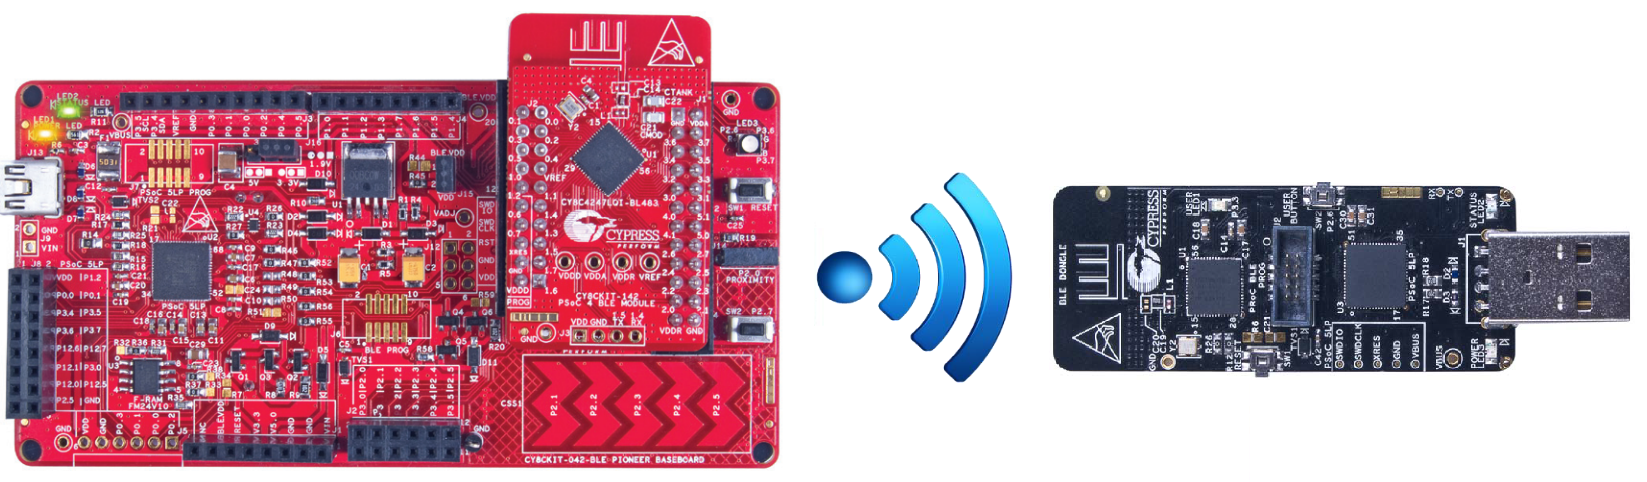
\includegraphics[width=1\textwidth]{figures/BLEToBLEdongle}
	\caption{Illustration af kommunikation mellem mikrokontroller og BLE dongle \citep{cypresspsoc2015, cypressguide2014}.}
	\label{fig:BLE_to_BLE_Dongle}
\end{figure}


Dette tillader således trådløs test, visualisering, og debugging af mikrokontrolleren. BLE-donglen forsynes via USB-porten på den givne computer med $5~V$ \citep{cypressguide2014}. Denne form for BLE-kommunikation anvendes for at kommunikere trådløst med en computer, således en visualisering er mulig. For at systemet senere skal kunne anvendes til ALS-patienter med gang, skal der tages højde for en maksimal forsinkelse, for at systemet kan følge almindelig gang. Gangfunktionen for ALS-patienter varierer alt efter, hvor mange funktioner der er nedsat, eksempelvis vil patienter med luftvejsproblemer gå langsommere. ALS-patienter har en gennemsnitlig gangfunktion på $1,02~m/s$ \citep{hausdorff2000}, hvorfor en forsinkelse på 100 ms vurderes at være acceptabel. Da systemet skal placeres på benet, vurderes det at en kommunikationsrækkevidde på $2~m$ er tilstrækkeligt.
\\

\textbf{Krav:}
\begin{itemize}
\item Mikrokontrolleren skal kommunikere trådløst med en computer
\item BLE-dongle skal forsynes via USB
\item Skal have en maksimal forsinkelse på 100 ms \fxnote{skal denne forsinkelse være større eller mindre?? - HUSK at ændre i brødteksten også!}
\item Skal have en kommunikationsrækkevidde på $2~m$
\end{itemize}



%%-----------------------Implementering-------------------------
\chapter{Implementering}

%%\section{Analog del}
\section{Analog del}
\begin{figure}[H]
\centering
\includegraphics[width=1\textwidth]{figures/implementering/Blokdiagram_analog.png}
\caption{Blokdiagrammets analoge del, der implementeres i det følgende afsnit.}
\label{fig:blokdiagram_analog1}
\end{figure}

\noindent
Til implementering af det analoge system, som er illustreret på \autoref{fig:blokdiagram_analog1}, bestemmes der ud fra de opstillede krav i afsnit \autoref{sec:analog_del_krav}, at der skal indgå EMG-signaler og accelerometre til signaloopsamling og behandling. For uden at leve op til de opstillede krav, var disse komponenter til rådighed. Til at forsyne EMG-signaler er der anvendt en spændingsforsyning, som ligeledes er en udleveret komponenten som opfylder kravene stillet i \autoref{sec:krav_spaending}.


%Til implementering af det analoge system, som er illustreret på \autoref{fig:blokdiagram_analog1}, bestemmes der ud fra de opstillede krav i \autoref{sec:analog_del_krav}, at der skal indgå en EMG-forstærker og accelerometre, der introduceres i \autoref{sec:EMG_krav} og \autoref{sec:acc_teori} i implementeringen af systemet. På baggrund af de overordnet krav til systemet er der valgt at anvende EMG og accelerometre, hvorudfra disse krav samt de opstillede krav har medvirket til tilvalg og fravalg af sensorer. Derudover har valget af EMG-forstærker og accelerometre til opsamling af EMG-signal og vinkler været afhængige af, hvilke komponenter der er til rådighed, som opfylder de opstillede krav. 





\subsection{Opsamling af accelerometer-signaler}
%Et accelerometer er en elektromekanisk enhed, som både kan måle statisk og dynamisk accerleration. Den statiske acceleration kan være tyngdekraften, hvor det er muligt at bestemme orienteringen af accelerometeret i forhold til jorden. De dynamiske kræfter såsom bevægelse, stød og vibrationer, gør det muligt at analysere accelerometeres bevægelse samt hastighed. 

I dette projekt anvendes der på baggrund af krav opstillet i \autoref{sec:acc_teori} to accelerometre ADXL335Z fra Analog Devices. Accelerometerne er en 3-aksialt sensor, som har et arbejdsområde på minimum $\pm~3~g$, og en spænding som output. Det analoge outputsignal er proportionalt med accelerationen \citep{analogdevices2009}. 

\noindent
Accelerometrene har en single-supply spændingsforsyning, som skal ligge mellem $1,8~-~3,6~V$.  Offsettet er afhængig af spændingen i spændingsforsyningen, da spændingen er $3,4~V$, bliver offsettet $1,7~V$, som er det halve af spændingsforsyningen. Båndbredden og støjen varierer for akserne. For x- og y-aksen ligger båndbredden mellem $0,5 - 1.600~Hz$ og støjen normalt på $150~\mu g/\sqrt{Hz}$ RMS. \fxnote{Den spektrale effekttæthed måles i $\mu g/$. Hvis dette divideres med kvadratroden af båndbredden af signalet $\sqrt{Hz}$, fås RMS af accelerationsstøjen ved en temperatur på $25^\circ$C} \citep{analogdevices2010}. %mens båndbredden for z-aksen ligger mellem $0,5 - 550~Hz$ og støjen normalt på $300~\mu g/\sqrt{Hz}$ RMS. 

Da accelerometrenes output er direkte proportienalt med dets input, afhænger sensitiviteten og offsettet af spændingen i spændingsforsyningen. Ved $3~V$ er sensitiviteten typisk $300~mV/g$ \citep{analogdevices2010}. 


\begin{figure}[H]
\centering
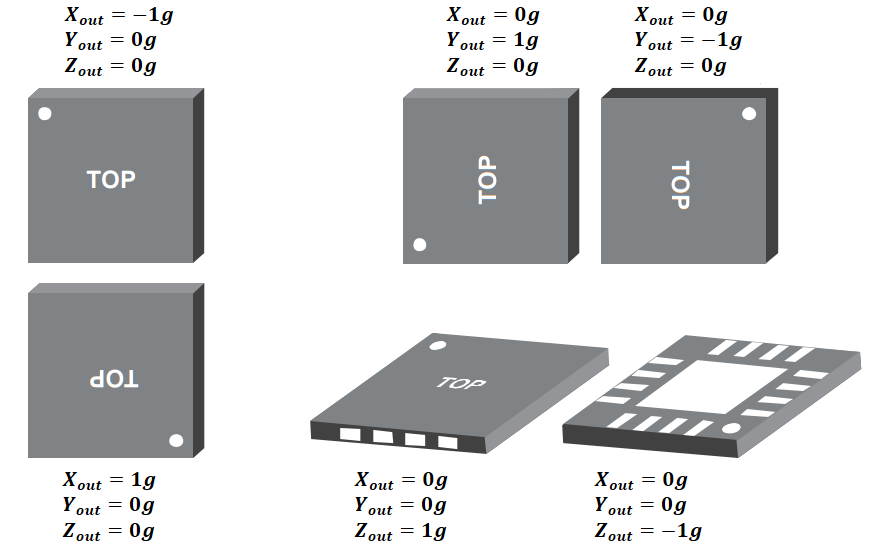
\includegraphics[width=0.85\textwidth]{figures/acc_paavirkning}
\caption{Påvirkning af accelerometeret i forskellige positioner. Til venstre måles accelerometeret lodret, til højre øverst vandret og til højre nederst i plan \citep{analogdevices2010}.}
\label{fig:acc}
\end{figure}

\noindent
Ved hældning af accelerometeret vil der ske en acceleration i forhold til tyngdekraften. Hvilken acceleration, der sker, er afhængigt af plan og hældningens retning. Dette fremgår af \autoref{fig:acc}. Herved vil der ske en ændring i outputspændingen ved en hældning på $0^{\circ}$. Hvis accelerometeret eksempelvis befinder sig i den øverste situation på \autoref{fig:acc}, påvirkes y-aksen med $-1~g$ \citep{clifford2005}. Denne sammenhæng og derved patientens hældning kan udtrykkes ved \autoref{equ:vinkler}, hvor $\phi$ er vinklen i forhold til udgangspunktet for den pågældende akse \citep{clifford2005}.

\begin{equation} \label{equ:vinkler}
	V_{out} = V_{offset} + sensitivitet \cdot \sin(\phi) \\
\end{equation}

\noindent

\subsection{Opsamling og behandling af EMG-signaler} \label{sec:EMG_imp}
For at opfylde de krav, der er opstillet i \autoref{sec:EMG_krav}, anvendes Muscle Sensor V3 fra Advancer Technologies, der fremover refereres til som 'EMG-forstærker'. 
Denne komponent måler en differens mellem de elektriske potentialer, der måles gennem elektroderne. 
EMG-forstærkeren består af en differensforstærker, et passivt højpasfilter, en helbølgeensretter, et aktivt lavpasfilter og en justerbar forstærker \citep{advancertech2013}. 

En illustration af, hvordan EMG-forstærkeren behandler et inputsignal fremgår af \autoref{fig:sinussignal}.
\begin{figure}[H]
\centering
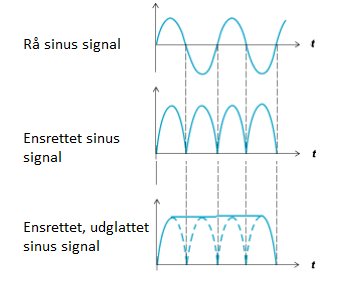
\includegraphics[width=0.6\textwidth]{figures/sinussignal.png}
\caption{Tre sinussignaler. Henholdsvis et råt, et ensrettet og et ensrettet samt udglattet sinussignal \citep{advancertech2013}.}
\label{fig:sinussignal}
\end{figure}

\noindent
På \autoref{fig:sinussignal} kan sinussignalet tolkes som et muskelsignal. 
Signalet passerer et passivt højpasfilter, der dæmper DC-støjen og dermed offsettet i signalet, hvilket medfører, at signalet centreres omkring 0. Dette fremgår af den øverste graf på \autoref{fig:sinussignal}. 
Centreringen er nødvendig for hensigtsmæssigt at ensrette signalet, da det ensrettes omkring tidsaksen. 
Denne ensretning er en helbølgeensretning, hvilket ses af den midterste graf på \autoref{fig:sinussignal}. 
Helbølgeensretning sker ved at invertere signalets negative værdier, således signalet kun har udslag i positiv retning. %Dette betyder at der ikke sker ændringer i det oprindelige signals energi. 
Herefter envelopefiltreres signalet, hvilket ses som det udglattede signal på nederste graf i \autoref{fig:sinussignal}. 

Envelopefilteret har til formål at stabilisere signalet, hvilket er implementeret i EMG-forstærkeren ved et lavpasfilter. 
Filtreret er beregnet til at have en knækfrekvens ($f_c$) på $1,94~Hz$ ud fra \autoref{eq:lavcutfre}. 
Denne  beregnes ud fra filtrerets modstande ($R$) og kondensatorer ($C$). 
Disse værdier er fundet i databladet for EMG-forstærkeren, hvor $C$ er aflæst til $1 \cdot 10^{-6}~F$ og $R$ til $80,6 \cdot 10^3~\Omega$ \citep{advancertech2013}. 

\begin{equation}\label{eq:lavcutfre}
f_c = \frac{1}{2 \pi C R} = \frac{1}{2 \pi \cdot 1 \cdot 10^{-6}~F \cdot 80,6 \cdot 10^3~\Omega} = 1,94~Hz
\end{equation}

\noindent
For at sikre, at EMG-forstærkerens forstærkning, ensretning og udglatning fungerer, kræver EMG-forstærkeren en spændingsforsyning på minimum $\pm 3~V$ og maksimalt $\pm 30~V$. Herudover er der mulighed for at justere modstanden fra $0,1~\Omega$ til $100~k\Omega$, hvilket giver et justerbart gain fra 0,002 til 20.700 gange, såfremt den forsynes med en spænding på $\pm 30~V$ \citep{advancertech2013}. 
\subsection{Spændingsforsyning}
For at opfylde kravene, der er specificeret i \autoref{sec:krav_spaending}, vælges det at benytte en færdigudviklet komponent, som bbenytter to $1,5~V$'s AA-batterier, der sidder i en spændingsregulator. Batteriernes kobling danner et split supply. De andre poler, som ikke anvendes til jordforbindelse, benyttes som systemets positive spændingsforsyning, ${V}_{cc}$ og negative spændingsforsyning, ${V}_{dd}$.

Spændingsregulatoren sørger for at give en konstant spænding på henholdsvis $3,4~V$ og $\pm 5,5~V$.\fxnote{Dette gøres ved, at spændingsregulatoren oplagrer spænding fra de to tilkoblede batterier i spoler, når switchfunktionen lukkes. Switchfunktionen åbnes, når spolerne er mættede og en spænding ledes videre i kredsløbet via en diode. Denne switchfunktion åbner og lukker skiftevis i kort tid, hvilket resulterer i, at en konstant spænding ledes til systemet hele tiden.} På sigt vil spændingsforsyningen ikke være i stand til at levere en jævn spænding grundet afladning af batterierne. I dette tilfælde vil spændingsregulatoren indikere dette ved at få en LED til at blinke, når der ikke leveres en konstant spænding. Yderligere vil LED'en stoppe med at lyse, når batterierne er helt afladede. 
Konfigurationen af spændingsforsyningen fremgår af \autoref{fig:spaendingsforsyning}, hvor terminalerne for $\pm 5,5~V$ fremgår som rød(V+) og blå(V-) og sort(Gnd), mens der på den modsatte side fremgår terminalerne for $3,4~V$ som brun(Vcc) og sort(Gnd). 

\begin{figure}[H]
\centering
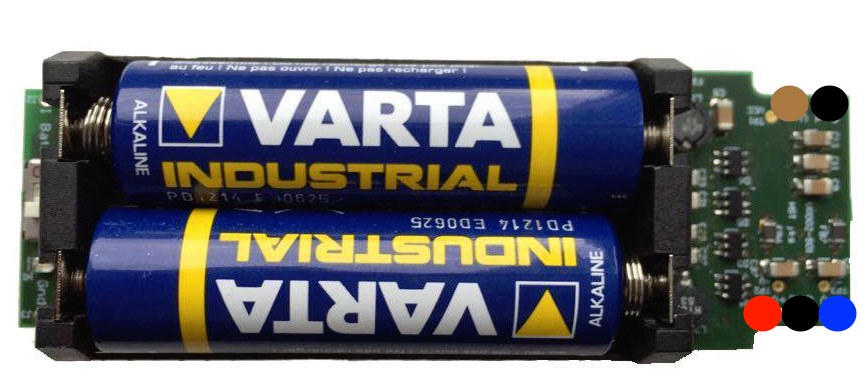
\includegraphics[width=0.6\textwidth]{figures/spaendingsforsyning}
\caption{Spændingsforsyning, der består af to $1,5~V$ batterier i et split supply. Den røde prik illustrerer V+, den blå V-, den sorte Gnd og den brune Vcc.}
\label{fig:spaendingsforsyning}
\end{figure}



%%\section{Digital del}
\section{Digital del}

\begin{figure}[H]
\centering
\includegraphics[width=1\textwidth]{figures/implementering/Blokdiagram_digital.png}
\caption{Blokdiagrammets digitale del, der vil blive implementeret i følgende afsnit.}
\label{fig:blokdiagram_digital1}
\end{figure}

Til implementering af det digitale system, som er illustreret på \autoref{fig:blokdiagram_digital1}, stilles der fra \autoref{sec:digital_del_krav} krav i forhold til implementeringen af ADC, filtrering og trådløs kommunikation. Da mikrokontrolleren er udleveret på dette semester er det et krav at anvende ADC'en på denne samt BLE-modulet, hvorfor A/D-konvertering og den trådløse kommunikation implementeres på denne. Derudover testes det, hvorvidt de forskellige filtre filtrere det uønskede signal fra. 




\subsection{Analog-to-Digital Converter}
Mikrokontrolleren indeholder en SAR ADC, som gør det muligt at konvertere det analoge signal til et digitalt. Der ønskes en konfigurering af 3 analoge kanaler, herunder Y-aksen på begge accelerometre samt EMG-forstærkeren. Opsætningen af ADC'en på mikrokontrolleren fremgår af \autoref{fig:ADC_teori}. Det ønskes at kunne læse signalerne hver for sig ved at måle single ended, hvorfor hvert input er tilkoblet $V_{ss}$. Da der ligeledes ønskes at anvende en 12 bit ADC på baggrund af kravet i \autoref{sec:ADC_teori}, indstilles denne til 12 bit. Da der anvendes single ended, svarer dette til at ADC'en anvender 11 bit, hvorfor den inddeles i $2^{11}$ svarende til 2048 niveauer. ADC'en har et arbejdsområde fra $0-5~V$. LSB'en for ADC'en kan beregnes ud fra \autoref{equ:LSB}, hvilket giver $2,44~mV$, hvis denne overskrides vil signalet gå i mætning \citep{ADC2014}. 


\begin{figure}[H]
\centering
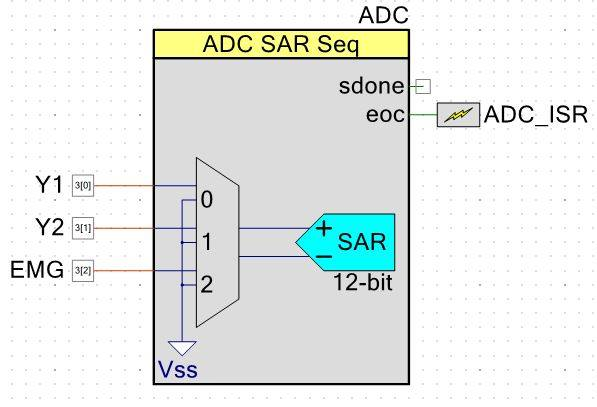
\includegraphics[width=0.5\textwidth]{figures/implementering/ADC_imp.jpg}
\caption{ADC'ens opsætning på mikrokontrolleren}
\label{fig:ADC_teori}
\end{figure}

I ADC'en er der indbygget en clock frekvens. Det er muligt at reducere konverteringstiden ved at øge ADC'ens clock frekvens. Når ADC'en skal starte på konverteringen, er det samplingstiden, der også måles som tiden i clock cycles. Der er forskellige parametre, der kan indstilles i PSoC, herunder opløsning, samplingsraten og clock frekvensen. Disse parametre bestemmer ADC'ens konverteringsrate. Konvertingstiden er den inverste af konverteringsraten. Clock frekvensen kan indstilles mellem $1000~MHz$ og $9000~MHz$.\citep{cypresspsoc42014} Da der ønskes at samples med 10 gange frekvensområdet for signalet, hvilket i følge  \autoref{sec:pilotforsoeg} er mellem 0,4 og $10~Hz$, vælges der at samples med $100~Hz$. Clockfrekvensen vælges til at have en hastighed på $1600~kHz$. Outputtet fra ADC'en er tilkoblet via eoc til ADC'ens Interrupt Service Routine (ISR), hvilket fremgår af \autoref{fig:ADC_teori}. Hvis der er sker et interrupt vil dette resultere i at de aktiverede kanaler er klar til at blive aflæst fra registrene, hvorved systemet igangsættes. \autoref{ADC2014} 



\subsection{Digital filtrering}
Det blev på baggrund af målinger i \autoref{sec:pilotforsoeg} og \autoref{sec:teori_filter} valgt at implementere et IIR-lavpasfiter og et moving average filter. 
Lavpasfiltreret har til formål at filtrere EMG-signalet, således det udglattes. Herudover skal lavpasfiltret følge det oprindelige signal. Moving average filtret har til formål at udglatte accelerometersignalerne med henblik på bedre repræsentation af vinkler. 
\subsubsection{IIR-lavpasfilter}
Det ønskede 2. ordens IIR-lavpasfilter er udarbejdet ud fra kravene opstillet i \autoref{sec:lavpas_krav}  og implementeres digitalt ved anvendelse af MATLAB og PSoC. 
Teorien hertil er beskrevet i \autoref{sec:teori_filter}. 
Ved implementering af dette filter benyttes MATLAB for således at beregne a- og b-koefficienterne for et Butterworth filter. 
For beregning af filtret anvendes \autoref{eq:iirfilt}. 

Koefficienterne fremgår af \autoref{tab:koeff_lav}. Dertil defineres a- og b-koefficienterne samt filterlængden i PSoC, hvorefter disse anvendes til programmering af lavpasfiltret. 

\begin{table}[H]
\centering
\begin{tabular}{|c|c|c|c|}
\hline
\textbf{a} & 1,0000 & -1,8890 & 0,0015 \\ \hline
\textbf{b} & 0,0015 & 0,0029  & 0,0015 \\ \hline
\end{tabular}
\caption{De udregnede a- og b-koefficienter for et Butterworth filter.}
\label{tab:koeff_lav}
\end{table}
\subsection{Implementering af et moving average filter}
Det ønskes at implementere et moving average filter ved anvendelse af MATLAB samt PSoC. Koefficienten, a, defineres til at have en værdi på 1, da denne er konstant ved FIR-filtre. Koefficienten, b, defineres ved at dividere a med filterlængden. Disse koefficienter findes i MATLAB og bliver overført til moving average filteret programmeret i PSoC. 

\subsection{Vinkelberegning}\label{sec:imp_vinkler}
I \autoref{sec:test_acc} fremgår det, at der er lineær sammenhæng mellem vinklerne over tid. Det er derfor muligt at udføre en lineær interpolation over dataen af målinger fra accelerometrene i forskellige vinkler. På denne måde er det muligt at bestemme, hvilken som helst vinkel for en tilsvarende spænding. Da målingerne af linearitet, målt i \autoref{sec:test_acc}, er foretaget med Ni USB-6009 stemmer spændingerne ikke overens, når det samples på mikrokontrolleren. Derfor udføres der en ny måling af linearitet med mikrokontrolleren, hvor spændingen i de forskellige vinkler er målt. Efterfølgende er der aflæst et offset, som er trukket fra, for at centrere signalet omkring 0. Offsettet for accelerometeret placeret på låret er aflæst til $-1003~V$ og accelerometeret placeret på skinnebenet til $-972~V$. De målte spændinger, hvor signalet er offsetjusteret fremgår af \autoref{tab:vinkelinterval_psoc}. .

%\begin{comment}
%\begin{table}[H]
%	\centering
%	\begin{tabular}{|l|l|l|}
%				%& \textit{Accelerometer placeret på låret} &				
%	\textbf{Interval} & \textbf{Målt spænding} & \textbf{Målt spænding} 	\\ \hline	
%    \textbf{0-10} 			& $0~V$							& $-186~V$   \\ \hline
%    \textbf{10-30} 			& $-31~V$						& $-185~V$	\\ \hline
%    \textbf{30-50} 			& $-67~V$						& $-168~V$	\\ \hline
%    \textbf{50-70} 			& $-126~V$						& $-126~V$	\\ \hline
%    \textbf{70-80} 			& $-168~V$						& $-67~V$	\\ \hline
%    \textbf{80-90} 			& $-185~V$						& $-31~V$	\\ \hline
%    				%& \textit{Accelerometer placeret på skinnebenet} &		
%    	\textbf{Interval} & \textbf{Målt spænding} & \textbf{Målt spænding} 		\\ \hline	
%    \textbf{0-10}			& $0~V$ 							& $-179~V$	    \\ \hline
%    \textbf{10-30}			& $-16~V$						& $-176~V$	 	\\ \hline
%    \textbf{30-50}			& $-52~V$						& $-153~V$		\\ \hline
%    \textbf{50-70}			& $-111~V$						& $-111~V$		\\ \hline
%    \textbf{70-80}			& $-153~V$						& $-52~V$	 	\\ \hline
%     \textbf{80-90}			& $-176~V$						& $-16~V$	 	\\ \hline
%	\end{tabular}
%	\caption{Spændingen målt i vinklerne fra 0 til 90$^{\circ}$ for accelerometrene placeret på både låret og skinnebenet. Den første spænding svarer til start intervallet og den sidste til slutningen afintervallet.}
%	\label{tab:vinkelinterval_psoc}
%\end{table}
%\end{comment}


\begin{table}[]
\centering
\begin{tabular}{|l|c|c|}
         & \textit{Accelerometer placeret på låret}                           & \multicolumn{1}{l}{}                      \\ \hline
Interval & Målt spænding {[}V{]}                                              & \multicolumn{1}{l}{Målt spænding {[}V{]}} \\ \hline
0 - 10   & 0                                                                  & - 31                                      \\ \hline
10 - 30  & - 31                                                               & - 67                                      \\ \hline
30 - 50  & - 67                                                               & - 126                                     \\ \hline
50 - 70  & - 126                                                              & - 168                                     \\ \hline
70 - 80  & - 168                                                              & - 185                                     \\
\hline
80 - 90  & -185                                                               & - 186                                     \\
\hline
         & \multicolumn{1}{l}{\textit{Accelerometer placeret på skinnebenet}} & \multicolumn{1}{l}{}                      \\ \hline
Interval & Målt spænding {[}V{]}                                              & \multicolumn{1}{l}{Målt spænding {[}V{]}} \\ \hline
0 - 10   & 0                                                                  & - 16                                      \\
\hline
10 - 30  & - 16                                                               & - 52                                      \\
\hline
30 - 50  & - 52                                                               & - 111                                     \\
\hline
50 - 70  & - 111                                                              & - 153                                     \\
\hline
70 - 80  & - 153                                                              & - 176                                     \\
\hline
80 - 90  & - 176                                                              & - 179    \\ \hline 
\end{tabular}
\caption{Spændingen målt i vinklerne fra 0 til 90$^{\circ}$ for accelerometrene placeret på både låret og skinnebenet. Den første spænding svarer til start intervallet og den sidste til slutningen afintervallet.}
\label{tab:vinkelinterval_psoc}        
\end{table}

Spændingen er målt for vinklerne fra 0 til 90$^{\circ}$ for accelerometrene placeret på både låret og skinnebenet. Den første målte spænding er for startværdien i intervallet og den sidste spænding er slutværdien i intervallet.

Ud fra de målte værdier i de forskellige intervaller, er der opstillet en funktion indeholdt ifelse-løkker, hvorved det er muligt at vurdere, hvilket interval en given spænding befinder sig i. I hver enkelt løkke anvendes lineær interpolation, som har til opgave at finde en vinkel, der er svarende til en spænding som ligger mellem intervallet og returnerer denne. 

Når der er udført lineær interpolation over dataen skal de målte data fra låret samt skinnebenet ligges sammen for at få den samlede vinkel af, hvor langt personen har bevæget sig, og derved befinder sig i squat-øvelsen. Resultaterne er optaget på mikrokontrolleren og visualiseres i MATLAB, hvilket fremgår af \autoref{fig:acc_imp}.
 

\begin{figure}[H]
\centering
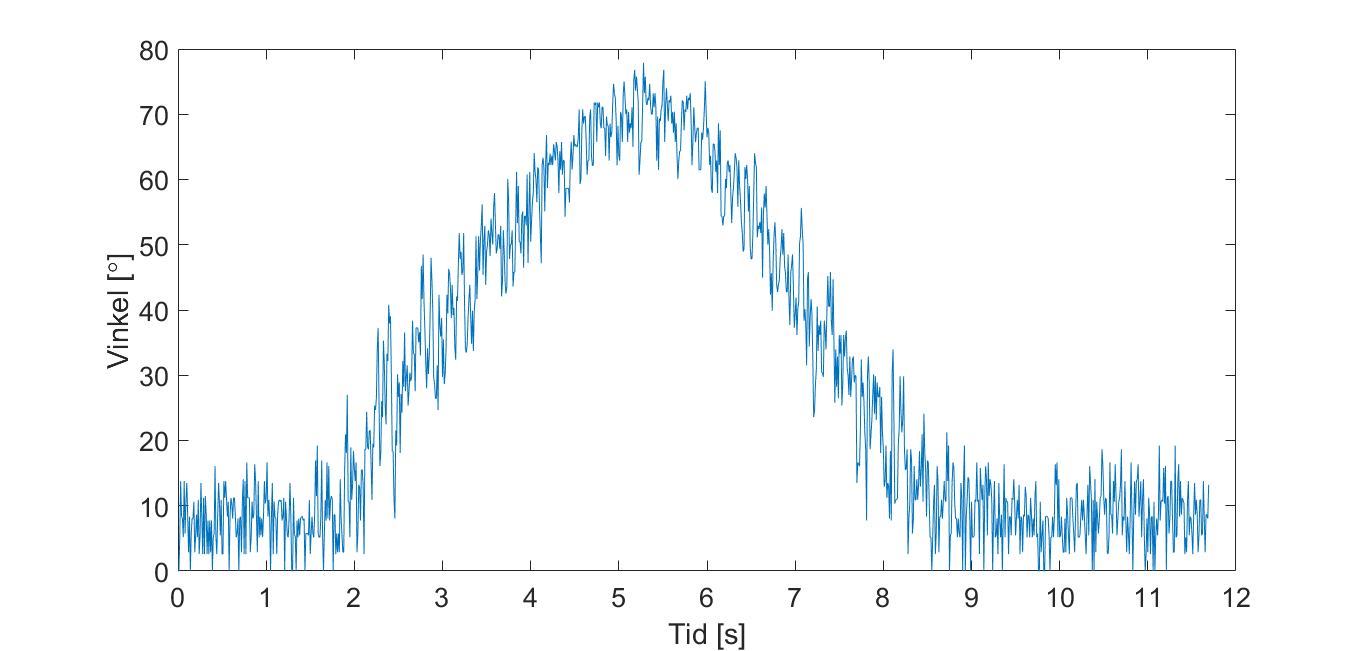
\includegraphics[width=0.8\textwidth]{figures/Pilotforsoeg/accvinkel}
\caption{Samlet vinkler af accelerometrene under udførelse af squat-øvelsen}
\label{fig:acc_imp}
\end{figure}



 
\subsection{EMG-algoritme}
For at opfylde kravene fra \autoref{sec:krav_emg_algo} skal hældningen af EMG-signalet findes. Dette kan gøres ved differentiering, hvorved det vil være muligt at finde hældningen af én sample ved differentialkvotienten. Det vælges at implementere en mere simpel metode til at tilnærmelsesvist at finde hældningen ved \autoref{eq:haeldning}, hvorved tangentens hældning findes.s

\begin{equation}
f'(x)\approx\dfrac{\Delta y(x)}{\Delta x}
\label{eq:haeldning}
\end{equation}

\noindent
I \autoref{eq:haeldning} er $\Delta x$ tiden mellem to samples, og $\Delta y(x)$ den målte spænding fra rectus femoris til tiden $x$. 

Hvis $f'(x)>1$ skal der gives et output på $10$, som signalerer til prototypen, at knæleddet skal flekse. Hvis derimod $f'(x)<1$ skal der gives et output på $-10$, som signalerer til prototypen, at knæleddet skal ekstendere. Derudover skal funktion give et output på $0$, hvis knæets vinkel ikke befinder sig i intervallet $90$-$180^{\circ}$
\section{Trådløs kommunikation}
Den trådløse kommunikation er designet til direkte kommunikation mellem mikrokontrolleren og NXT'en til at styre exoskelettet. Herudover skal der etableres en trådløs kommunikation til en computer til debugging, test af mikrokontrolleren samt datavisualisering.   

\noindent
Til implementeringen af den trådløse kommunikation tages der ikke udgangspunkt i det oprindelige design. Dette er som følge af opsætningen af bluetooth kommunikationen i mikrokontrolleren, er fremkommet til at være mere kompliceret end først antaget. Dette omfatter, at der kræves en forståelse for diverse bluetooth programmeringsbiblioteker samt relaterede funktioner til at programmere buletooth kommunikation. For at implementere dette, vil den krævede tid således blive for lang og usikker i forhold til den endelige funktionalitet.
Dertil vælges det at implementere et mere simpelt og anvendeligt alternativ, bestående af to PSoC 4 M-Series Prototyping Kit board, der ses af \autoref{fig:PSoC_4200}

\begin{figure}[H]
	\centering
	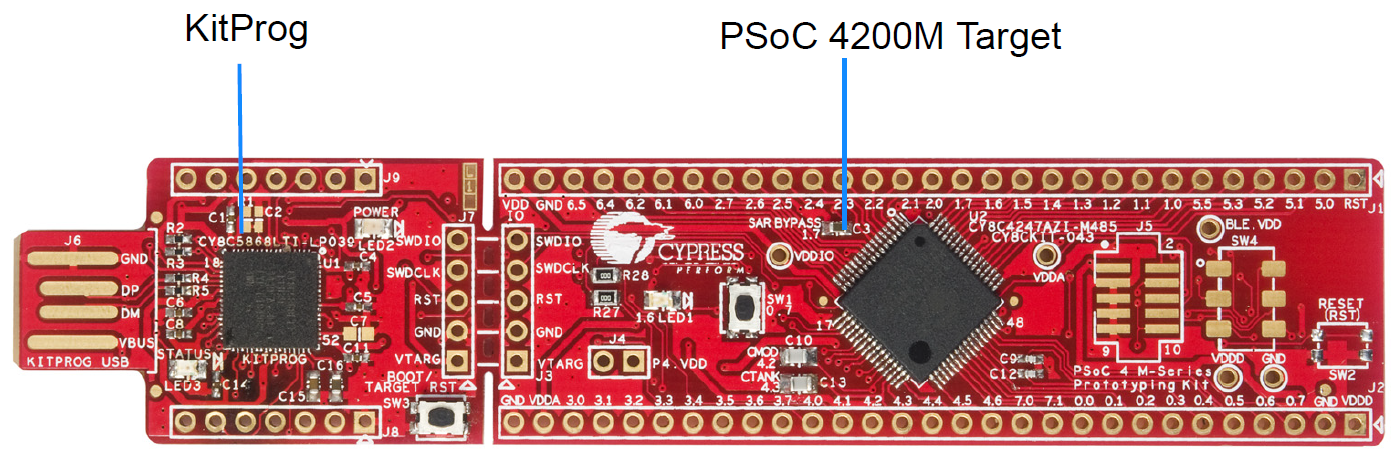
\includegraphics[width=0.8\textwidth]{figures/PSoC_4200_opdelt}
	\caption{CY8CKIT-043 PSoC 4 M-Series Prototyping Kit\citep{cypress42015}.}
	\label{fig:PSoC_4200}
\end{figure}

Dette board består af en KitProg og en PSoC 4200M enhed. KitProgen anvendes til at debugge og programmere koden. PSoc 4200M er processoren, hvorpå koden eksekveres. Yderligere er boardet udstyret med et EZ-BLE modul, der tillader trådløs kommunikation ved brug af bluetooth low energy. 
Den ene PSoC 4200M tilkobles mikrokontrollern via UART forbindelse og den anden tilsluttes computeren via USB og erstatter BLE donglen fra det oprindelige design. En illustration af, hvordan kommunikationen transmiteres i det implementerede system fremgår af \autoref{fig:Traadloes_Komm_Imp}.

\begin{figure}[H]
	\centering
	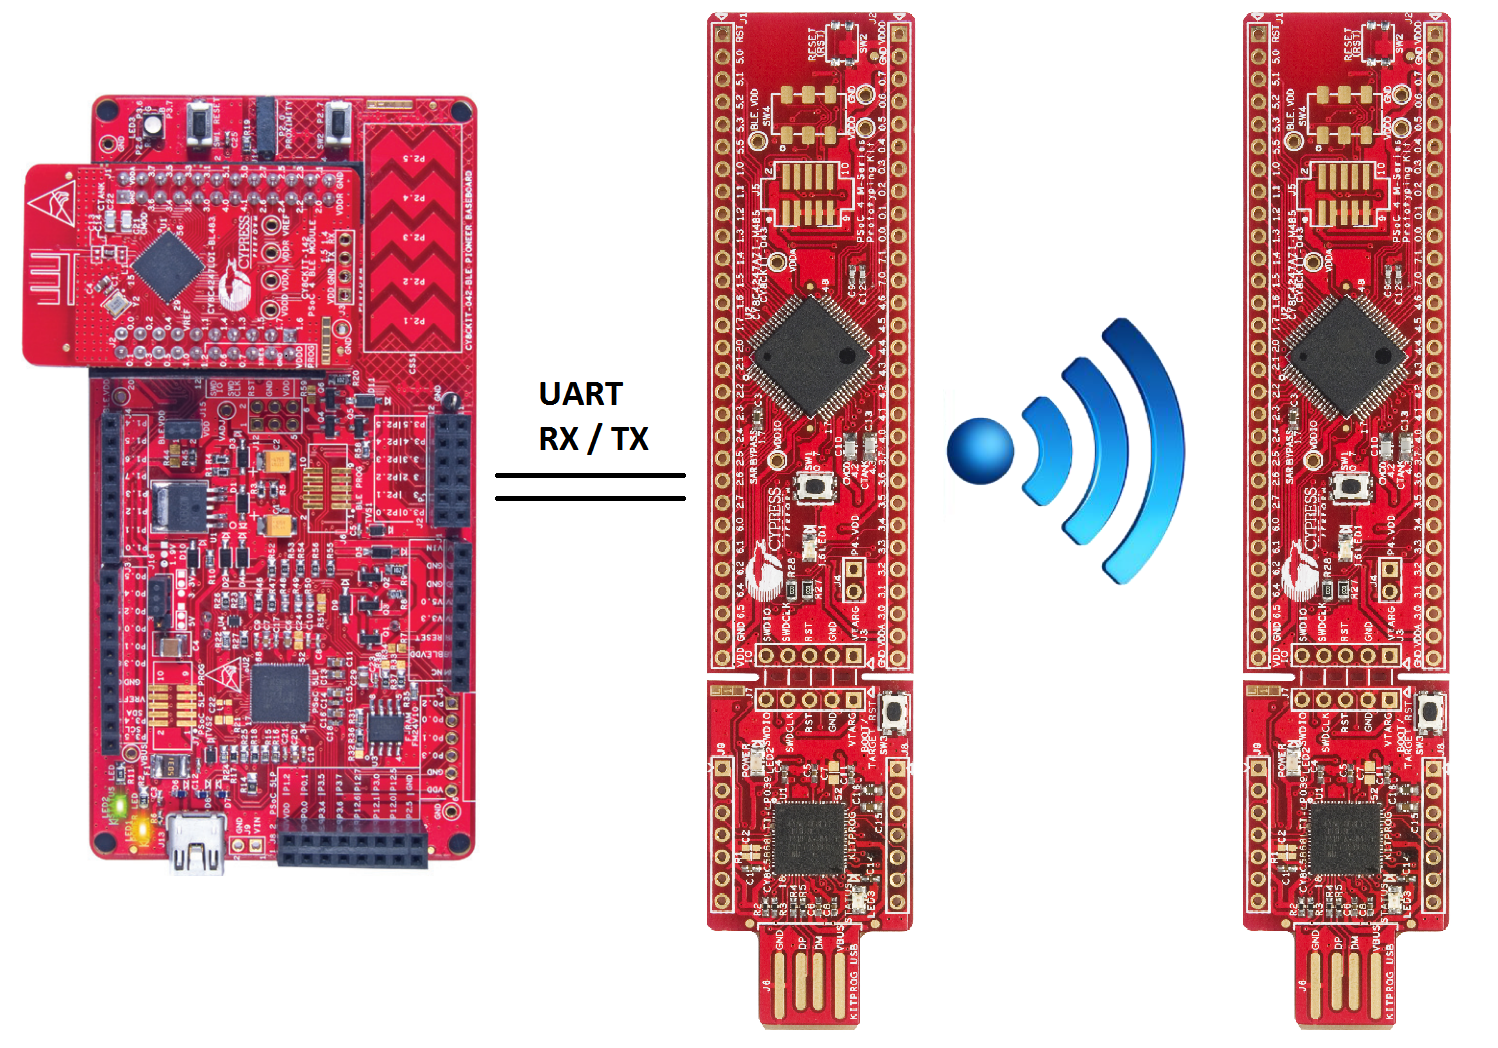
\includegraphics[width=0.8\textwidth]{figures/Traadloes_Komm_Imp}
	\caption{Illustration af kommunikation mellem mikrokontroller og computer. Der ses UART forbindelse til venstre, hvor der er anvendes RX (receive) og TX (transmit). Til højre ses indikeringen af tråløskommunikation ved brug af BLE.} 
	\label{fig:Traadloes_Komm_Imp}
\end{figure}

Opsætningen, der fremgår af \autoref{fig:Traadloes_Komm_Imp} er mere anvendeligt, da der tages udgangspunkt i kodeeksempler til PSoC 4200M, hvorpå den trådløse kommunikation i forvejen er programmeret. Dertil er det ikke nødvendigt at opsætte BLE kommunikation, men alene, hvordan data'en skal videregives. 
Begge PSoC 4200M enheder programmeres til at 'echo' information, der modtages via BLE eller UART og transmitere det videre. Dertil vil data modtaget fra mikrokontrolleren blive videregivet til den ene PSoC4200M enhed, hvorpå data transmiteres trådløst til den anden PSoC4200M enhed. Derfra sendes data via UART til computeren. 
For at de to PSoC4200M enheder kan kommunikere med hinanden, progammeres EZ-BLE modulerne til at være henholdsvis central og peripheral. Dette betegner en rolle, der gives de to PSoC4200M enheder, hvor central oftest er enheden med mest processorkraft og hukommelse og den peripheral enhed oftest er en mindre og ressourcebegrænset enhed \citep{townsend2014}. I dette system er mikrokontrolleren anset som en primær komponent, hvortil den tilsluttede PSoC 4200M enhed defineres som central. Ved aktiv data transmission vil en indikering i form af en blå led på den centrale PSoC 4200M lyse.
%\subsection{Low power mode}

Der findes forskellige grader af low power mode. Herunder en sleep mode, deep-sleep mode, hibernate mode og stop mode. Systemet anvender sleep mode, hvor alle periphals udover CPU'en er tilgængelig. Systemet befinder sig i sleep mode hele tiden og kører dermed ingen instruktioner. Den venter i stedet på, at der forekommer et interrupt. Et hvert interrupt kan anvendes til at vække systemet fra sleep mode, herefter vil systemet gå ud af sin sleep mode, når der er udløst et interrupt. 

Det kan være fordelagtigt at anvende sleep mode, når eksempelvis ADC'en eller digital kommunikation, hvor andre peripherals skal forblive aktive, men uden CPU'ens aktivitet er nødvendig. På denne måde vil det være muligt at reducere strømforbruget mellem AD-konvertinger samt transaktioner under den digitale kommunikation.\citep{cypresspsoc420152}

\subsection{Flowdiagram}
I dette afsnit fremgår implementeringen af systemets blokke fra \autoref{sec:blokdiagram}. Disse flowdiagrammer er anvendt for at visualisere opbygningen samt sammenhængen mellem blokkene. Flowdiagrammene er opdelt og består af et overordnet, som beskriver hele processen og et initialiserende samt et, der viser EMG-algoritmen. Udover den visualiserende del vil det blive uddybet, hvilke funktioner de enkelte figurer indeholder. Anvendelsen af de forskellige figurer i flowdiagrammerne er beskrevet i \autoref{sec:flowhaandtering}.

\subsubsection{Overordnet flowdiagram}
Det analoge signal, som optages af de implemterende sensorer skal konverteres fra analogt til digitalt, hvorved det efterfølgende kan implementeres i softwaren. Det overordnede flowdiagram fremgår af \autoref{fig:overordnet_flow}. For at implementering af softwaren vil foreløbe skal der ske et interrupt ved at trykke på PSoC'ens user button, som får en grøn LED til at lyse og derefter igangsætter de efterfølgende funktioner. Dette igangsætter et timer interrupt, der tæller inden for XX interval. Herefter sker der en intialisering af systemet.
\begin{figure}[H]
\centering
\includegraphics[width=0.8\textwidth]{figures/implementering/overordnet_flow.png}
\caption{Overordnet flowdigram som viser opbyggelsen af systemet}
\label{fig:overordnet_flow}
\end{figure}



\subsubsection{Initialiserende flowdiagram}
I intialiseringsprocessen, der fremgår af \autoref{fig:initialiserende_flow} sker opsætningen af ADC'en. Efter modtagelsen af det analoge input sker en A/D-konvertering, hvor det analoge signal digitaliseres. For at kunne behandle dataen og kommunikere trådløst igangsættes et setup, hvor BLE tilkobes og signalet offsetjusteres. Efter setup skal det vurderes, hvorvidt inputtet befinder sig inden for en spænding svarende til 0 til 90 graders vinkel, hvis dette er tilfældet, vil signalet starte EMG-algoritmen, hvilket fremgår af det overordnede flowdiagram, der fremgår af \autoref{fig:overordnet_flow}. 
\begin{figure}[H]
\centering
\includegraphics[width=0.8\textwidth]{figures/implementering/initialiserende_flow.png}
\caption{Initialiserende flowdigram som viser opbyggelsen af den intialiserende del af systemet}
\label{fig:initialiserende_flow}
\end{figure}

\subsubsection{EMG-algoritme}
EMG-algoritmen fremgår af \autoref{fig:Emg_algo}. Hvis inputtet fra accelerometret svarer til en spænding mellem 0 og 90 grader vurderes det, hvorvidt muskelaktiviteten er faldende eller stigende. Én sample sammenlignes med den efterfølgende sample for at vurdere, om muskelaktiviteten er stigende eller faldende. Hvis muskelaktiviteten er stigende, vil vinklen blive større, og herved slutter EMG-algoritmen og sender et input til prototypen med BLE, hvorved en fleksion af knæleddet påbegyndes. Hvis muskelaktiviteten er faldende, vil vinklen blive mindre, hvilket ligeledes slutter EMG-algoritmen og sender et input videre til BLE, hvorved en ektension af knæleddet påbegyndes. 
\begin{figure}[H]
\centering
\includegraphics[width=1.0\textwidth]{figures/implementering/EMG_algo.png}
\caption{EMG-algoritmen viser opbyggelsen af EMG-algortimens del af systemet.}
\label{fig:Emg_algo}
\end{figure}


\subsection{Samlet system}
Under implementering af det samlede system er det nødvendigt at ændre flere parametre for at kunne opfylde de overordnet krav, beskrevet i  \autoref{sec:overordnet_krav}. Dette omfatter ændring af forsyningen af spænding til de enkelte komponenter, hvilket forårsager at spændingen for de udregnede vinkler er ændret.

\subsubsection{Forsyning af spænding}
Da systemet skal være batteridrevet, skal alle komponenter kobles til et batteri. Dette implementeres ved at mikrokontrollen, gum sticken og EMG-forstærkeren får spænding fra spændingensregulatoreren, der leverer en spænding på $5,5~V$ til disse komponenter. Mikrokontrolleren er koblet til de to accelerometre og forsyner disse med en spænding på $3,3~V$. Opsætningen af dette er illustreret på \autoref{fig:samlet_spaending_imp}. 

\begin{figure}[H]
\centering
\includegraphics[width=0.5\textwidth]{figures/samlet_spaending}
\caption{Illustration af koblingen af spænding til de enkelte komponenter.}
\label{fig:samlet_spaending_imp}
\end{figure}

\subsubsection{Beregning af vinkler}
Da spændingen accelerometrene modtager ændres fra $3,4$ til $3,3~V$, bliver offsettet for disse ligeledes ændret. Dette gør sig gældende da disse afhænger af hinanden, som  beskrevet i \autoref{sec:acc_imp}. Offsettet for accelerometeret placeret på låret er $-1,5904~V$, og for accelerometeret placeret på skinnebenet er $-1,5598~V$. Dette medvirker til, at de udregnede vinkler for intervallet $90-180^{\circ}$ ændres. De nye vinkler fremgår af \autoref{tab:samlet_vinkel_imp}. 

\begin{table}[H]
\centering
\begin{tabular}{|c|c|c|}
\hline
\multicolumn{1}{|l|}{\textbf{Vinkel {[}$^{\circ}${]}}} & \textbf{\begin{tabular}[c]{@{}c@{}}Digital output fra acclerometer \\ placeret på låret\end{tabular}} & \textbf{\begin{tabular}[c]{@{}c@{}}Digital output fra accelerometer \\ placeret på skinnebenet\end{tabular}} \\ \hline
\textbf{0}                                                      & -195                                                                               & -170                                                                                      \\ \hline
\textbf{10}                                                     & -191                                                                             & -164                                                                                     \\ \hline
\textbf{30}                                                     & -165                                                                             & -142                                                                                    \\ \hline
\textbf{50}                                                     & -122                                                                            & -101                                                                                   \\ \hline
\textbf{70}                                                     & -60
& -42                                                                                   \\ \hline
\textbf{80}                                                     & -25	
& -4                                                                                   \\ \hline
\textbf{90}                                                     & -0                                                                            & -0                                                                                   \\ \hline
\end{tabular}
\caption{Digitalt output fra accelerometer placeret på låret og skinnebenet svarende til en given vinkel.}
\label{tab:samlet_vinkel_imp}
\end{table}



%%-----------------------Test-------------------------%%
\chapter{Test}
%%\section{Analog del}
\section{Analog del}
\begin{figure}[H]
\centering
\includegraphics[width=1\textwidth]{figures/implementering/Blokdiagram_analog.png}
\caption{Blokdiagrammets analoge del}
\label{fig:blokdiagram_analog1}
\end{figure}


For at kunne teste om de enkelte komponenter i den analoge del, som fremgår af \autoref{fig:blokdiagram_analog1}, opfylder kravene stillet i \autoref{sec:analog_del_krav} testes delene hver for sig. Testen af sensorerne omhandler opsamling af signal og hvordan det er muligt at gøre dette. Der testes her for om der opsamles det forventede signal. I forhold til spændingsforsyningen testes der for om den leverer en jævn spændingen, hvilket kan få betydning for hele kredsløbet, hvis dette krav ikke bliver opfyldt.
\subsection{Opsamling og behandling af EMG-signaler}

EMG-forstærkeren testes for at vurdere, hvorvidt der kan opsamles muskelaktivitet fra rectus femoris. Overfladeelektroderne placeres ud fra SENIAM's anvisning om elektrodeplacering, jf. \autoref{sec:pilotforsoeg}. En squat-øvelse udføres, hvorved muskelsignaler A/D-konverters ved brug af mikrokontrolleren og visualiseres i MATLAB. Denne øvelse er beskrevet i \autoref{sec:knaeled_squat}. Muskelsignalet under udførslen af squat-øvelsen fremgår af \autoref{fig:raat_emg}. 

\begin{figure}[H]
\centering
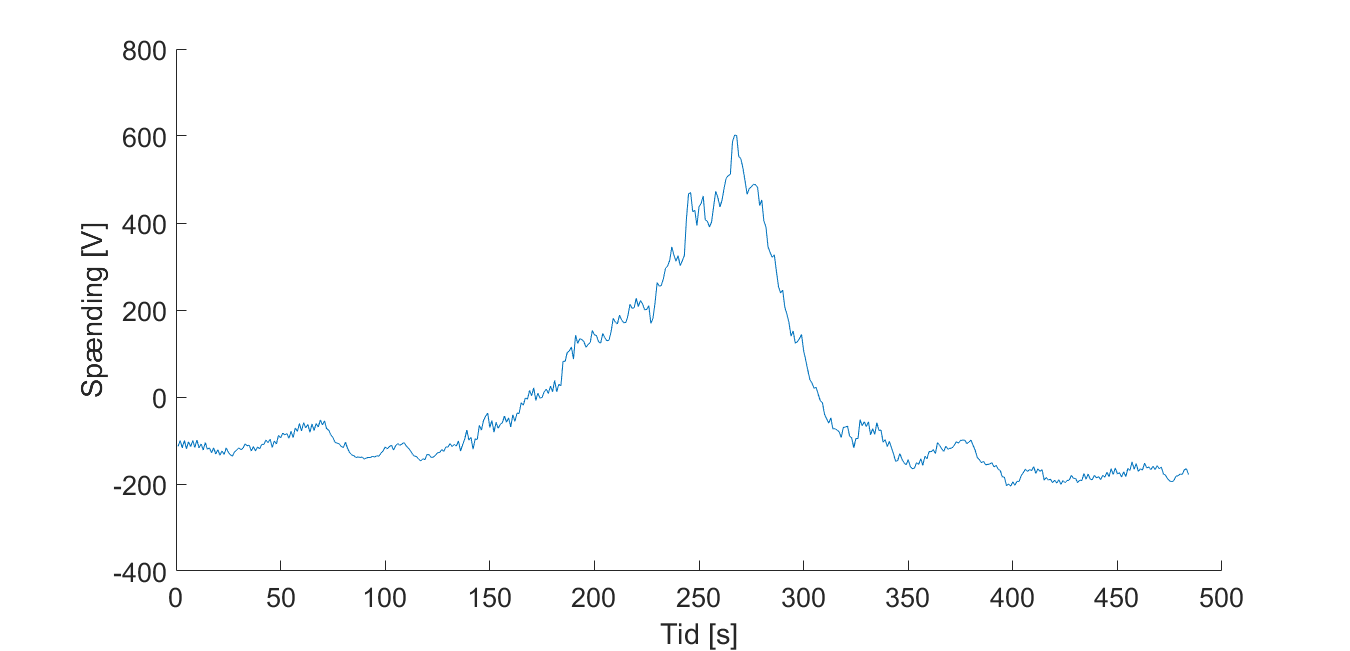
\includegraphics[width=1\textwidth]{figures/raat_EMG_test}
\caption{Et samplede EMG-signal fra rectus femoris under udførsel af en squat-øvelse.}
\label{fig:raat_emg}
\end{figure}

\noindent
Ud fra \autoref{fig:raat_emg} ses den opsamlede muskelaktivitet fra rectus femoris. For således at undersøge, hvorvidt muskelsignalerne ligger i frekvensområdet mellem $10-500~Hz$ er en frekvensanalyse foretaget. Grundet EMG-forstærkerens virkemåde forventes det at frekvensområdet er mere lavfrekvent, da det envelopefilteres. Dette fremgår ligeledes af frekvensanalyse foretaget i \autoref{sec:pilotforsoeg}, hvor det blev vurderet til at ligge  mellem $0,4-10~Hz$. Hertil fortages yderligere en frekvensanalyse af signalet der ses i  \autoref{fig:raat_emg} og fremgår af \autoref{fig:fft_raat_emg}.

\begin{figure}[H]
\centering
\includegraphics[width=1\textwidth]{figures/fft_raat_EMG}
\caption{Frekvensanalyse af samplet EMG-signal under en squat-øvelse, hvor Y-aksen er en semilogaritmisk skala}
\label{fig:fft_raat_emg}
\end{figure}

\noindent
Frekvensanalysen sammenlignes med analysen foretaget i \autoref{sec:pilotforsoeg}, hvortil der ikke ses nogen yderligere forskel. Dertil er det eneste bevis for at EMG-forstærkeren opsamler frekvenser passende til kravet, at der reelt forekommer udslag i målingen i det muskelen kontraherer.    
 
EMG-forstærkeren forsynes med en spænding på $\pm 5,4~V$, hvilket er testet i \autoref{test_spaendingsforsyning} og derved overholder kravet om minimum $\pm 5~V$.
På EMG-forstærkeren findes et justerbart gain, således forstærkningen kan tilpasses den enkelte bruger af systemet. Ud fra dette og \autoref{fig:raat_emg} vurderes det, at EMG-forstærkeren opfylder de opstillede krav i \autoref{sec:EMG_krav}.

\vspace{3mm}
\textbf{Opsummering af krav:}
\begin{itemize}
\item[\text{\sffamily \checkmark}] Skal opsamle muskelsignal
\item[\text{\sffamily \checkmark}] Skal være anvendeligt med overflade elektroder
\item[\text{\sffamily $\div$}] Skal opsamle muskelsignaler i frekvensområdet mellem $10$ og $500~Hz$
\begin{itemize}
\item[\text{\sffamily \checkmark}] Grundet EMG-forstærkerens virkemåder bliver outputsignalet lavfrekvent, hvortil frekvensområdet er aflæst til at være mellem $0,4-10~Hz$
\end{itemize}
\item[\text{\sffamily \checkmark}] Skal forsynes med en spænding på minimum $\pm5~V$
\item[\text{\sffamily \checkmark}] Skal have et justerbart gain, der kan tilpasses den enkelte bruger af systemet
\end{itemize}


\subsection{Opsamling af accelerometer-signaler}

Accelerometrene testes for at vurdere, hvorvidt de opstillede krav i \autoref{sec:acc_teori} opfyldes. 
Det fremgår af databladet, at accelerometrene er triaksiale.  
Ud fra målinger foretaget i \autoref{sec:test_acc} ses en lineær tendens med en afvigelse på maksimalt $3~\%$, hvilket derfor lever op til kravet for lineariteten. Da det ikke er muligt at teste om accelerometrene har accelerationer i $\pm2~g$, tages der udgangspunkt i databladet. I databladet beskrives det, at accelerometrene har et lineært arbejdsområde på $\pm 3~g$.
Accelerometrene kan ud fra databladet forsynes med en DC-forsyning fra $1,8-3,6~V$ \citep{analogdevices2009}. Kravet hertil er, at accelerometrene skal forsynes med en minimum spænding på $3~V$. Det er derfor testet, hvorvidt mikrokontrolleren forsyner accelerometrene med denne spænding. Testen er udført ved brug af et multimeter, hvortil der måles en spænding på $3,2~V$. Test af mikrokontrolleren er udført i \autoref{sec:samlet_system}, hvorved kravet om en minimum spænding på $3~V$ er opfyldt.

\vspace{3mm}
\textbf{Opsummering af krav:}
\begin{itemize}
\item[\text{\sffamily \checkmark}] Skal måle på minimum Y-aksen
\item[\text{\sffamily \checkmark}] Skal have en linearitet med en afvigelse på $5\%$
\item[\text{\sffamily \checkmark}] Skal måle accelerationer i $\pm2~g$
\item[\text{\sffamily \checkmark}] Skal forsynes med en spænding på minimum $3~V$
\end{itemize}


\subsection{Spændingsforsyning} \label{test_spaendingsforsyning}
Det forventes, at spændingsforsyningen leverer en konstant spænding til EMG-forstærkeren på minimum $\pm 5~V$, hvilket fremgår af \autoref{EMG_krav}. For at undersøge, om spændingsforsyningen opfylder de opstillede krav i \ref{sec:krav_spaending}, testes spændingsforsyningen med et multimeter, hvor outputspændingen måles. %Ét kabel tilsluttes $V_{cc}$, og ét andet tilsuttes ground. 
Ud fra dette er den positive spænding målt til $5,574~V$ og den negative spænding til $-5,341~V$, hvilket giver en peak-to-peak-amplitude på $10,815~V$. Årsagen til at dette afviger fra de oplyste værdier i \autoref{sec:krav_spaending}, relateres til at det ikke er en ideel komponent. 

%
%Under testen, blev der ikke set udslag på multimeteret, hvorved spændingsforsyningen overholder kravet om at skulle kunne levere en konstant spænding. Dette betyder at spændingsforsyningen kan levere en spænding, som er passede for at forsyne EMG-forstærkeren.
Derudover testets der for om spændingsregulatoren signalerer et signal via en LED, hvis den ikke leverer en konstant spændingen. Under forsøget blev der anvendt nye batterier og afladede batterier. Ved at anvende nye batteriet blev det målt af spændingsregulatoren leverede en spænding på $\pm5,4~V$, hvortil LED'en lyste konstant. Ved de afladede batterier blev spænding målt til  $0,0985~mV$, hvortil LED'en ikke lyste. Dokumentation for denne test fremgår af \autoref{fig:spaendingsforsyning_LED}.


\begin{figure}[H]
\centering
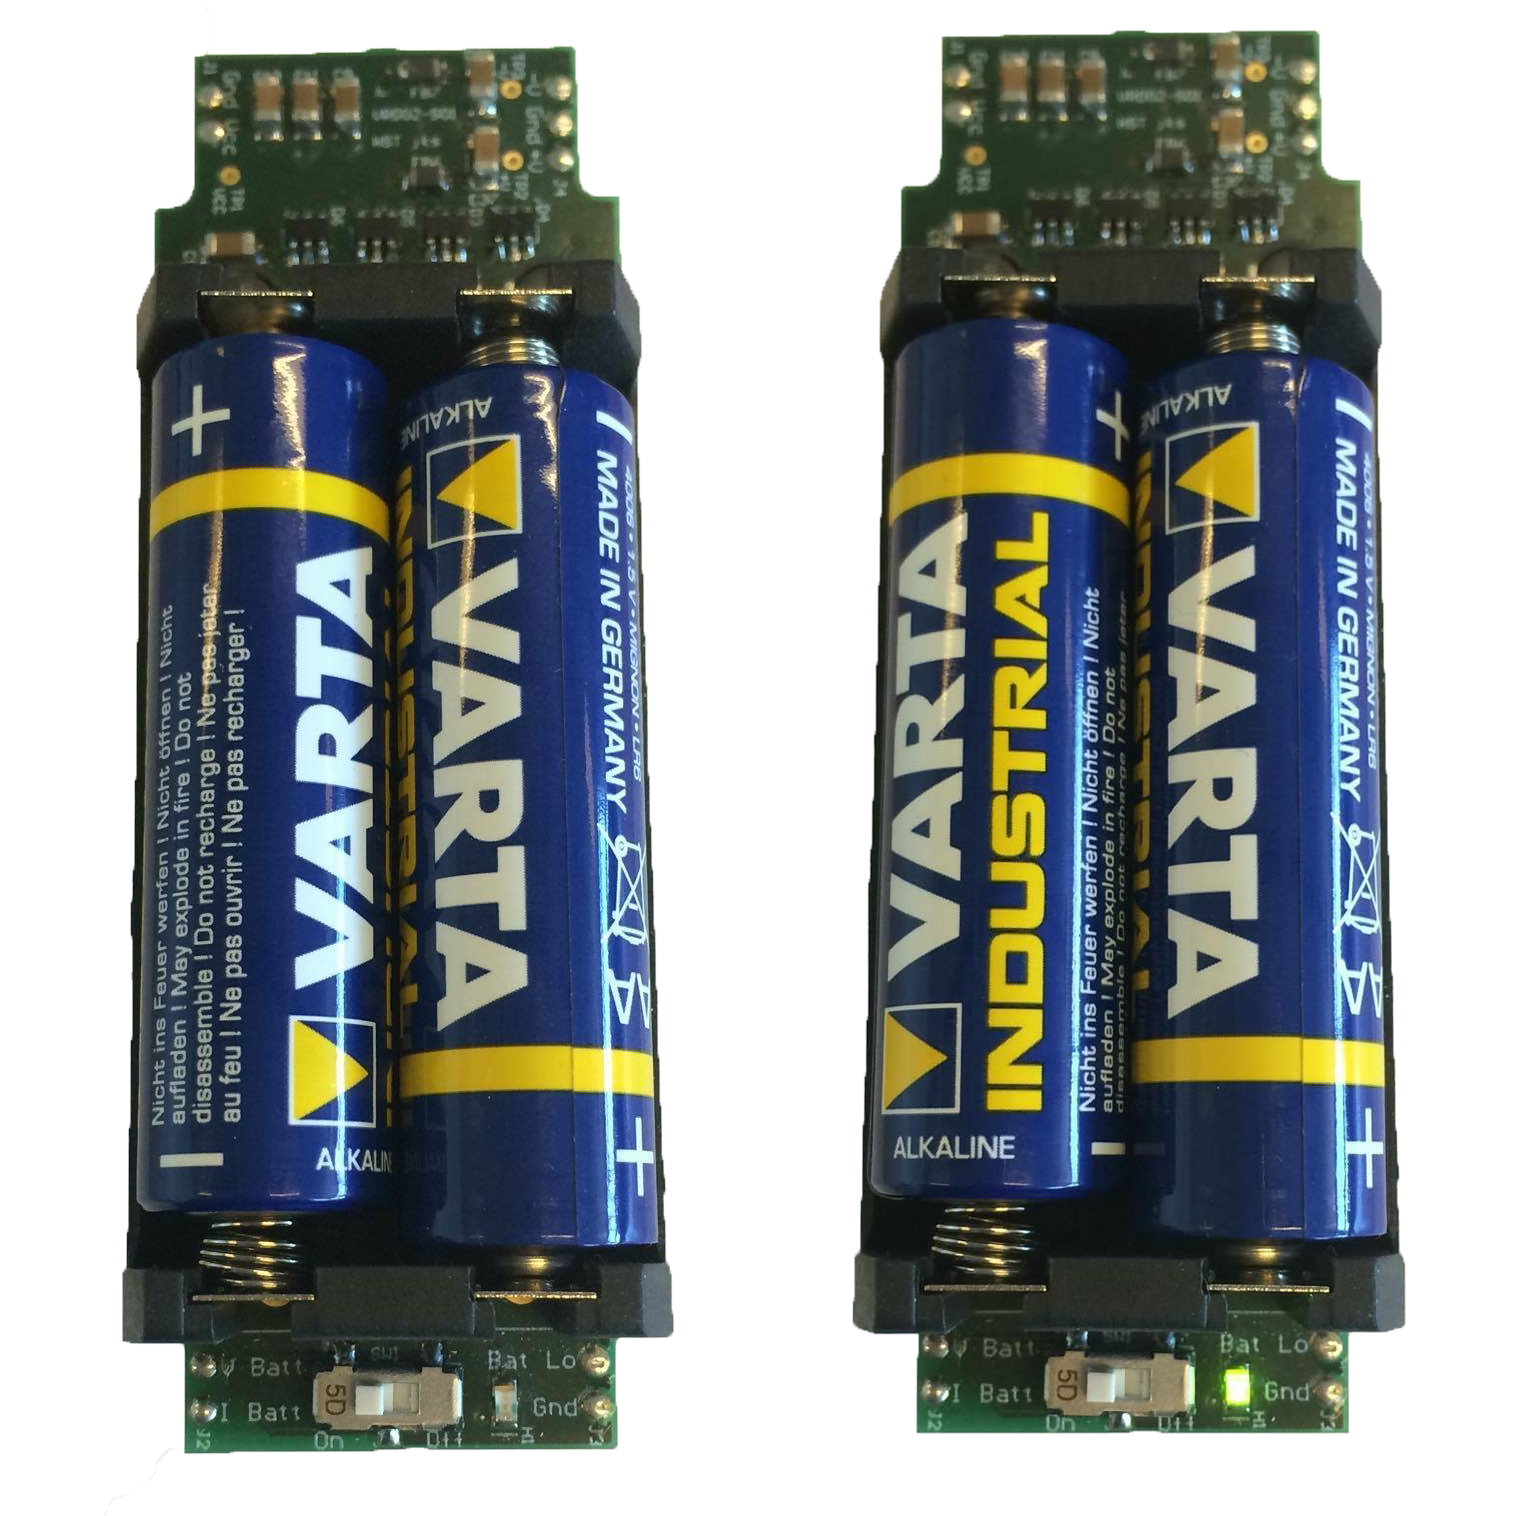
\includegraphics[width=0.6\textwidth]{figures/bat_test}
\caption{Billedet til højre viser spændingsregulatorens når den leverer en spænding på $5,4~V$, hvorved en grøn LED lyser for indikere dette. Billedet til venstre viser spændingsregulatoren når den ikke leverer en passende spænding, hvormed LED'en er slukket.}
\label{fig:spaendingsforsyning_LED}
\end{figure}

\vspace{3mm}
\textbf{Opsummering af krav:}
\begin{itemize} 
\item[\text{\sffamily \checkmark}] Skal kunne forsyne aktive komponenter i den analoge del af kredsløbet
\item[\text{\sffamily \checkmark}] Skal kunne levere en konstant spænding
\item[\text{\sffamily \checkmark}] Skal kunne give et signal, hvis der ikke leveres en konstant spænding
\end{itemize}

 

%%\section{Digital del}
\section{Digital del}
\begin{figure}[H]
\centering
\includegraphics[width=1\textwidth]{figures/implementering/Blokdiagram_digital.png}
\caption{Blokdiagrammets digitale del}
\label{fig:blokdiagram_digital1}
\end{figure}

For at undersøge om systemet opfylder kravene i \autoref{sec:digital_del_krav}, skal den digitale del af systemet som vist på \autoref{fig:blokdiagram_digital1} testes. Dette gøres ved at teste de enkelte blokke hver for sig og vurdere om de opfylder de stillede krav. Udover de viste blokke i blokdiagrammet testes der for vinkelberegning og EMG-algoritme, som anvendes for at systemet kan udføre en squat-øvelse på baggrund af disse funktioner.   
\subsection{Analog-to-Digital Converter}

For at teste, hvorvidt ADC'em kan sample tre inputs, foretages en test, hvorpå 3 kanaler opsættes. Dette fremgår af \autoref{fig:treinput}.

\begin{figure}[H]
\centering
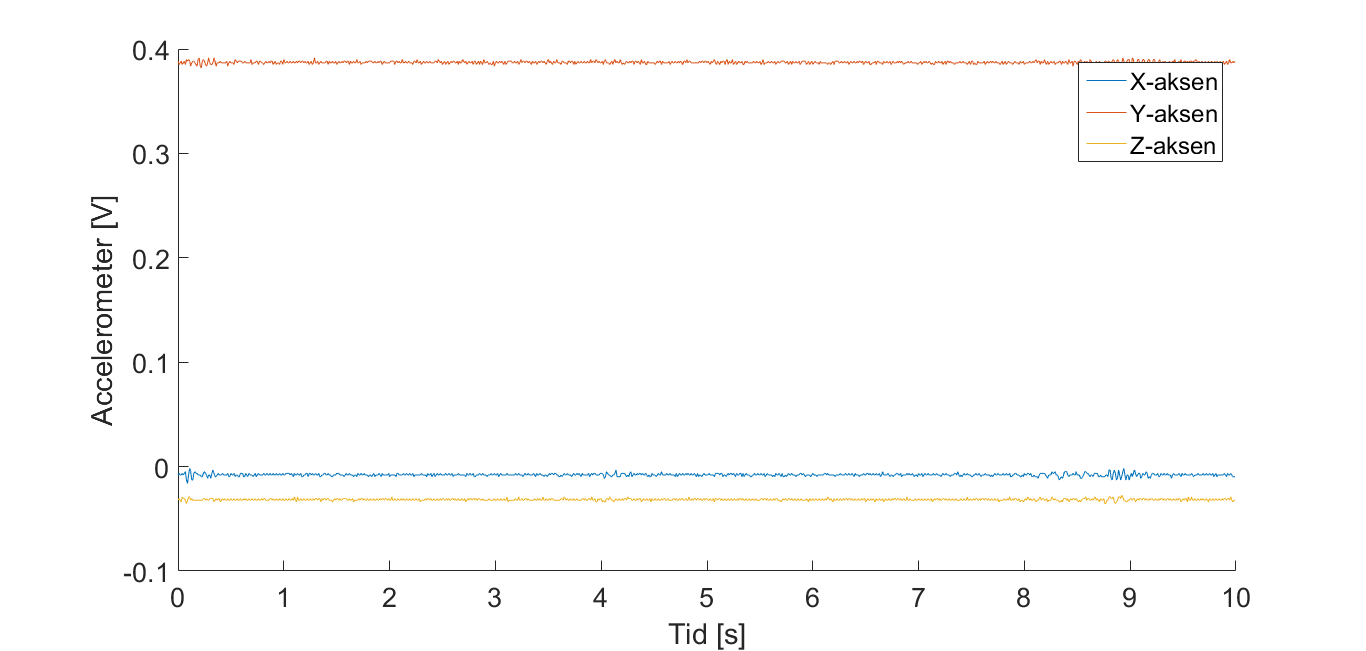
\includegraphics[width=1\textwidth]{figures/treinput}
\caption{Tre input samlpet samt visualiseret i MATLAB. Input-signalet er samplet fra acceleromterets tre akser.}
\label{fig:treinput}
\end{figure}

\noindent
Det ses af \autoref{fig:treinput}, at ADC'en herved kan sample 3 inputs fra et accelerometer. Kanalerne kan herved ændres til et ønsket inputsignal eksempelvis et muskelsignal. 

På baggrund af \autoref{sec:ADC_imp} er der valgt at anvende en ADC med et arbejdsområde på $2^{11}$, hvilket vurderes at være acceptabel og ikke forringer det ønskede signal under konverteringen. Dette ses ligeledes af \autoref{fig:treinput}.

Det fremgår \autoref{sec:pilotforsoeg} at frekvensområdet for muskelaktivitet befinder sig relativt lavfrekvent mellem $0,4-10~Hz$. Derved anses en samplingfrekvens på $100~Hz$ tilstrækkeligt. 

Derudover fremgår det af \autoref{fig:treinput}, at signalet ikke overstiger ADC'ens arbejdsområde under store udsving af accelerometersignalet. Hertil forventes det, at signalet ikke overstiger arbejdsområdet ved det endelige system, da bevægelsen herunder er kontrolleret og med mindre udsving.

ADC'ens samplingsfrekvens testes for at undersøge om den indstillede og reelle samplerate er identisk. Til denne test defineres en variable, som tæller op for hver gang, at der er konverteret data fra ADC'en. Hvis en konvertering mislykkes vil den givende sample ikke registreres. De registrerede værdier videresendes via USB-forbindelse mellem computer og mikrokontroller, hvorefter dataen aflæses i MATLAB. 
Testen foretages i 30 minutter, hvorved konverteringen samt tid startes på samme tid. De registrede data aflæses, hvorved en samplingsfrekvens udregnes af \autoref{eq:ADC_test}. Antallet af konverteringer målt under testen er $177066~samples$ over en periode af $1800,16~s$.

\begin{equation}\label{eq:ADC_test}
Fs = \frac{177066~samples}{1800,16~s}
\end{equation}

\noindent
Der forventes en samplingsfrekvens på $100~Hz$. Den reelle frekvens er udregnet til $98,36~Hz$ ud fra \autoref{eq:ADC_test}. Dette giver en afvigelse på $1,64\%$. Afvigelsen kan relateres til, at tiden og konverteringen ikke har været startet og stoppet på præcis samme tid. Dette resulterer i, at der ikke er en direkte relation mellem køretiden for ADC'en og tiden. Yderligere tillader indstillingerne for ADC'en, at der kan ændres i konverteringstiden for de enkelte kanaler, men samtidig oplyse, at der bevares en aktuel samplingsfrekvens på $100~Hz$. Dette antages ligeledes at have en indflydelse på samplingsfrekvensen, selvom den oplyses som værende $100~Hz$. 

Tiltrods for afvigelsen godkendes ADC'en indstillinger. Dette relateres til, at lavfrekvente signaler samples, og at størrelsen på afvigelsen ikke har betydning for repræsentationen af signalerne. 
Med henblik på den endelige anvendelse i form af et exoskellet, vil systemet ligeledes skulle følge kroppens naturlige bevægelse. Hertil fremhæves, at exoskelletet ikke skal tilpasse en ny position 100 gange i sekundet, da det ville være uhensigtsmæssigt.


\vspace{3mm}
\textbf{Krav:}
\begin{itemize}
\item[\text{\sffamily \checkmark}] Skal sample minimum tre inputs 
\item[\text{\sffamily \checkmark}] Skal have en opløsning, der ikke forringer signalet
\item[\text{\sffamily \checkmark}] Skal have en samplingsfrekvens omkring 10 gange større end den højeste signalfrekvens
\item[\text{\sffamily \checkmark}] Skal undgå, at signalet ikke overstiger ADC'ens arbejdsområde
\item[\text{\sffamily \checkmark}] Samplingsfrekvensen skal have en maksimal afvigelse på $2~\%$
\end{itemize}


\subsection{Digital filtrering}
De implementerede filtre på PSoC, herunder lavpasfilter og moving average, testes for at undersøge om de opfylder de opstillede krav i \autoref{sec:lavpas_krav}. 
Det vurderes, hvorvidt det filtrede signal følger det ufiltrede signal. 
\subsection{Test af lavpasfilter}
For at teste om lavpasfilteret fungerer efter kravene stillet i \autoref{sec:lavpas_krav} visualiseres forskellen mellem det ufiltrede signal og det filtrede signal. Signalerne der sendes ind er fra det optagede signal fra pilotforsøget \autoref{sec:pilotforsoeg}. Disse sendes til mikrokontrollen via UART-forbindelse, hvorved der modtages den retunerede værdi. De sendte og returnerede værdier er visualiseret i MATLAB og fremgår af \autoref{fig:lavpas_imp}

\begin{figure}[H]
\centering
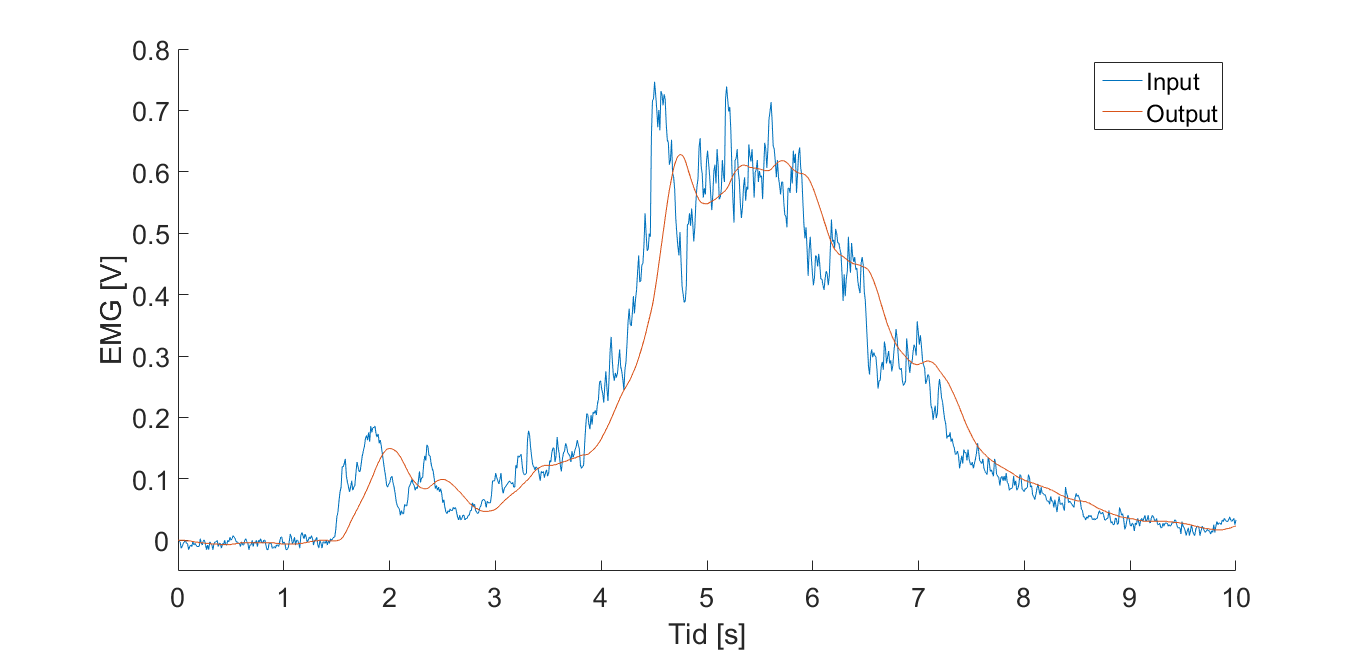
\includegraphics[width=0.8\textwidth]{figures/EMG_test}
\caption{Lavpasfilter lavet på mikrokontrolleren visualiseret i MATLAB}
\label{fig:lavpas_imp}
\end{figure}

På baggrund af disse resultater fremgår at de ønskede krav om maksimal fladhed samt undgå ripples ved brug af Butterworth lavpasfilter er overholdt. 
Deruodver fremgår det at inputsignalet følger det ufiltrede signal dog med et delay. Til måling af behandlingstiden af dette, programmeres en timer funktion i mikrokontrolleren, der retunerer behandlingstiden til MATLAB. Ud fra dette ses et delay på 39 sekunder og 56 milisekunder.


For at vurdere om filteret dæmper i forhold til de opstillede krav, udføres en sweep-test af frekvenser fra $0-15~Hz$ med en funktionsgenerator. Dette frekvensområde er valgt på baggrund af målinger fra \autoref{sec:pilotforsoeg}, hvor det fremgår at signalet ligger mellem $0,4-10Hz$.  Da funktionsgeneratoren ikke kan indstilles til en frekvens på $0~Hz$ indstilles denne til $1 \mu~Hz$. Amplituden sættes til $1~Vpp$. Resultatet af denne test fremgår af \autoref{fig:lavpas_sweep}. 


\begin{figure}[H]
\centering
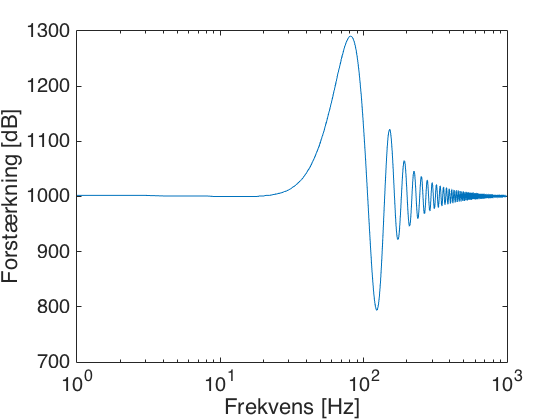
\includegraphics[width=0.8\textwidth]{figures/bodeplot_lavpas}
\caption{Bodeplot fra sweep-test af et filterede signal sinus signal med en frekvens på $1\mu~Hz$ til $15~Hz$.}
\label{fig:lavps_sweep}
\end{figure}

På baggrund af disse resultater fremgår at de ønskede krav om en knækfrevens på ...


\subsubsection{Moving average filter}
Moving average filteret testes for at undersøge, hvorvidt de opstillede krav overholdes, samt undersøge om designet er korrekt implementeret. Måden, hvorpå dette testes er ved anvendelse af data fra pilotforsøget, da dette giver kontrolleret testforhold. 
En computer med MATLAB benyttes til at sende en givende måling til mikrokontrolleren, hvorpå det digitale filter er implementeret. Mikrokontrolleren returnerer løbende den filtrerede værdi, der visualiseres i MATLAB. Ud fra dette ses om filteteret virker hensigtsmæssigt. 
Resultatet af denne test fremgår af \autoref{fig:mavg_test}. 

\begin{figure}[H]
	\centering
	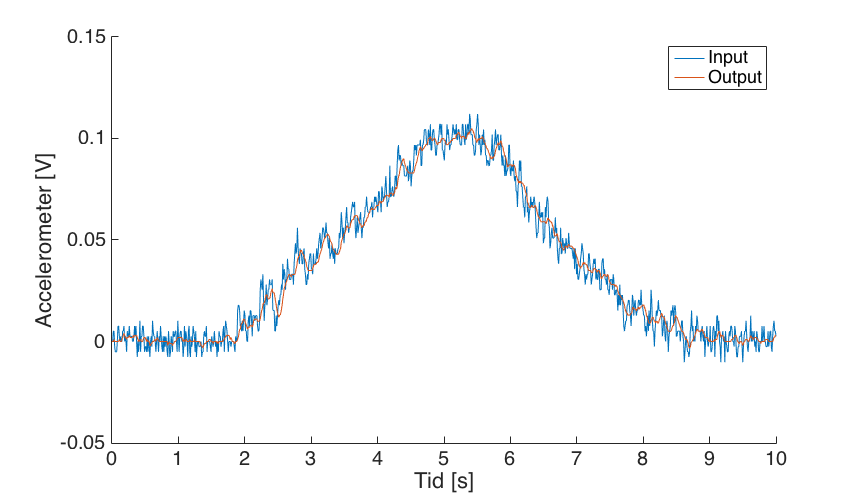
\includegraphics[width=1\textwidth]{figures/accelerometer_filter}
	\caption{Den blå graf illustrerer et ufiltreret signal fra accelerometer og den røde graf illustrerer et filtreret signal fra accelerometer, visualiseret i MATLAB}
	\label{fig:mavg_test}
\end{figure}

\noindent
Da filteret kræver 10 samples for at retunere den første værdi testes det, hvorvidt dette stemmer overens med det forventede forsinkelse på $100~ms$. Dertil er endnu en test foretaget, hvor et signal genereres i MATLAB. Dette signal sendes igen ind i mikrokontrolleren, hvortil et moving average filter pålægges. Herved er forsinkelsen beregnet. En visualisering af denne test ses af \autoref{fig:forsinkelse}

\begin{figure}[H]
	\centering
	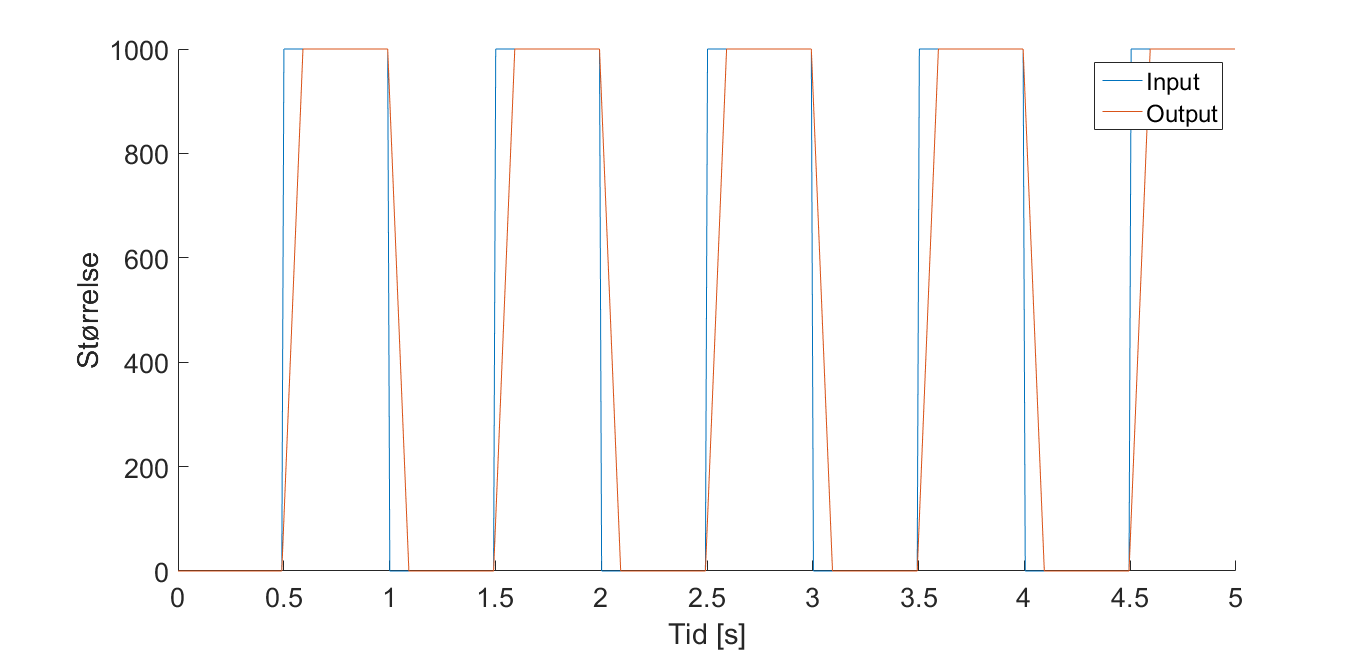
\includegraphics[width=1\textwidth]{figures/forsinkelse}
	\caption{Den blå graf illustrerer et ufiltreret signal, genereret i MATLAB og den røde graf illustrerer det filtreret signal, visualiseret i MATLAB}
	\label{fig:forsinkelse}
\end{figure}

\noindent
Resultatet fra denne test viser en forsinkelse af moving averge filteret på $0,09$ senkundt, hvilket er lavere end den forventede forsinkelse på $0,1$ sekundt og derfor accepteres. 

Yderligere foretages en test af forsinkelsen, der forekommer i det filteret eksekveres. Til denne test er en debug pin blevet defineret, hvor denne pin sættes som høj før funktionskaldet og lav efter funktionskaldet. Et oscilloscope tilsluttes debug pinen, således det kan måles, hvor længe debug pinen er høj. Resultatet fra testen er en forsinkelse på $320~\mu s$ for data at passere filteret. Dette betragtes som værende ikke af signifikant betydning.    
Ud fra ovenstående resultater vurderes det, at det filterede signal opfylder kravene for \autoref{sec:mavg_krav}. 


\vspace{3mm}
\textbf{Opsummering af krav:}
\begin{itemize}
\item[\text{\sffamily \checkmark}] Skal muliggøre en repræsentation af spændinger 
\item[\text{\sffamily \checkmark}] Skal have en filterlængde på $10$ samples
\item[\text{\sffamily \checkmark}] Skal have en maksimal forsinkelse på $100~ms$
\end{itemize}
\subsection{Accelerometeralgoritme}

For at teste, om omregningen fra spændingen til vinkler fungerer i praksis, bevæges vinkeltesteren, der er vist på \autoref{fig:vinkeltest}, fra $180^{\circ}$ til $70^{\circ}$. 
Figur \ref{fig:spaending_vinkel_test} illustrerer dette i MATLAB, hvor vinklen er illustreret på den venstre Y-akse, og hvor accelerometrenes spænding er illustreret på den højre Y-akse.

\begin{figure}[H]
\centering
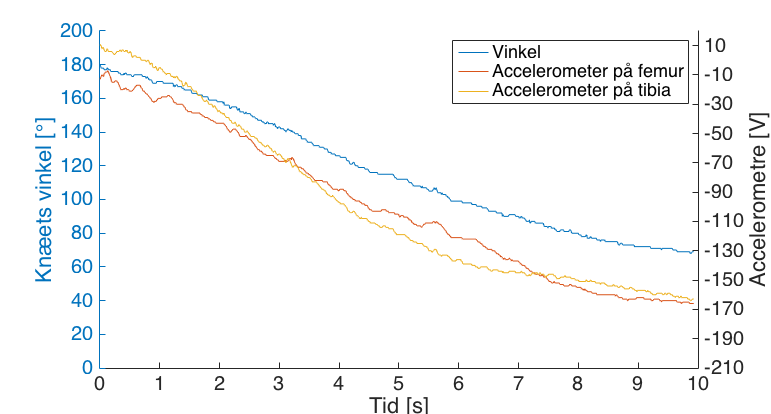
\includegraphics[width=1\textwidth]{figures/spaending_vinkel_test}
\caption{Test af vinkelberegning. Vinklen, som er den blå graf, er svarende til den samlede vinkel mellem de to accelerometre, hvor værdierne er illustreret på Y-aksen til venstre i grader. Spændingen målt for de to accelerometre måles i forhold til Y-aksen til højre og er vist ved en rød og gul graf.}
\label{fig:spaending_vinkel_test}
\end{figure}

\noindent
Det ses på \autoref{fig:spaending_vinkel_test}, at der er en sammenhæng mellem spænding fra accelerometrene og den samlede vinkel over knæleddet. 
Der tages udgangspunkt i \autoref{tab:vinkelinterval_psoc} for omregningen, hvoraf spændingen for hvert accelerometer omregnes til grader. 
Disse lægges sammen for at udregne den samlede vinkel. 
Derudover illustrerer figuren, at vinklerne virker inden for det forventede arbejdsområde på $90$-$180^{\circ}$, dertil kan vinklen over knæet ligeledes bestemmes under $90^{\circ}$. 
På figuren aflæses, at systemet registrerer en vinkel på $90^{\circ}$, når  accelerometeret på femur giver en spænding på $-0,2191~V$ og accelerometeret på tibia giver en spænding på $-0,2336~V$. 

For at teste vinkelberegningen sammenlignes de målte spændinger for accelerometrene, der er illustreret på \autoref{fig:spaending_vinkel_test}, og de konverterede digitale outputværdier i \autoref{sec:imp_vinkler}, der er omregnet til en tilsvarende spænding. 
De omregnede spændinger fra accelerometrene er lagt sammen for at få den samlede spænding, der opnås ved en tilsvarende vinkel. 
Resultaterne heraf fremgår på \autoref{tab:vinkel_test_afvigelse}.

\begin{table}[H]
\centering
\begin{tabular}{|c|c|c|c|}
\hline
\textbf{Vinkel {[}{$^{\circ}$}{]}} & \textbf{Implementeret spænding {[}V{]}} & \textbf{Målt spænding {[}V{]}} & \textbf{Afvigelse {[}\%{]}} \\ \hline
\textbf{180}                    & 0                         & -0,00323                       & 0,3                      \\ \hline
\textbf{160}                    & -0,1136                   & -0,11118                       & 2,1                       \\ \hline
\textbf{140}                    & -0,2150                   & -0,2240                        & 4,2                   \\ \hline
\textbf{100}                    & -0,4044                   & -0,4109                        & 1,6                    \\ \hline
\textbf{80}                     & -0,5447                   & -0,4906                        & 3,4                    \\ \hline
\end{tabular}
\caption{Udregnede afvigelser mellem de implementerede og målte spændinger inddelt efter vinkler på henholdsvis $180$, $160$, $140$, $100$ og $80^{\circ}$. Det fremgår, at afvigelsen er mellem $0,3$ til $4,2~\%$.}
\label{tab:vinkel_test_afvigelse}
\end{table}

\noindent
Ud fra \autoref{tab:vinkel_test_afvigelse} fremgår en afvigelse mellem $0,3$ og $4,2~\%$. Spændingen for de $80^{\circ}$ er beregnet ud fra et interval mellem $60$ og $100^{\circ}$, hvilket er et interval på $40^{\circ}$. Vinklerne, der er udregnet ud fra et interval på $40^{\circ}$, herunder vinkler på henholdsvis $80$ og $100^{\circ}$, har en højere afvigelse end de vinkler, hvor spændingen er udregnet ud fra et interval på $20^{\circ}$. 


Vinklen på $80^{\circ}$ har ikke en betydning, da systemet er designet til at fungere inden for $90$ til $180^{\circ}$.
Det vurderes, at afvigelsen ikke har den store betydning for det samlede system, da $80^{\circ}$ ligger uden for intervallet på $90$ til $180^{\circ}$. 
Derudover er systemets primære opgave at signalere, når knæets vinkel er under $90^{\circ}$ eller over $180^{\circ}$ ved en rød LED, hvorfor $140^{\circ}$ ikke vil have en betydning for dette. Af denne grund godkendes  afvigelsen ved disse grader. 

For at teste, hvorvidt LED'en på mikrokontrolleren signalerer når en vinkel mellem $90$ og $180^{\circ}$ overskrides, anvendes vinkeltesteren fra pilotforsøget, der ses på \autoref{fig:vinkeltest}. Vinkeltesteren indstilles til henholdsvis $40^{\circ}$, $100^{\circ}$ og $200^{\circ}$. 
Heraf ses, at LED'en lyser grønt ved de acceptable vinkler mellem $90-180^{\circ}$, og rødt ved vinkler udenfor dette interval. Dette ses på \autoref{fig:mikro_LED}.

\begin{figure}[H]
\centering
\includegraphics[width=1\textwidth]{figures/mikro_LED}
\caption{Mikrokontrollerens LED ses lyse grøn indenfor $90-180^{\circ}$ og lyse rød ved vinkler udenfor.}
\label{fig:mikro_LED}
\end{figure}

\noindent
Ved en overskridelse af grænsen for vinklen, skal det ligeledes visualiseres. 
Der er foretaget en test, hvor accelerometrene er påsat en forsøgsperson, som først overstrækker knæleddet, og derefter udfører en squat-øvelse. 
En visualisering heraf ses af \autoref{fig:vinkeltest_graenser}.

\begin{figure}[H]
\centering
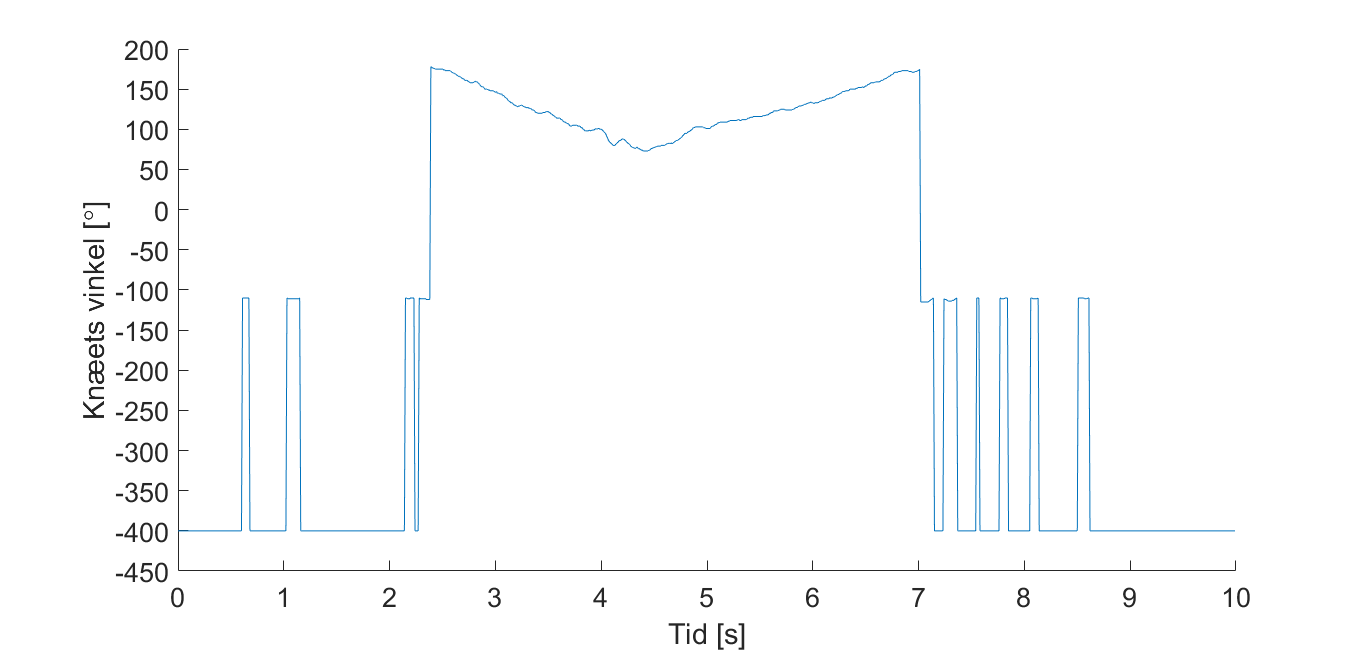
\includegraphics[width=1\textwidth]{figures/vinkeltest_graenser}
\caption{Grafen illustrerer vinklen over knæet under en squat-øvelse. En vinkel under $-100^{\circ}$ symboliserer en overskridelse af $180^{\circ}$ over knæleddet.}
\label{fig:vinkeltest_graenser}
\end{figure}

\noindent
Det ses på \autoref{fig:vinkeltest_graenser}, at forsøgspersonen overstrækker knæleddet de første $2~s$, således begge accelerometre overstiger grænsen på $90^{\circ}$, der tilsammen udgør en vinkel på $180^{\circ}$. 
Dette visualiseres ved en vinkel på $-400^{\circ}$. 
Efter 0,5 sekunder ses en vinkel på $-110^{\circ}$, hvilket er gældende, da det ene accelerometer har haft en spænding svarende til præcis $90^{\circ}$ og har derfor ikke overskredet grænsen. 
Ved squat-øvelsens begyndelse falder vinklen fra $180$ til $73^{\circ}$, hvorefter den stiger til $180^{\circ}$. 
Til slut i målingen ses igen et fald under $-100^{\circ}$, hvilket indikerer, at forsøgspersonen igen overstrækker knæleddet.

\noindent
En yderligere test er foretaget for at undersøge forsinkelsen, og følger samme anvisninger beskrevet i \autoref{sec:lavpas_test}.  
Resultatet af denne test giver en forsinkelse på  $3,6~\mu s$. Dette betragtes ikke som værende af signifikant betydning i forhold til det samlede system, hvorfor denne forsinkelse accepteres.


\vspace{3mm}
\textbf{Opsummering af krav:}
\begin{itemize}
%\item[\text{\sffamily \checkmark}] Skal kunne udregne en samlet vinkel over knæet
\item[\text{\sffamily \checkmark}] Skal kunne udregne knæets vinkel indenfor intervallet $90-180^{\circ}$
\begin{itemize}
\item Dette skal indikeres ved en grøn LED
\end{itemize}
\item[\text{\sffamily \checkmark}] Skal indikere, hvornår knæets vinkel er udenfor intervallet $90-180^{\circ}$
\begin{itemize}
\item Dette skal indikeres ved en rød LED
\item Hvis vinklen for ét accelerometer overstiger $90^{\circ}$, indikeres dette som et output på $-200^{\circ}$, hvortil det andet accelerometers vinkel lægges til de $-200^{\circ}$
\item Hvis vinklen overstiger $90^{\circ}$ for hvert accelerometer, skal dette indikeres som et output på $-400^{\circ}$
\end{itemize}
\end{itemize}
\subsection{EMG-algoritme}
For at undersøge, om kravene i \autoref{sec:krav_emg_algo} opfyldes, testes EMG-algoritmen ved et muskelsignal på 10 sekunder, der varierer i amplitude. Inputtet til algoritmen, det filtrerede muskelsignal, og outputtet vælges til at være henholdsvis $-10$ eller $10$, hvis muskelsignalet er faldende eller stigende. Derudover ønskes det at outputsignalet er 0, hvis der opnås en vinkel på under $90$ eller over $180^{\circ}$. Dette illustreres ved hjælp af MATLAB på \autoref{fig:emg_algo_test}. 

\begin{figure}[H]
\centering
\includegraphics[width=0.9\textwidth]{figures/EMG_algo_test}
\caption{Den blå graf og tilhørende venstre y-akse illustrerer det filtrerede muskelsignal, der er EMG-algoritmens input, og den røde graf og tilhørende højre y-akse illustrerer, om muskelsignalet er henholdsvis faldende eller stigende ved enten at udsende et signal på $-10$ eller $10$.}
\label{fig:emg_algo_test}
\end{figure}

\noindent
Ud fra de data, der fremgår af \autoref{fig:emg_algo_test}, findes EMG-inputtets lokale minima- og maksimapunkter. Tidspunkterne for disse lokale ekstrema sammenlignes med tidspunkterne, hvor outputtet skifter i spænding ved at udregne en forsinkelse i sekunder ud fra differensen på tidspunkterne for det lokale ekstrema og skift i output. Dette fremgår af \autoref{tab:emg_algo}. 

\begin{table}[H]
\centering
\begin{tabular}{|c|c|c|}
\hline 
\textbf{EMG-ekstrema [s]} & \textbf{Output[s]} & \textbf{Forsinkelse [s]}\\ 
\hline 
0,32 & 0,32 & 0,00\\ 
\hline 
0,79 & 0,80 & 0,01\\ 
\hline 
0,85 & 0,86 & 0,01\\ 
\hline 
1,02 & 1,03 & 0,01\\ 
\hline 
1,11 & 1,12 & 0,01\\ 
\hline 
1,51 & 1,52 & 0,01\\ 
\hline 
2,48 & 2,49 & 0,01\\ 
\hline 
2,67 & 2,68 & 0,01\\ 
\hline 
2,95 & 2,96 & 0,01\\ 
\hline 
3,53 & 3,54 & 0,01\\ 
\hline 
3,62 & 3,63 & 0,01\\ 
\hline 
3,97 & 3,98 & 0,01\\ 
\hline 
4,33 & 4,34 & 0,01\\ 
\hline 
4,69 & 4,70 & 0,01\\ 
\hline 
5,04 & 5,05 & 0,01\\ 
\hline 
5,50 & 5,51 & 0,01\\ 
\hline 
5,68 & 5,69 & 0,01\\ 
\hline 
5,88 & 5,89 & 0,01\\ 
\hline 
7,53 & 7,54 & 0,01\\ 
\hline 
8,49 & 8,50 & 0,01\\ 
\hline 
8,84 & 8,85 & 0,01\\ 
\hline 
9,00 & 9,01 & 0,01\\ 
\hline 
9,08 & 9,09 & 0,01\\ 
\hline 
\end{tabular} 
\caption{Tabel over ekstrema, outputskift og differensen mellem disse, der er noteret som forsinkelsen.}
\label{tab:emg_algo}
\end{table}

\noindent
I \autoref{tab:emg_algo} fremgår det, at forsinkelsen fra inputtet af muskelsignalet, der registreres som en ændring i output-signalet, er mellem $0,00$ og $0,01~s$. Den gennemsnitlige forsinkelse er dermed på $9,57~ms$. Målingen, der giver en forsinkelse på $0,00~s$, kan dog ikke passe, da EMG-algoritmen bruger én sample på at skifte output fra $10$ til $-10$ eller fra $-10$ til $10$. Ingen forsinkelse vil derfor betyde, at EMG-algoritmens output begynder at ændre sig fra $-10$ til $10$, før EMG-signalet er begyndt at stige. 

Forsinkelsen på $9,57~ms$ kan forklares af, at testen er udført ved at sample EMG-algoritmens input og output ved $100~Hz$. Af denne grund er der ikke mere end 100 samples per sekund, hvilket betyder, at der er $10~ms$ mellem hver sample. Forsinkelsen er derfor sandsynligvis mindre end $9,57~ms$, men det kan ikke lade sig gøre at måle mindre tal med den nuværende samplerate. 

\vspace{3mm}
\textbf{Opsummering af krav:}
\begin{itemize}
\item[\text{\sffamily \checkmark}] Skal kunne detektere om muskelaktiviteten er faldende eller stigende mellem to samples med 0,01 sekunders mellemrum
\begin{itemize}
\item Ved stigende muskelaktivitet skal dette indikeres som et outputsignal på $+10$
\item Ved faldende muskelaktivitet skal dette indikeres som et outputsignal på $-10$
\end{itemize}
\item[\text{\sffamily \checkmark}] Skal kunne indikere, hvis vinklen befinder sig udenfor intervallet $90-180^{\circ}$
\begin{itemize}
\item Dette skal indikeres ved, at outputsignalet går i $0$
\end{itemize}
\end{itemize}
\subsection{Trådløs kommunikation}
Den trådløse kommunikation testes for at undersøge, hvorvidt kravene opstillet i \autoref{sec:traadloes_komm_design} opfyldes. 

\noindent
Kravet for, at USB-donglen skal forsynes via USB opfyldes ved måden, hvorved den trådløse kommunikation er implementeret. Her er BLE-donglen erstattet med en alternativ modtagerenhed som beskrevet i \autoref{traadloes_komm_imp}, og denne tilsluttes en computer via USB, hvorfra den forsynes. 

%\noindent
%Til test af forsinkelse for transmission, defineres en debug pin på mikrokontrolleren og på modtagerenheden. Når data transmitteres sættes pin'en på mikrokontrolleren høj, samt på modtagerenheden, når data modtages. Hertil kan der via et oscilloscope aflæses en forsinkelese mellem de to pin. 

\noindent
Til test af afstand, programmeres mikrokontrolleren til at transmittere en værdi, der tæller op fra nul. Denne værdi transmitteres 10 gange i sekundet til en computer, hvorpå denne data visualiseres i programmet Realterm.
Startpunket for testen er med en afstand på $1~m$ mellem modtagerenheden på computeren og mikrokontrolleren. 
Hertil øges afstanden med $1~m$ indtil der opnås en afstand svarende til det opstillede krav på $2~m$. Yderligere fortsættes forøgelsen af afstanden op til maks $4~m$, eller til der ikke længere modtages data. Dette er for at undersøge om de $2~m$ markerer grænsen for den tråløse kommunikation, og dermed definere et flexområde i forhold til det opstillede krav. Testen udføres under forhold, hvor der er fri passage mellem mikrokontroller og modtager.  

\begin{table}[H]
\centering
\begin{tabular}{|c|c|}
\hline 
Afstand [m] & Gennemført transmission \\ 
\hline 
1 & Ja \\ 
\hline 
2 & Ja \\ 
\hline 
3 & Ja \\ 
\hline 
4 & Ja \\ 
\hline 
\end{tabular} 
\caption{Data over afstandstest for den trådløse kommunikation. Venstre søjle oplyser afstand mellem mikrokontroller og modtagerenhed. Den højre oplyser, hvorvidt transmissionen har været succsesfuld eller ej.}
\label{tab:traadloes_komm_test_afstand}
\end{table}

Ud fra \autoref{tab:traadloes_komm_test_afstand} kan der konkluderes et flexrum for den trådløse kommunikation, der er $100~\%$ af det opstillede krav. Yderligere viste testen, at systemet lagrer data i en buffer i tilfælde af, at forbindelsen blev afbrudt. I det forbindelsen blev genetableret, blev den tabte data transmitteret, således ingen data gik tabt. Det kan derfor ligeledes konkluderes, at de opstillede krav for trådløs kommunikation opfyldes.

\textbf{Opsummering af krav:}
\begin{itemize}
\item[\text{\sffamily \checkmark}] Mikrokontrolleren skal kommunikere trådløst med en computer
\item[\text{\sffamily \div] BLE-dongle skal forsynes via USB
\begin{itemize}
\item[\text{\sffamily \checkmark}] En anden modtagerenhed er implementeret, hvilket forsynes via USB
\end{itemize}
\item Skal have en maksimal forsinkelse på 100 ms \fxnote{skal denne forsinkelse være større eller mindre?? - HUSK at ændre i brødteksten også!}
\item Skal have en kommunikationsrækkevidde på $2~m$
\end{itemize}
%Kommunikation med NXT:
  
%%-----------------------Systemtest-------------------------%%
\chapter{Systemtest}
Dette kapitel indeholder beskrivelse, udførsel af test samt konklusion for test af systemet med kendt input og et bruger-input. 

\section{Systemtest med kendt input} \label{sec:test_kendtinput}
I dette afsnit vil det samlede system testes, således det er muligt at undersøge, om systemet behandler inputs som forventet. På baggrund af disse målinger er det muligt at konkludere, hvorvidt systemet virker. 

\subsection{Beskrivelse}
For at simulere accelerometresignaler anvendes to spændingsforsyninger til at repræsentere accelerometrene. Spændingen varieres over tid, således denne svarer til en samlet vinkel mellem $90-180^{\circ}$. Derudover testes det, om vinklen vil falde til $-200^{\circ}$ for hvert accelerometer, når spændingen svarende til $180^{\circ}$ overskrides. 

For at teste det samlede system med et kendt input benyttes en funktionsgenerator, således et $500~Hz$ sinussignal med en peak-peak-amplitude på $4~mV$ kan genereres. Sinussignalets frekvens og amplitude er omkring, hvad der kan forventes af et EMG-signal. Outputtet fra sinussignalet er filtreret gennem det implementerede digitale lavpasfilter. 

Testen foretages over 10 sekunders måling og samples via mikrokontrolleren. Ud fra disse målinger, er det muligt at teste systemets blokke, når de er sammensat. Dette gøres ved at sammenligne input og output af det samplede sinussignal samt spændingerne for acclerometrene omregnet til en samlet vinkel.


\subsection{Resultater af test}
Fra testen plottes og visualiseres systemets input af det samplede sinussignal, output fra det opsamlede digitalt filtrerede signal samt spændingen fra de to accelerometre, der er omregnet til en samlet vinkel ved lineær interpolation. Derudover er det opsamlede digitale output, som er behandlet i EMG-algoritmen, plottet. Resultaterne fremgår af \autoref{fig:test_kendtinput}. 

\begin{figure}[H]
\centering
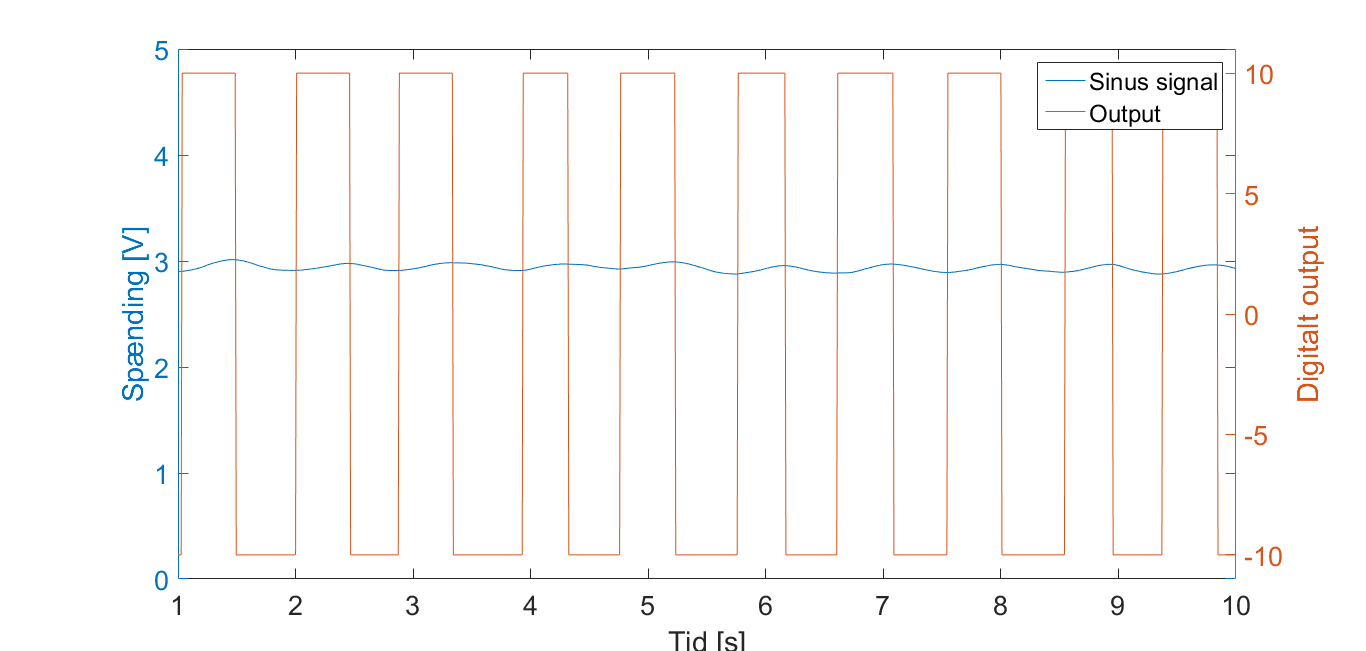
\includegraphics[width=1\textwidth]{figures/kontrol_test_sinus}
\caption{På den øverste graf illustreres den samlede vinkel over tid. Det fremgår af grafen, at vinklen er stigende fra $90^{\circ}$ til $175^{\circ}$, hvorefter vinklen falder til $-115^{\circ}$. Dette skyldes en overskridelse af spændingen for accelerometeret svarende til $180^{\circ}$.
På den midterste graf illustrerer den blå graf det opsamlede inputsignal, svarende til en sinus på $500~Hz$ med en $V_{pp}$ på $4~mV$. Den røde graf illustrerer det samplede sinussignal med et implementeret digitalt lavpasfilter, disse værdier er målt i spænding. 
På den nederste graf illustreres signalets digitale output. Signalet går fra $+10$ ved stigende muskelaktivitet til $-10$ ved en faldende muskelaktivitet. Grafen går i $0$, når en vinkel udenfor $90-180^{\circ}$ opnås.}
\label{fig:test_kendtinput}
\end{figure}

\noindent
På baggrund af målingerne for den øverste graf på \autoref{fig:test_kendtinput} fremgår det, at en indsendt stigende spænding svarende til $90-175^{\circ}$, får det den samlede vinkel til at stige. Ved en vinkel på $175^{\circ}$ overskrider det ene accelerometer dens maksimale spænding, hvorfor vinklen falder til $-115^{\circ}$ over $1~ms$. 

Dette burde ifølge den implementerede kode gå ned til en vinkel på $-200^{\circ}$ ved overskridelse af vinklerne, hvori EMG-algoritmen fungerer. 
At vinklen ikke når en samlet værdi på $-400^{\circ}$ er en indikatior for, at det ene accelerometers spænding har været inden for algoritmens grænser, mens det andet accelerometer har overskredet grænserne. Hertil kan det ses, at det ene accelerometer har haft en outputspænding svarende til $85^{\circ}$, mens det andet accelerometer har haft en spænding, der har overskredet grænsen og derfor har en vinkel på $-200^{\circ}$.

Det fremgår af den midterste og nederste graf på \autoref{fig:test_kendtinput}, at der ses en sammenhæng mellem det opsamlede digital filtrerede sinussignal og det opsamlede outputsignal. Ved et stigende sinussignal vil outputsignalet indikere $+10$, hvilket svarer til en positiv hældning af sinussignalet. Ved en negativ hældning af sinussignalet vil outputsignalet indikere et fald og dermed give et output på $-10$.

På den nederste graf på \autoref{fig:test_kendtinput} fremgår det, at efter outputsignalet har befundet sig i $-10$ ved $9~s$, stiger outputsignalet efterfølgende til $0$. Dette er grundet, at de samlede grader har overskredet én eller flere grænser, og derved fungerer EMG-algoritmen ikke, hvilket illustreres ved, at outputsignalet er $0$.

Der er yderligere foretaget en test af det samlede forsinkelse på systemet uden trådløs kommunikation. Denne test blev udført på samme måde som i \autoref{sec:lavpas_test}. Resultaterne for forsinkelse blev målt til $832~\mu s$ for det samlede system testet uden trådløs kommunikation. 
\section{Systemtest med bruger-input}

\subsection{Beskrivelse}
For at teste det samlede system med bruger-input påsættes den positive og negative elektrode på femur, og referenceelektroden påsættes anklen, som illustreret i \autoref{sec:pilotforsoeg} på henholdsvis \autoref{fig:laarmuskler} og \autoref{fig:reference}, ud fra SENIAMs anvisninger \citep{seniam2016}. Huden præpareres inden dette for, således at fjerne hår og døde hudceller. 
De to accelerometre påsættes breadboards for at stabilisere deres placering, disse placeres henholdsvis parallelt med femur og tibia, som illustreret på \autoref{fig:accelerometervinkel}.

Systemet testes over 10 sekunders måling, hvor forsøgspersonen udfører en squat-øvelse. Der skal hertil foretages to målinger, hvor forsøgspersonen starter med at overskride 180$^{\circ}$ af knæet ved at overtrække knæleddet. Herefter bevæger forsøgspersonen sig langt ned i en squat-øvelse, hvorved vinklen af knæet overskrider grænsen på 90$^{\circ}$. Forsøgspersonen bevæger sig herefter tilbage til udgangsposition, hvorved de 180$^{\circ}$ overskrides ved overstræk af knæleddet.
På denne måde testes det, hvorvidt om det samlede system fungerer, da en overskridelse af $90-180^{\circ}$ vil betyde, at data ikke vil gå videre ind i EMG-algoritmen. Dette illustreres ved at det digitale output vil være i 0. Under testen opsamles det samplede digital filtrede EMG-signal, EMG-algoritmen samt vinklen over knæet.

\subsection{Resultater af forsøg}
På baggrund af testen er der plottet og visualiseret systemets input samt output. Visualiseringen forekommer af \autoref{fig:test_brugerinput}. 
 
\begin{figure}[H]
\centering
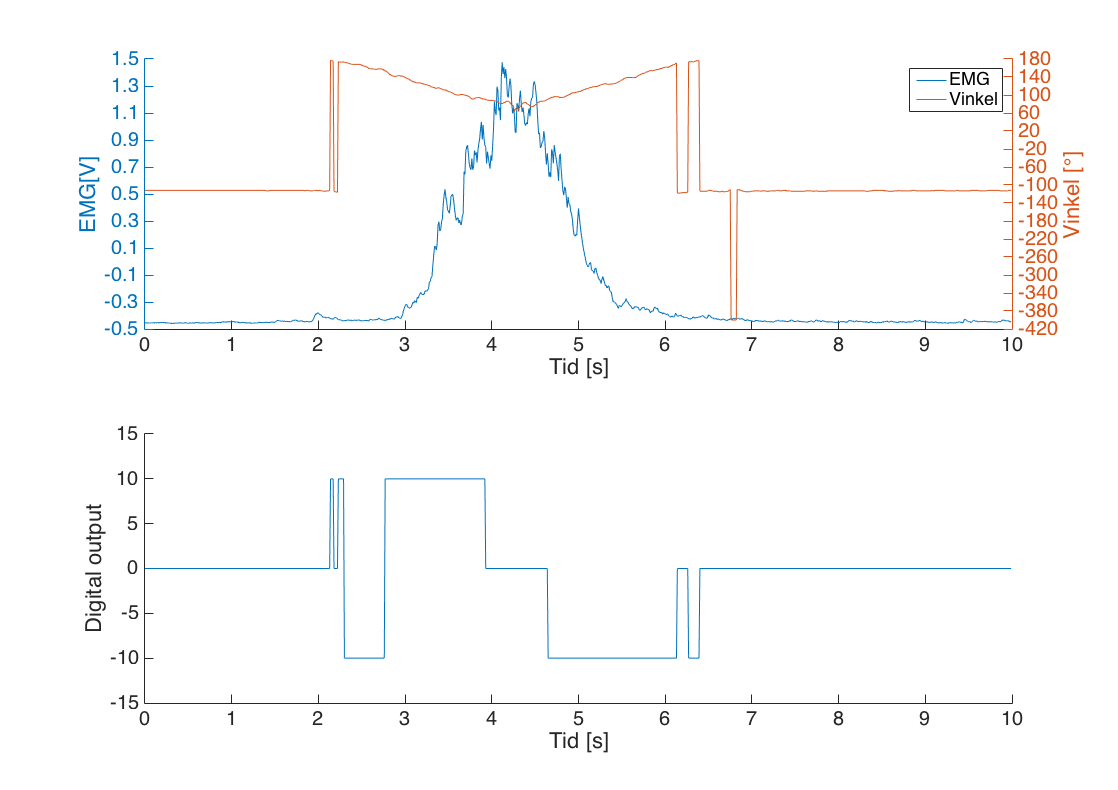
\includegraphics[width=0.4\textwidth]{figures/test_brugerinput}
\caption{På den øverste figur ses muskelaktivitet ved udførelse af en squat-øvelse, samt vinklen over knæet under øvelsen. Den blå graf illustrerer det samplede digital filtreret EMG og den røde graf illustrerer vinklen over knæet. Hertil ses der fald ned til under 0$^{\circ}$, hvilket illustrerer en overskridelse af $180^{\circ}$. Den nederste figur illusterer signalets digitale output i EMG-algoritmen. Denne visualiserer en stigning og et fald af det opsamlede EMG-signal, hvorved en stigning af muskelaktiviteten illustreres som værende $+10$ og et fald i muskelaktiviteten som værende $-10$. Ved grafen lig 0 illustreres en overskridelse af $90-180^{\circ}$ af knæet.}
\label{fig:test_brugerinput}
\end{figure}

Ud fra testen ses der en sammenhæng mellem muskelaktiviteten under en squat-øvelse og vinklen over knæet under øvelsen. Ved en stigning af muskelaktiviteten ses et fald i grader over knæet, hvilket ses mellem $2-4~s$. Hvorved der ved fald af muskelaktiviteten ses en stigning af grader, dette ses mellem $4,5-6,5~s$.
Ved starten af øvelsen overstrækker forsøgspersonen knæet, hvilket ses ved, at vinklen er $-112^{\circ}$. Grunden til denne er $-112^{\circ}$ og ikke $-400^{\circ}$ er, at det ene accelerometer har været indenfor græsen på $180^{\circ}$ og den andet accelerometer har overskredet grænsen. Det samme gør sig gældende ved slutningen af øvelsen. Ved overstrækning af knæet og dermed overskridelse af $180^{\circ}$ ses EMG-algorimten værende 0. 
Efter $2~s$ overstrækkes knæet ikke længere og graderne begynder derved at falde i takt med muskelaktiviteten stiger. Ved en stigning af muskelaktiviteten ses EMG-algorimten ligeledes stigende. Ved $4~s$ er vinklen over knæet $81^{\circ}$, hvilket er en overskridelse af grænsen på $90^{\circ}$. Dette illustreres ved EMG-algoritmen går i 0. 
Efter $4,5~s$ ses en stigning af grader i takt med et fald i muskelaktiviteten. Derved ses der ligeledes et fald i EMG-algoritmen. 
Efter $6~s$ overstrækkes knæene igen, hvorefter begge accelerometre overskrider deres grænser, derfor går grafen i $-400^{\circ}$. Herefter overstrækkes knæene fortsat, dog ligger det ene accelerometer indenfor dens grænse, hvilket forklarer vinklen på $-112^{\circ}$. 




\subsection{Konklusion}

\section{Konklusion af systemtest}
....gfghhd



%%-----------------------Syntese-------------------------%%
\chapter{Syntese}
\section{Diskussion}
Formålet med dette projekt er at udvikle et system, som kan opsamle signaler fra kroppen, hvor der er fokus på digital signalbehandling og datakommunikation \citep{aalborguniversitet2014}. På baggrund af dette er der udviklet et system, der kan måle muskelaktivtet fra rectus femoris ved hjælp af EMG og måle vinklen over knæet ved hjælp af accelerometre, og som har til formål at støtte knæets omkringliggende muskler, så ALS-patienter støttes i forbindelse med udførelsen af en squat-øvelse. På baggrund af teori, implementering og test af systemets enkelte blokke fremgår det, at kravene til de enkelte blokke er overholdt. Der er dog nogle områder, hvor andre alternativer kan overvejes for mulige forbedringer af hele systemet. 

\subsection{Implementering}
Systemet er udviklet, så størstedelen af signalbehandlingen foregår digitalt, da dette er fokus i forhold til studieordningen. Hvis dette ikke havde været et krav for dette semester, kunne det have været en fordel, at nogle af blokkene var designet analogt, hvorved det kunne være nemmere at finde samt rette op på eventuelle fejl i systemet. Et eksempel herpå er i forhold til opsamling af signaler fra accelerometre. 

For at give en bedre opløsning af accelerometrene kunne det være relevant at implementere en forstærker inden ADC'en, hvorved der opnås en bedre repræsentation af accelerometersignalerne. Denne forstærker blev ikke implementeret, da det ville kræve en analog offsetjustering af signalet, så signalet ikke vil gå i mætning, da signalet med offset vil kunne overstige ADC'ens arbejsområde. %. Offsettet er teoretisk ved en påvirkning af $0~g$ den halve spændingsforsyning. Uden denne offsetjustering vil det kunne resultere i, at signalet vil gå i mætningen, da dette vil kunne overstige ADC'ens arbejdsområde alt efter hvor meget signalet forstærkes, hvorved der yderligere skal tages højde for denne parameter.

%Der kunne i stedet for accelerometrene være implementeret andre sensorer til vinkelmåling - eksempelvis gyroskop eller et goniometer. Ved et gyroskop anvendes impulsmomentbevarelse, hvorved det kan udregnes hvor meget patienten har bevæget sig under en squat-øvelse. Ved goniometer er det muligt at se, hvilken vinkel knæet har i oprejst position og hvor meget det så har bevæget sig. Da der ønskes at beregne vinklen gennem hele øvelsen, blev disse sensorer fravalgt. Udover disse kriterier  var accelerometrene også til rådighed. Da det er muligt at videreudvikle systemet så det kan benyttes under gang, vil det også være fordelagtigt at anvende accelerometre, det skal dog vurderes om der skal anvendes andre, da det kræver at accelerometrene har et større arbejdsområde end $\pm3~g$.

Systemet benytter herudover en udleveret komponent, EMG-forstærkeren, der ensretter, forstærker og envelopefiltrerer signalet. Denne blok kunne være fordelagtig at implementere som flere blokke, så det ville være muligt at teste og dokumentere disse hver for sig. På denne måde vil det være muligt at opstille krav til hver blok og justere og ændre disse blokke. Dette vil dog ikke påvirke systemet, som det er nu, da EMG-forstærkeren opfylder de opstillede krav. %Dog vil  eventuelle forsinkelser og ændringer ikke have den store betydning ved at anvende EMG-forstærkeren, da signalet er meget lavfrekvent og det vil derfor ikke have en betydning for repræsentation af muskelaktiviteten. 

I projektet er der valgt at anvende trådløs kommunikation, så ledninger ikke vil være til gene for brugeren af systemet. Dog har d hvilket kan få betydning for den videre kommunikation og udførelse. En løsning på dette vil være ikke at koble de enkelte komponenter til det samme baseboard, men i stedet koble dem mellem hinanden, hvorved der ikke længere er en en trådløs forbindelse. Denne løsningsmetode vil kunne give nogle begrænsninger i forhold til rækkevidde, hvilket også vil kunne ske ved den trådløse kommunikation, hvorfor dette ikke vurderes at være et større problem i forhold til implementering. 


%\subsection{Batteridrevet}
%På nuværende tidspunkt er systemet batteridrevet, hvorfor der skal tages højde for batteriets levetid og hvorvidt det er muligt at forlænge battieriets levetid og dermed gøre systemet så effektivt som muligt. (skriv mere..)

%\subsection{Videreudvikling}
%Systemet vil ikke være anvendeligt for ALS-patienter på nuværende tidspunkt, da systemet ikke er færdigudviklet. En prototype af systemet ved anvendelse af et exoskelet vil støtte musklerne omkring knæet under udførelse af squat-øvelse. 

%På baggrund af det udviklede systemet, vil det være muligt at videreudvikle systemet, så det kan støtte benmuskulaturen under gang, hvorved det vil være mere essentielt at anvende for ALS-patienter. For at kunne udvikle sådan et system skal flere ukendte parametre, som kan variere fra patient til patient undersøges. Systemet ses som en hjælp til brugeren, da det ikke vil yde nogen behandling. 

%\subsection{Brugervenlighed}
%For at systemet er mere brugervenligt, er der implementeret LED'er som viser brugeren, hvornår knæet har bevæget sig over eller under den valgte vinkel på henholdsvis $90^{\circ}$ og $180^{\circ}$. For at optimere brugervenligheden kunne dette også gøres ved at indføre vibration, som oplyser patienten om dette, hvilket vil være mere optimalt, da patienten ikke kan ses LED'erne under øvelsen. Samtidig kunne denne besked blive sendt til brugeren inden grænsen er overskredet for at advare brugeren. 

%Derudover har systemet en start- og stopfunktion. Dette kan både være en fordel og ulempe for brugeren. Det vil være nødvendigt at skulle starte og stoppe hver gang systemet skal anvendes, hvilket kan være til gene for brugeren over en længere tidsperiode. Det vil være fordelagtigt, da gør det muligt for brugeren selv at bestemme, hvornår øvelsen skal starte og stoppe.

\subsection{Samlet systemtest}
\section{Konklusion}

I dette projekt er der udviklet et digitalt system, der kan optage muskelsignaler fra rectus femoris samt signaler fra accelerometrene. Muskelsignalerne viser, hvorvidt muskelsignalerne er stigende eller faldende samtidig med, at signalerne fra accerelerometrene anvendes til beregning af vinklen over knæet under en squat-øvelse. Systemet er udviklet med henblik på at kunne hjælpe ALS-patienter til aflastning af muskulaturen omkring knæet. Systemets blokke, der består af opsamling af signaler, spændingsforsyning, ADC, digital filtrering, vinkelberegning, EMG-algoritme og trådløs kommunikation er designet, implementeret samt testet. Disse blokke evalueres ud fra testene for at vurdere, hvorvidt de opstillede kravspecifikationer for blokkene opfyldes. Ud fra dette ses det, at kravet for trådsløs kommunikation mellem mikrokontrolleren og LEGO mindstorm NXT ikke opfyldes, samt kravet om en maksimal forsinkelse på 100 ms ikke er opfyldt. Det kan ud fra evalueringen af testene konkluderes, at de resterende kravspecifikationer for de enkelte blokke er opfyldt. 

Det samlede system er herefter testet med et kendt inputsignal samt et inputsignal fra en bruger. Denne test viser, at systemet fungerer som ønsket. En prototype i form af et exoskelet er ikke udviklet, hvorfor dette krav ikke er opfyldt. Det vil på baggrund af dette, på nuværende tidspunkt, ikke være muligt at anvende systemet som bodyaugmentation som hjælpemiddel til ALS-patienter. 

For at kunne styre samt anvende et exoskelet under en squat-øvelse benyttes signalerne fra accelerometrene samt muskelsignalerne fra. Ud fra signalerne fra accelerometeret beregnes den samlede vinkel over knæet. Når denne vinkel befinder sig mellem  $90^{\circ}$ og $180^{\circ}$, vurderes det ud fra muskelaktiviteten om brugeren bevæger sig i en opadgående eller nedadgående retning. Herved vil disse informationer sendes trådløst til et exoskelet for således at kunne anvende dette system som bodyaugmentation til ALS-patienter.
\section{Perspektivering}
I dette afsnit vil projektet perspektiveres for at reflektere over de forskellige aspekter, der bør undersøges for at skabe et færdigudviklet produkt, der kan anvendes af ALS-patienter. 

Systemet er udviklet til at kunne hjælpe ALS-patienter ved at aflaste deres lårmuskulatur under en squat-øvelse. Der er ikke udviklet en prototype, der skal kunne muliggøre dette, hvorfor systemet skal videreudvikles, således det er anvendeligt uden at være til gene for brugeren. Systemet optimeres og forbedres på flere områder, da det har nogle begrænsninger, der betyder, at systemet ikke kan anvendes ved en vinkel over $180^{\circ}$ og under $90^{\circ}$. Dette skaber derfor nogle begrænsninger for brugerens bevægelig. Herudover vil det være fordelagtigt at sende en advarsel inden grænserne på $180^{\circ}$ og  $90^{\circ}$ er overskrevet i form af en vibration. Brugeren skal på nuværende tidspunkt selv starte og stoppe systemet, hvilket kan videreudvikles til en automatisk funktion, når brugeren udfører en bevægelse.  


Ydermere vil systemet kunne videreudvikles, således det vil være muligt at anvende under gang for ALS-patienter, og derved støtte deres muskulatur, da det på nuværende tidspunkt kun er muligt at udføre en squat-øvelse. En implementering i forhold til sikkerhed kan være en udvikling, hvor en alarm starter i tilfælde af, at brugeren mister balancen eller falder under gang. 






%\iffalse
\begingroup
\raggedright

\bibliographystyle{unsrtnat}
\bibliography{kilder}

\endgroup

%-----------------------Bilag-------------------------
\appendix
%\chapter{Bilag}
\section{Pilotforsøg}
%Nirushas udgave
I dette projekt udføres et pilotforsøg for identificering af støj samt andre uønskede signaler ved anvendelse af sensorer. Pilotforsøget danner grundlag for optimering af kravspecifikationerne i de forskellige blokke. Herudover undersøges elektrodernes placering for at opnå det bedst mulige signal under udførelse af en squat-øvelse.
%Signes udgave
I dette projekt udføres et pilotforsøg for identificering af støj samt andre uønskede signaler ved anvendelse af sensorer. Pilotforsøget danner grundlag for optimering af kravspecifikationerne i de enkelte blokke. Derudover undersøges det, hvor elektroderne skal placeres for at opnå det bedst mulige signal under udførelse af en squat-øvelse.


\subsection{Formål}
Der anvendes en EMG-forstærker og et accelerometer som sensorer. På baggrund af dette opstilles følgende formål for de enkelte sensorer.  

\subsubsection{EMG-forstærker}
\begin{enumerate}
\item Opsamling af signal fra rectus femoris og biceps femoris
\begin{itemize}
%Nirushas udgave
\item Identificering af elektrodernes placering
\item Sammenligning af muskelaktivitet under en squat-øvelse 
%Signes udgave
\item Identificere placeringen af elektroder
\item Sammenligne muskelaktivitet oprejst og i en squat-øvelse 

\end{itemize}
\item Identificering af støjsignaler
\end{enumerate}


\subsubsection{Accelerometer}
\begin{enumerate}
%Nirushas udgave
\item Identificering af position under en squat-øvelse
\item Identificering af støjsignaler
%Signes udgave
\item Identificere position af knæleddet siddende i en squat-øvelse
\item Identificere støj ved opsamling af signaler

\end{enumerate}


\subsection{Materialer} 
\begin{itemize}
\item EMG-forstærker
\item Elektroder
\item Desinfektionsservietter
\item Skraber
\item Tusch 

\item Accelerometer ADXL335Z
\item Tape
\item Ledninger

\item Computer
\item CY8CKIT-042-BLE
\end{itemize}

\subsection{Metode}

%Nirushas udgave
For at identificere den bedste mulige elektrodeplacering optages EMG signaler fra forskellige placeringer på de to muskler. 
For at simulere den påvirkning som accelerometeret udsættes for og derved identificere det maksimale og minimale outputsignal roteres accelerometeret i en langsom rotation fra 0 $^{\circ}$ til 90 $^{\circ}$ til både højre og venstre. Herudover måles accelerometerets påvirkning i henholdsvis 0 og 1 g-påvirkning, for at identificere accelerometeres påvirkning og hvorledes dette stemmer overens med databladet. 
For at identificere støj fra EMG forstærkeren optages aktivitet i musklerne under en squat-øvelse.
 
%Signes udgave
For at identificere den bedste placering af elektroder optages EMG-signaler fra forskellige placeringer på de to muskler. 
For at simulere den påvirkning som accelerometeret udsættes for og derved identificere det maksimale og minimale outputsignal roteres accelerometeret i en langsom rotation fra 0 $^{\circ}$ til 90 $^{\circ}$  til både højre og venstre. Herudover måles accelerometeret påvirkning i henholdsvis 0 og 1 g-påvirkning for at identificere accelerometeres påvirkning og hvorledes dette stemmer overens med databladet. 
For at identificere støj fra EMG-forstærkeren optages aktivitet i musklerne i en squat-øvelse.


\subsection{Forsøgsopstilling}
Forsøgsopstilling er for den primære udførelse af forsøget. Nogle af processerne gentages for at kunne sammenligne de forskellige målinger, og derved få et bedre resultat.

%Nirushas udgave
\subsubsection{EMG-forstæker}
Rectus femoris og biceps femoris identificeres, den ønskede placering af elektroderne markeres med tusch. Herefter fjernes eventuelle hår og døde hudceller ved brug af skraber. Huden desinficeres herefter ved brug af desinficeringsservietter og elektroderne påsættes. Den røde ledning påsættes rectus femoris/bicep femoris og den grønne ledning påsættes rectus femoris/bicep femoris. Den sorte ledning påsættes (tibia) og anvendes som referencepunkt.
%Signes udgave
\subsubsection{EMG-forstæker}
Rectus femoris og biceps femoris identificeres, den ønskede placering af elektroderne markeres med tusch. Herefter fjernes eventuelle hår og døde hudceller ved brug af skraber. Huden desinficeres herefter ved brug af desinficeringsservietter og elektroderne påsættes. Den røde ledning påsættes rectus femoris/bicep femoris og den grønne ledning påsættes rectus femoris/bicep femoris. Den sorte ledning påsættes patella og anvendes som referencepunkt.


\subsubsection{Accelerometer}
Accelerometeret påsættes siden af låret, så accelerometer måles i xyz-plan, hvorved der måles i den vertikale retning. Der sørges for,  at accelerometeret befinder sig i 0 g påvirkning ved starten af forsøgets udførelse, hvorved accelerometeret er kaliberet. 

\subsubsection{Opstilling}
\begin{itemize}
\item Identificering af musklerne rectus femoris og biceps femoris 
\item Elektrodernes placering markeres
\item Huden skrabes og desinficeres
\item Elektroderne påsættes
\item Ledningerne påsættes elektroderne
\begin{itemize}
\item Den røde/grønne ledning på rectus femoris
\item Den røde/grønne ledning på biceps femoris
%Nirushas udgave
\item Den sorte ledning/reference på tibia??
%Signes udgave
\item Den sorte ledning/reference på patella \fxnote{positiv/negativ/ground}

\end{itemize} 
\item Accelerometeret på sættes patella ved en 0 g påvirkning i x,y,z retning
\end{itemize}


\subsection{Fremgangsmåde}
Fremgangsmåden udføres XX antal gange, hvorved der på baggrund af målingerne foretages en gennemsnitsværdiberegning.
%Nirushas udgave
\subsubsection{EMG/EMG forstærker}
EMG måling: Squat-øvelsen starter stående, hvorefter forsøgspersonen langsomt udføre bevægelsen og dermed kommer ned i en dybere squat, hvor der undervejs foretages målinger.
%Signes udgave
\subsubsection{EMG/EMG-forstærker}
EMG måling: 10-sekunders målinger trinvist under udførelse af en squat-øvelse. 


\subsubsection{Accelerometer}
Påvirkning i 0 og 90 $^{\circ}$.
Påvirkning af rotation fra 0 til 90 $^{\circ}$ til både højre og venstre.
Optag 30 sekunder ved 0 og 90 $^{\circ}$ .
Optag rotation: baseline 10 sekunder, rotation 10 sekunder, baseline 10 sekunder





\section{Test af accelerometer} 
\label{sec:test_acc}
I dette projekt anvendes to accelerometre, som er beskrevet i \autoref{sec:acc}. Disse anvendes som sensorer til opsamling af acceleration, der giver et outputsignal svarende til en spænding. For at kunne anvende et accelerometer er det vigtigt at kende forskellige tolerancer i forhold til deres datablade, hvorfor et forsøg udføres for at kunne tage højde for disse parametre.

\subsection{Formål}\label{sec:acc_formaal}
Denne test har til formål at identificere en given spændingen for forskellige vinkler. Derudover identificeres %støjsignaler i outputsignalet samt 
offsettet og sensitiviteten for at teste accelerometrenes tolerancer.

\begin{enumerate}
%\item Identificering af støj i outputsignaler for accelerometrene
\item Test af linearitet
\item Identificering af offsettet og sensitiviteten for accelerometrene
\item Identificering af spænding ved forskellige vinkler
\end{enumerate}

\subsection{Materialer}
\begin{itemize}
\item Accelerometre ADXL$335$
\item Tape
\item Vaterpas
\item Breadboard
\item LEGO-model, fremgår af \autoref{fig:vinkeltest}
\item Computer med Scopelogger og MATLAB
\item NI USB-6009
\end{itemize}

\subsection{Metode}
Der opstilles en metode til hvert formål i \autoref{sec:acc_formaal}. Formål 1 opfyldes ved deltest 1, og formål 2 og 3 opfyldes ved deltest 2. 
\begin{enumerate}
%\item Der foretages målinger i accelerometerets tre akser og i de seks positioner som accelerometeret, hvorved støj som accelerometeret påvirkes med kan identificeres
\item Der foretages målinger i accelerometerets tre akser i 11 positioner, hvorved der kan testes for linearitet
\item Der foretages målinger i accelerometerets tre akser i de seks positioner, hvorefter offset og sensitiviteten kan beregnes ud fra målingerne. Offsettet beregnes ud fra accelerometerets 0 g-påvirkning, der måles vinkelret på planet, hvilket svarer til at accelerometeret ikke udsættes for tyngdekraften. Sensitiviteten måles ud fra en 1 g-påvirkning
\item Ud fra målingerne ved 0 og 1 g-påvirkning kan spændingen ved $1^{\circ}$ og $90^{\circ}$ kan beregnes ved \autoref{equ:vinkler}
\end{enumerate}

\subsection{Forsøgsopstilling}
Forsøgsopstillingen udføres på samme måde for begge accelerometre.

\subsubsection{Forsøgsopstilling af deltest 1}
\begin{itemize}
\item Accelerometeret påsættes LEGO-modellen på \autoref{fig:vinkeltest}
\begin{itemize}
\item Accelerometeret indstilles efter fremgangsmåden for hver øvelse som er illustreret i \autoref{sec:vinkel_fremgangsmaade}
\end{itemize}
\item Accelerometeret tilkobles NI USB-6009
\item NI USB-6009 tilkobles en computer
\end{itemize}

\subsubsection{Forsøgsopstilling af deltest 2}
\begin{itemize}
\item Accelerometeret påsættes breadboardet og fastsættes med tape
\item Accelerometeret indstilles, så det er i vater med et vaterpas
\begin{itemize}
\item Accelerometeret placeres efter fremgangsmåden for hver øvelse, hvilket er illustreret i \autoref{sec:acc_fremgangsmaade}
\end{itemize}
\item Accelerometeret tilkobles NI USB-6009
\item NI USB-6009 tilkobles en computer
\end{itemize}

\subsection{Fremgangsmåde}  

\subsubsection{Fremgangsmåde for deltest 1} \label{sec:vinkel_fremgangsmaade}
Hver vinkel måles og samples for hvert accelerometer i hver akse i 10 sekunder ved $100~Hz$, hvilket er det dobbelte af båndbredden for accelerometrene \citep{analogdevices2010}. Målingerne er udført for begge accelerometre i henholdsvis x-, y- og z-aksen, og vinklen ændres ved at justere LEGO-modellen på \autoref{fig:vinkeltest}, så følgende vinkler fremgår af modellen:
\begin{itemize}
\item $0^{\circ}$ til $180^{\circ}$ med $20^{\circ}$'s intervaller
\item $90^{\circ}$  
\end{itemize}


\begin{figure}[H]
\centering
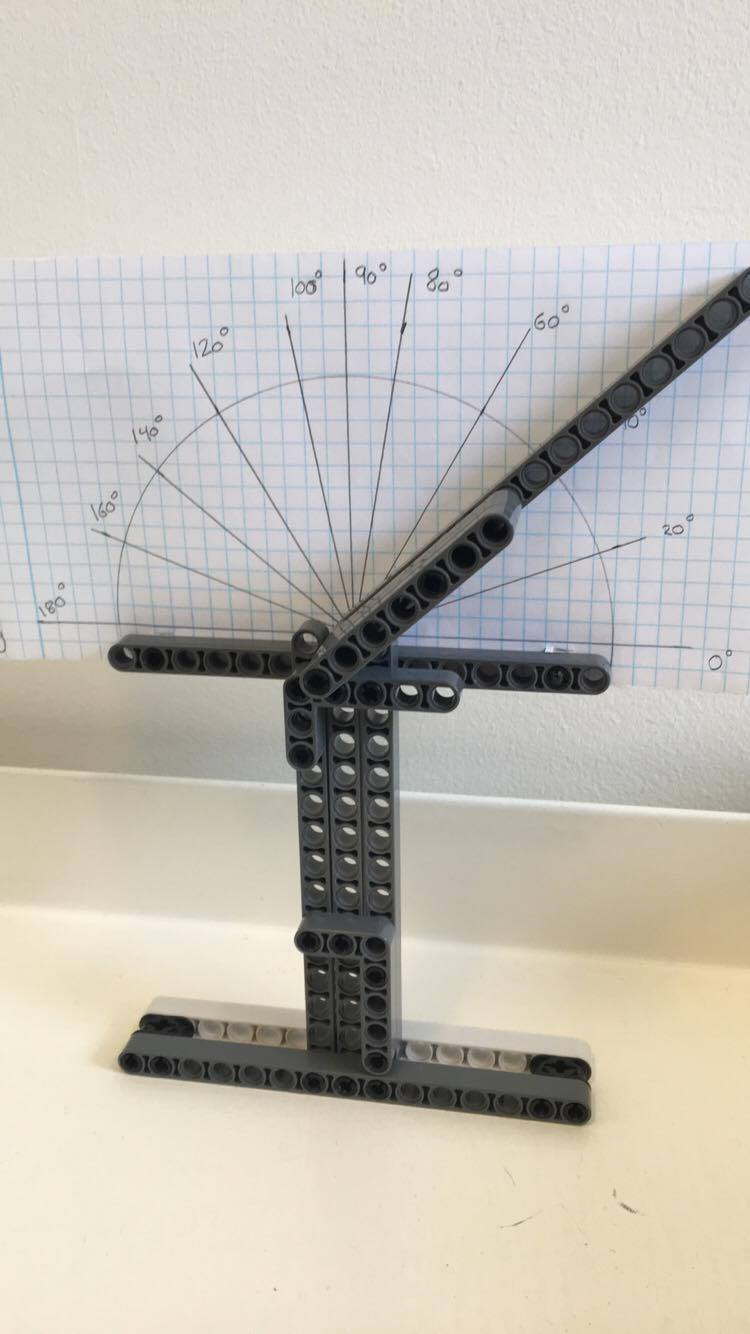
\includegraphics[width=0.3\textwidth]{figures/vinkeltest}
\caption{Vinkeltester, som anvendes under forsøget til at holde accelerometeret i bestemte vinkler}
\label{fig:vinkeltest}
\end{figure}

\subsubsection{Fremgangsmåde for deltest 2}\label{sec:acc_fremgangsmaade}
Der foretages målinger i seks forskellige positioner. Hver position måles tre gange og samles i 10 sekunder ved $100~Hz$. De forskellige positioner er illustreret på \autoref{fig:acc_paavirkning}, og er som følger: 
\begin{itemize}
\item Accelerometeret stilles, så det er lodret opad
\item Accelerometeret stilles, så det er lodret nedad
\item Accelerometeret stilles, så det er vandret mod højre
\item Accelerometeret stilles, så det er vandret mod venstre
\item Accelerometeret ligges plan på bordet opad
\item Accelerometeret ligges plan på bordet nedad
\end{itemize}

\begin{figure}[H]
\centering
\includegraphics[width=0.5\textwidth]{figures/acc_paavirkning}
\caption{Påvirkning af accelerometeret i forskellige positioner. Til venstre måles accelerometeret i lodret plan, til højre øverst vandret og til højre nederst i plan \citep{analogdevices2010}}
\label{fig:acc_paavirkning}
\end{figure}

\subsection{Resultater} 

\subsubsection{Resultater for deltest 2}

De viste resultater heri er for det ene accelerometer\fxnote{resultaterne er fra det røde accelerometer}, da sensitiviten og offsettet ændrer sig hver gang, der udføres et forsøg. Det vil derfor ikke være muligt at fastsætte konstante værdier for sensitivitet og offset, hvorfor det centrale at udlede er metoden til at beregne værdierne, da udregningerne skal foretages ved hvert forsøg.

Ud fra de tre målinger foretaget i de seks forskellige positioner beregnes den gennemsnitlige værdi af målingerne på de forskellige akser, herefter plottes disse i en graf. På denne måde bliver det muligt at se, hvilken akse der påvirkes mest under øvelsen. Målingerne fremgår af \autoref{fig:acc_paavirkning}. 

\begin{figure}[H]
\centering
\includegraphics[width=0.8\textwidth]{figures/paavirkning}
\caption{Påvirkningen af accelerometrets tre akser ved de seks forskellige positioner}
\label{fig:acc_paavirkning}
\end{figure}

Offset beregnes ud fra de målinger, hvor accelerometeret påvirkes med 0 g. Den akse hvor accelerometeret påvirkes med 0 g i de seks positioner fremgår af \autoref{fig:acc_paavirkning}. Resultaterne fra målingerne fremgår af \autoref{Tab:acc_offset}. 

\begin{table}[H]
	\centering
	\begin{tabular}{|l|l|l|}
	\textbf{Målt retning} & \textbf{Målt akse} & \textbf{Offset} \\ \hline
    \textbf{Lodret op} 		& X 		& $1,6793~V$ 	\\ \hline
    \textbf{Lodret op} 		& Z 		& $1,6857~V$ 	 \\ \hline
    \textbf{Lodret ned}		& X 		& $1,6750~V$ 	\\ \hline
    \textbf{Lodret ned}		& Z 		& $1,6806~V$  	\\ \hline
    \textbf{Vandret højre} 	& Y 		& $1,6760~V$    \\ \hline     
    \textbf{Vandret højre} 	& Z 		& $1,6828~V$ 	\\ \hline
    \textbf{Vandret venstre}	& Y 		& $1,6755~V$ 	\\ \hline
    \textbf{Vandret venstre}	& Z 		& $1,6836~V$		\\ \hline
    \textbf{Plan op} 		& X 		& $1,6773~V$		\\ \hline		
    \textbf{Plan op} 		& Y 		& $1,6734~V$    \\ \hline
    \textbf{Plan ned} 		& X 		& $1,6787~V$		\\ \hline
    \textbf{Plan ned} 		& Y 		& $1,6755~V$		\\ \hline
	\end{tabular}\label{Tab:acc_offset}
	\caption{Offsettet beregnet for de forskellige akser, hvor accelerometeret udsættes for en 0 g-påvirkning}
\end{table}

Sensitiviten beregnes ud fra forskellen mellem 0 og 1 g-påvirkningen af accelerometeret. Der hvor accelerometeret er påvirket med 1 g er illustreret på \autoref{fig:acc_paavirkning}. Målingerne fremgår af \autoref{Tab:acc_sensitivitet}. 

\begin{table}[H]
	\centering
	\begin{tabular}{|l|l|l|}
	\textbf{Målt retning} & \textbf{Målt akse} & \textbf{Sensitivitet} \\ \hline
    \textbf{Lodret op} 		& Y		& $0,1092~V/g$ 	\\ \hline
    \textbf{Lodret ned}		& Y 		& $-0,1164~V/g$ 	\\ \hline
    \textbf{Vandret højre} 	& X 		& $0,1130~V/g$     \\ \hline     
    \textbf{Vandret venstre}	& X 		& $-0,1167~V/g$ 	\\ \hline
    \textbf{Plan op} 		& Z 		& $0,1232~V/gV$    	\\ \hline		
    \textbf{Plan ned} 		& Z 		& $-0,1079~V/g$		\\ \hline
	\end{tabular}
	\label{Tab:acc_sensitivitet}
	\caption{Sensitiviteten beregnet for de forskellige akser hvor accelerometeret udsættes for en 1 g-påvirkning}
\end{table}

Ud fra senstitivten beregnes spændingen ved $1^{\circ}$ og $90^{\circ}$ i negativ og positiv retning\fxnote{Er der nødvendig med 1 grad?}. Spændingen svarende til $0^{\circ}$ svarer til den målte offsetværdi som fremgår af \autoref{Tab:acc_offset}. Beregningerne af spændingen ved de valgte grader fremgår af \autoref{Tab:acc_grader} og er beregnet ud fra ligning \autoref{equ:vinkler}.

 \begin{table}[H]
	\centering
	\begin{tabular}{|l|l|l|l|}
	\textbf{Målt retning} & \textbf{Målt akse} & \textbf{Spændingen ved grad} & \textbf{Spændingen ved 90 grader} \\ \hline
    \textbf{Positiv} 	& Y		& $1,7985~V$   	&	$12,7589~V$\\ \hline
    \textbf{Negativ}		& Y		& $1,5692~V$  	&	$-8,0339~V$\\ \hline
    \textbf{Positiv} 	& X 		& $1,7917~V$   	& 	$11,5105~V$ \\ \hline     
    \textbf{Negativ}		& X 		& $1,5614~V$		&	$-8,7982~V$\\ \hline
    \textbf{Positiv} 	& Z 		& $1,7924~V$   	& 	$11,8494~V$	\\ \hline		
    \textbf{Negativ} 	& Z 		& $1,5629~V$		&	$-8,8190~V$ \\ \hline
	\end{tabular}
	\caption{Beregnet spænding ved henholdsvis 1 og 90 grader i positiv og negativ retning}
	\label{Tab:acc_grader}
\end{table}






\chapter{ADC} \label{sec:ADC_bilag}
\section{Opsætning}
I dette afsnit beskrives hvordan ADC'en er opsat. Der fokuseres på de parametre, der er ændret og tilpasset i forhold til dette projekt.

\begin{figure}[H]
	\centering
	\includegraphics[width=0.5\textwidth]{figures/ADC_instillinger_edit.png}
	\caption{ADC's generelle indstillinger, hvor de fremhævede områder viser parametre, der er relevante for dette projekt. Øverste blok til venstre viser instillingsmuligheder for samplings- og clockfrekvens, samt de reelle frekvenser. Nederste blok til venstre viser instillinger for ADC'ens arbejdsområde i forhold til single ended og differential måling. Blokken til højere viser antallet af samples fortaget til at give en gennemsnitlig sample.}
	\label{fig:ADC_GeneralTab}
\end{figure}

\subsection{Bestemmelse af samplingsfrekvens}
Det markerede område øverst til venstre på \autoref{fig:ADC_GeneralTab}, viser indstillingerne for ADC'ens samplingsfrekvens, samt clock frekvens. Ved indstilling af disse frekvenser udregnes en reel samplings- og clockfrekvens. De reelle frekvenser kan variere grundet andre parametre som antal af kanaler, konverteringstid, mm. Yderligere parametre kan findes i databladet for ADC'en. 

I dette projekt opnåes en samplingsfrekvens på $100~Hz$ ved at definere en clockfrekvens på $1600~kHz$ samt ved at justere konverteringstiden af kanalerne, der ses på \autoref{fig:ADC_KanalTab}. Hertil er der pålagt en forsinkelse, således en konverteringstid på $3,32~ms$ per kanal opnås. Dette giver en konverteringstid på $9,96~ms$ for de 3 kanaler, hvilket konfigurationen af ADC'en oplyser som en samplingsfrekvens på $100~Hz$. 

\begin{figure}[H]
	\centering 
	\includegraphics[width=0.5\textwidth]{figures/ADC_instillinger2_edit.png}
	\caption{Indstillinger for de enkelte inputs til ADC'en. Øverste blok viser indstillingsmuligheder for 4 ADC-clocks, der definerer konverteringstiden for kanalerne. Miderste blok viser antallet af kanaler, der defineres. Nederste blok viser indstillingsmuligheder og konvertieringstid for de enkelte kanaler.}
	\label{fig:ADC_KanalTab}
\end{figure}

\subsection{Arbejdsområde for ADC}
Det markerede område nederst til venstre på \autoref{fig:ADC_GeneralTab}, viser indstillingerne for ADC'ens arbejdsområde. Vref definerer størrelsen af arbejdsområdet, hvortil en ekstern reference er valgt. Denne reference sættes til at være identisk med mikrokontrollerens forsyning til acceleromterne på $3,3~V$. Det negative input for single ended målinger sættes til Vss (jord). Dette giver et arbejdsområde for single ended målinger på $0,0~V - 3,3~V$. Da det negative input tilsluttes jord, falder opløsningen $1~bit$, da der ikke kan forekomme negative udslag i arbejdsområdet. 

\subsection{Gennemsnits samples}
Det markerede område til højre på \autoref{fig:ADC_GeneralTab} er indstillingen for, hvor mange samples der anvendes for hver af kanalerne til at repræsentere én konverteret sample. Der benyttes derfor 32 samples til at udregne én gennemsnits-sample, som er den sample, der benyttes i systemet. Dette gøres gældende for kanaler, hvor 'AVG' er afkrydset, som det ses af nederste blok i \autoref{fig:ADC_KanalTab}. Dette er implementeret, da samplingsfrekvensen på $100~Hz$ opretholdes, samt at flere samples, der tilsammen udgør én gennemsnitlig sample, repræsenterer den samplede værdi bedre end én enkelt sample. 






\chapter{Brugersikkerhed} \label{sec:brugersikkerhed}
Når kroppen forbindes med et elektronisk system, opstår der en risiko for at påføre kroppen uønskede fysiologiske reaktioner ved at lade strøm passere gennem kroppen \citep{webster1998}. Disse fysiologiske reaktioner kan ses på \autoref{fig:makromikro}. 

\begin{figure}[H]
\centering
\includegraphics[width=1\textwidth]{figures/makromikro}
\caption{Når $60~Hz$ strøm går gennem hænderne i $1-3~s$, påvirkes en $70~kg$s person forskelligt alt efter, hvor stor en strømstyrke, personen udsættes for \citep{webster1998}.}
\label{fig:makromikro}
\end{figure}

\noindent
Kropsvægt og indgangssted for strømmen afgør, hvilken effekt strømmen har på brugeren. Alt efter, hvordan strømmen løber gennem kroppen og hjertet, kan der opstå mikro- eller makrochok. Hvis hjertet tilføres strøm direkte, og denne derefter går direkte til jord, er det mikrochok. Mikrochok kan ske, hvis en invasiv komponent placeres i direkte kontakt med hjertet. Hvis en person er tilkoblet strøm flere steder, kan der opstå makrochok, da en lille del af strømmen kan gå gennem hjertet. For at undgå makrochok, kan systemet benytte små spændinger og strømstyrke samt batterier for at frakoble personen elnettet \citep{webster1998}.

\section{Sikkerhedsforanstaltninger}
For at undgå mikro- og makrochok kan jording og isolation benyttes som sikkerhedsforanstaltninger. På denne måde kan brugerens sikkerhed opretholdes under brug af systemet. Jording og isolation kombineres ofte, da dette er den mest effektive metode til at sikre brugeren \citep{webster1998}.

\subsection{Jording}
Jording sikrer systemets bruger ved at benytte én fælles referenceværdi for alle systemets blokke. Jording beskytter på denne måde imod mikro- og makrochok, da strømmen vil blive ledt mod jord, ved fejl i kredsløbet. Strømmen afledes dermed fra systemets bruger \citep{webster1998}.

\subsection{Isolation}
Isolation sikrer systemets bruger ved at sørge for, at strøm i form af fejl- eller lækstrømme ikke løber fra én del af systemet til en anden, da dette kan medføre makrochok. Ved at isolere, er det dermed ikke muligt for fejl- eller lækstrømme at nå systemets bruger \citep{webster1998}. 

\section{Implementering af brugersikkerhed}
I dette system kombineres jording og isolation for at sikre systemets bruger mest effektivt. Systemet jordes ved at have en fælles jord for alle systemets komponenter - denne kommer fra spændingsforsyningens GND-terminaler, der er illustreret på \autoref{fig:spaendingsforsyning}. Isolation sikres ved at lade systemet være adskilt fra computeren, der benyttes til datavisualisering, ved brug af den trådløse BLE-forbindelse. Derudover adskilles systemet fra elnettet ved brug af batterier som spændingsforsyning. På denne måde kommer brugeren af systemet ikke i forbindelse med høje spændinger eller strømme. 



%\fi
\end{document}
